%% Copyright 2007-2020 Elsevier Ltd
%DIF LATEXDIFF DIFFERENCE FILE
%DIF DEL OrigSubmissionLatticeBoltz_SOP.tex   Fri Sep 30 21:49:30 2022
%DIF ADD LatticeBoltz_SOP.tex                 Fri Oct  7 15:54:03 2022
%% 
%% This file is part of the 'Elsarticle Bundle'.
%% ---------------------------------------------
%% 
%% It may be distributed under the conditions of the LaTeX Project Public
%% License, either version 1.2 of this license or (at your option) any
%% later version.  The latest version of this license is in
%%    http://www.latex-project.org/lppl.txt
%% and version 1.2 or later is part of all distributions of LaTeX
%% version 1999/12/01 or later.
%% 
%% The list of all files belonging to the 'Elsarticle Bundle' is
%% given in the file `manifest.txt'.
%% 
%% Template article for Elsevier's document class `elsarticle'
%% with Harvard style bibliographic references

%\documentclass[preprint,12pt,authoryear]{elsarticle}
%\documentclass[3p, 12pt,authoryear]{elsarticle}
\documentclass[final, 3p, times, authoryear]{elsarticle}

%% Use the option review to obtain double line spacing
%% \documentclass[authoryear,preprint,review,12pt]{elsarticle}

%% Use the options 1p,twocolumn; 3p; 3p,twocolumn; 5p; or 5p,twocolumn
%% for a journal layout:
%% \documentclass[final,1p,times,authoryear]{elsarticle}
%% \documentclass[final,1p,times,twocolumn,authoryear]{elsarticle}
%% \documentclass[final,3p,times,authoryear]{elsarticle}
%% \documentclass[final,3p,times,twocolumn,authoryear]{elsarticle}
%% \documentclass[final,5p,times,authoryear]{elsarticle}
%% \documentclass[final,5p,times,twocolumn,authoryear]{elsarticle}

%% For including figures, graphicx.sty has been loaded in
%% elsarticle.cls. If you prefer to use the old commands
%% please give \usepackage{epsfig}

%% The amssymb package provides various useful mathematical symbols
\usepackage{amssymb}
%% The amsthm package provides extended theorem environments
\usepackage{amsmath,amsthm}

%% The lineno packages adds line numbers. Start line numbering with
%% \begin{linenumbers}, end it with \end{linenumbers}. Or switch it on
%% for the whole article with \linenumbers.
%% \usepackage{lineno}

\usepackage{hyperref}
\usepackage{xcolor}
\hypersetup{
    colorlinks,
    linkcolor={red!50!black},
    citecolor={blue!50!black},
    urlcolor={blue!80!black}
}

\usepackage{multirow}
\usepackage{pgfplots}
\usepackage{arydshln}
\usepackage{paralist}
\usepackage{multicol}
\usepackage{booktabs}
\usepackage{pbox}
%DIF 65a65
\usepackage{makecell} %DIF > 
%DIF -------

%% Comments
\newif\ifcomments\commentstrue

\ifcomments
\newcommand{\authornote}[3]{\textcolor{#1}{[#3 ---#2]}}
\newcommand{\todo}[1]{\textcolor{red}{[TODO: #1]}}
\else
\newcommand{\authornote}[3]{}
\newcommand{\todo}[1]{}
\fi

\newcommand{\wss}[1]{\authornote{blue}{SS}{#1}} %Spencer Smith
\newcommand{\jc}[1]{\authornote{red}{JC}{#1}} %Jacques Carette
\newcommand{\zm}[1]{\authornote{magenta}{MN}{#1}} %Zahra Keshavarz-Motamed
\newcommand{\pmm}[1]{\authornote{cyan}{PM}{#1}} %Peter Michalski

\newcommand{\notdone}[1]{\textcolor{red}{#1}}
\newcommand{\done}[1]{\textcolor{black}{#1}}

% For easy change of table widths
\newcommand{\colZwidth}{1.0\textwidth}
\newcommand{\colAwidth}{0.24\textwidth}
\newcommand{\colBwidth}{0.76\textwidth}
\newcommand{\colCwidth}{0.28\textwidth}
\newcommand{\colDwidth}{0.72\textwidth}
\newcommand{\colEwidth}{0.33\textwidth}
\newcommand{\colFwidth}{0.67\textwidth}
\newcommand{\colGwidth}{0.5\textwidth}
\newcommand{\colHwidth}{0.28\textwidth}

\newcounter{comnum} %Commonality Number
\newcommand{\cthecomnum}{C\thecomnum}
\newcommand{\cref}[1]{C\ref{#1}}

\newcounter{varnum} %Variability Number
\newcommand{\vthevarnum}{V\thevarnum}
\newcommand{\vref}[1]{V\ref{#1}}

\newcounter{parnum} %Parameter of Variation Number
\newcommand{\ptheparnum}{P\theparnum}
\newcommand{\pref}[1]{P\ref{#1}}

\newcommand{\CC}{C\nolinebreak\hspace{-.05em}\raisebox{.4ex}{\small\bf
+}\nolinebreak\hspace{-.10em}\raisebox{.4ex}{\small\bf +}}

\newcommand{\esp}{ESPResSo\nolinebreak\hspace{-.05em}\raisebox{.4ex}{\small\bf
+}\nolinebreak\hspace{-.10em}\raisebox{.4ex}{\small\bf +}}

\newcounter{rqnum} %research question number
\newcommand{\rqtherqnum}{RQ`'\therqnum}
\newcommand{\rqref}[1]{RQ\ref{#1}}

\newcounter{pnum} %pain point number
\newcommand{\ppthepnum}{P`'\thepnum}
\newcommand{\ppref}[1]{P\ref{#1}}

\newcounter{bpnum} %best practice number
\newcommand{\bpthepnum}{BP`'\thebpnum}
\newcommand{\bpref}[1]{BP\ref{#1}}

\journal{Archives of Computational Methods in Engineering}
%DIF PREAMBLE EXTENSION ADDED BY LATEXDIFF
%DIF UNDERLINE PREAMBLE %DIF PREAMBLE
\RequirePackage[normalem]{ulem} %DIF PREAMBLE
\RequirePackage{color}\definecolor{RED}{rgb}{1,0,0}\definecolor{BLUE}{rgb}{0,0,1} %DIF PREAMBLE
\providecommand{\DIFaddtex}[1]{{\protect\color{blue}\uwave{#1}}} %DIF PREAMBLE
\providecommand{\DIFdeltex}[1]{{\protect\color{red}\sout{#1}}}                      %DIF PREAMBLE
%DIF SAFE PREAMBLE %DIF PREAMBLE
\providecommand{\DIFaddbegin}{} %DIF PREAMBLE
\providecommand{\DIFaddend}{} %DIF PREAMBLE
\providecommand{\DIFdelbegin}{} %DIF PREAMBLE
\providecommand{\DIFdelend}{} %DIF PREAMBLE
\providecommand{\DIFmodbegin}{} %DIF PREAMBLE
\providecommand{\DIFmodend}{} %DIF PREAMBLE
%DIF FLOATSAFE PREAMBLE %DIF PREAMBLE
\providecommand{\DIFaddFL}[1]{\DIFadd{#1}} %DIF PREAMBLE
\providecommand{\DIFdelFL}[1]{\DIFdel{#1}} %DIF PREAMBLE
\providecommand{\DIFaddbeginFL}{} %DIF PREAMBLE
\providecommand{\DIFaddendFL}{} %DIF PREAMBLE
\providecommand{\DIFdelbeginFL}{} %DIF PREAMBLE
\providecommand{\DIFdelendFL}{} %DIF PREAMBLE
%DIF HYPERREF PREAMBLE %DIF PREAMBLE
\providecommand{\DIFadd}[1]{\texorpdfstring{\DIFaddtex{#1}}{#1}} %DIF PREAMBLE
\providecommand{\DIFdel}[1]{\texorpdfstring{\DIFdeltex{#1}}{}} %DIF PREAMBLE
%DIF LISTINGS PREAMBLE %DIF PREAMBLE
\RequirePackage{listings} %DIF PREAMBLE
\RequirePackage{color} %DIF PREAMBLE
\lstdefinelanguage{DIFcode}{ %DIF PREAMBLE
%DIF DIFCODE_UNDERLINE %DIF PREAMBLE
  moredelim=[il][\color{red}\sout]{\%DIF\ <\ }, %DIF PREAMBLE
  moredelim=[il][\color{blue}\uwave]{\%DIF\ >\ } %DIF PREAMBLE
} %DIF PREAMBLE
\lstdefinestyle{DIFverbatimstyle}{ %DIF PREAMBLE
	language=DIFcode, %DIF PREAMBLE
	basicstyle=\ttfamily, %DIF PREAMBLE
	columns=fullflexible, %DIF PREAMBLE
	keepspaces=true %DIF PREAMBLE
} %DIF PREAMBLE
\lstnewenvironment{DIFverbatim}{\lstset{style=DIFverbatimstyle}}{} %DIF PREAMBLE
\lstnewenvironment{DIFverbatim*}{\lstset{style=DIFverbatimstyle,showspaces=true}}{} %DIF PREAMBLE
%DIF END PREAMBLE EXTENSION ADDED BY LATEXDIFF

\begin{document}

\begin{frontmatter}

%% Title, authors and addresses

%% use the tnoteref command within \title for footnotes;
%% use the tnotetext command for theassociated footnote;
%% use the fnref command within \author or \affiliation for footnotes;
%% use the fntext command for theassociated footnote;
%% use the corref command within \author for corresponding author footnotes;
%% use the cortext command for theassociated footnote;
%% use the ead command for the email address,
%% and the form \ead[url] for the home page:
%% \title{Title\tnoteref{label1}}
%% \tnotetext[label1]{}
%% \author{Name\corref{cor1}\fnref{label2}}
%% \ead{email address}
%% \ead[url]{home page}
%% \fntext[label2]{}
%% \cortext[cor1]{}
%% \affiliation{organization={},
%%            addressline={}, 
%%            city={},
%%            postcode={}, 
%%            state={},
%%            country={}}
%% \fntext[label3]{}

\title{State of the Practice for Lattice Boltzmann Method Software}

%% use optional labels to link authors explicitly to addresses:
%% \author[label1,label2]{}
%% \affiliation[label1]{organization={},
%%             addressline={},
%%             city={},
%%             postcode={},
%%             state={},
%%             country={}}
%%
%% \affiliation[label2]{organization={},
%%             addressline={},
%%             city={},
%%             postcode={},
%%             state={},
%%             country={}}

%\author{Anonymous}
\author[CAS]{Spencer Smith}
\author[CAS]{Peter Michalski}
\author[CAS]{Jacques Carette}
\author[ME]{Zahra Keshavarz-Motamed}

\affiliation[CAS]{organization={McMaster University, Computing and Software
Department}, %Department and Organization
            addressline={1280 Main Street West}, 
            city={Hamilton},
            postcode={L8S 4K1}, 
            state={Ontario},
            country={Canada}}

\affiliation[ME]{organization={McMaster University, Mechanical Engineering}, %Department and Organization
            addressline={1280 Main Street West}, 
            city={Hamilton},
            postcode={L8S 4K1}, 
            state={Ontario},
            country={Canada}}

\begin{abstract}

    We analyze the state of software development practice for Lattice Boltzmann
    solvers by quantitatively and qualitatively measuring and comparing 24
    software packages for 10 software qualities (installability, correctness/
    verifiability, reliability, robustness, usability, maintainability,
    reusability, understandability, visibility/transparency and
    reproducibility). Our reproducible analysis method employs a measurement
    template (containing 108 measures that are manually and automatically
    extracted from the project repository) and developer interviews (consisting
    of 20 questions). After measuring, we rank the software using the Analytic
    Hierarchy Process (AHP). Our ranking is roughly consistent with GitHub stars
    ranking, suggesting at least a partial correlation between the use of best
    practices and popularity. We find the state of the practice to be healthy,
    with 67\% of the measured packages ranking in the top \DIFdelbegin \DIFdel{five }\DIFdelend \DIFaddbegin \DIFadd{two }\DIFaddend for at least \DIFdelbegin \DIFdel{one
    quality}\DIFdelend \DIFaddbegin \DIFadd{two
    qualities}\DIFaddend , the majority of LBM generated artifacts corresponding to general
    recommendations from research software developers, common use of version
    control (67\% of packages) and the adoption of a quasi-agile development
    process.  Areas of best practice to potentially improve include adoption of
    continuous integration, API documentation and enforcement of programming
    style guides.  We interviewed four developers to gain insight into their
    current pain points. Identified challenges include lack of development time,
    lack of funding, and difficulty with ensuring correctness.  Developers are
    addressing these pain points by designing for change, circumventing the
    oracle problem and prioritizing documentation and usability. For future
    improvements we suggest the following: employing linters, conducting
    rigorous peer reviews, writing and submitting more papers on software,
    growing the number of contributors by following current recommendations for
    open source projects, and augmenting the theory manuals to include more
    requirements specification relevant information.

\end{abstract}

%%Graphical abstract
%\begin{graphicalabstract}
%\includegraphics{grabs}
%\end{graphicalabstract}

%%Research highlights
%\begin{highlights}
%\item Research highlight 1
%\item Research highlight 2
%\end{highlights}

\begin{keyword}
	Lattice Boltzmann Method (LBM), research software, software engineering,
	software quality, Analytic Hierarchy Process (AHP)
\end{keyword}

\end{frontmatter}

%% \linenumbers

\section{Introduction} \label{secIntro}

We analyze the development of Computational Fluid Dynamics (CFD) software
packages that use the Lattice Boltzmann Method (LBM). LBM packages form a family
of algorithms for simulating single-phase and multiphase fluid flows, often
incorporating additional physical complexities \citep{chen1998lattice}, such as
reflective and non-reflective boundaries. LBM solvers consider the behaviour of a
collection of particles as a single unit at the mesoscopic scale, which lies
between the nanoscopic and microscopic scales. These solvers predict the
positional probability of a collection of particles moving through a lattice
structure following a two-step process: i) streaming, where the particles move
along the lattice via links; and, ii) colliding, where particles transfer energy
and momentum when they collide \citep{bao2011lattice}. As an example of an
important application of LBM, Figure~\ref{Fig_coarctation} shows the flow in a
defective aorta pre- and post-medical intervention. LBM has several advantages
over conventional CFD methods, including a simple calculation procedure,
improved parallelization, and robust handling of complex geometries
\citep{ganji2015application}.

\begin{figure}[h!]
	\begin{center}
		\includegraphics[width=0.7\textwidth]{./figures/FlowModellingCoarctation.pdf}
		\caption{LBM (and Lattice Poisson-Boltzmann) computed flow (velocity
		magnitude, turbulent kinetic energy and time averaged wall shear stress)
		in an aorta with a coarctation (narrowing of the artery) and a major
		aneurysm (a ballooning of the artery wall) downstream of the
		coarctation, pre and post intravascular stent intervention
		\citep{SadeghiEtAl2020}}.
		\label{Fig_coarctation}
	\end{center}
\end{figure}

A small sample of safety and mission-critical applications of LBM includes the
following: designing fuel cells \citep{ZhangEtAl2018}, modelling groundwater
flow \citep{AnwarAndSukop2009}, and analyzing the flow of blood in the
cardiovascular system \citep{SadeghiEtAl2022b, SadeghiEtAl2022,
SadeghiEtAl2020}.  As these examples illustrate, engineers and scientists use
LBM for tackling problems that impact such areas as environmental policy,
manufacturing, and health and safety. Given the critical applications of LBM,
users worry about software qualities like reliability, robustness,
reproducibility, performance, correctness, and verifiability.  Since their time
is valuable, developers of LBM libraries have additional quality concerns,
including maintainability, reusability, and understandability.  With these
quality considerations in mind, and the potentially overwhelming number of
choices for existing LBM libraries, the time is right to assess the state of the
practice. Therefore, we analyze the current state of LBM software development
and compare it to the development practices employed for research software in
general.  We want to highlight success stories that LBM developers can share
amongst their community, and with the broader research software community, while
at the same time looking for areas for potential future improvement.

We use 10 research questions to structure and focus our discussion. These
questions drive our methodology \citep{SmithEtAl2021, SmithAndMichalski2022}.
For each question below, we point to the section that contains our answer.  We
start with identifying the examples of LBM software where we have access to the
source code:

\begin{enumerate}
	\item[RQ\refstepcounter{rqnum}\therqnum \label{RQ_WhatProjects}:] What LBM
	software projects exist, with the constraint that the source code must be
	available for all identified projects? (Section~\ref{methodology})
\end{enumerate}

We next wish to assess the representative software to determine how well they
apply current software development best practices.  By \emph{best practices}, we
mean methods, techniques, and tools that are generally believed to improve
software development, like testing and documentation.  We categorize our best
practices around software qualities (Section~\ref{softwarequalities}).  At this
point in the process, to remove potential user/developer bias, we base our
assessment only on publicly available artifacts, where artifacts are the
documents, scripts, and code that we find in a project's public repository.
Example artifacts include requirements, specifications, user manuals, unit test
cases, system tests, usability tests, build scripts, API (Application
Programming Interface) documentation, READMEs, license documents, process
documents, and code. Following best practices does not guarantee popularity, so
we also compare our ranking to how the user community ranks the identified
projects.

\begin{enumerate}
	\item [RQ\refstepcounter{rqnum}\therqnum \label{RQ_HighestQuality}:] Which
	of the projects identified in \rqref{RQ_WhatProjects} follow current best
	practices, based on evidence found by experimenting with the software and
	searching the artifacts available in each project's repository?
	(Section~\ref{AHPresults})
	\item [RQ\refstepcounter{rqnum}\therqnum \label{RQ_CompareHQ2Popular}:] How
	similar is the list of top projects identified in \rqref{RQ_HighestQuality}
	to the most popular projects, as viewed by the scientific community?
	(Section~\ref{repmetrics})
\end{enumerate}

To understand the state of the practice, we wish to learn the frequency with
which different artifacts appear, the types of development tools used, and the
methodologies used for software development.  With this data, we can ask
questions about how LBM software compares to other research software.  For cases
where data is available, we can compare to other specific domains of research
software, like medical imaging \citep{Dong2021} and ocean modelling
\citep{JungEtAl2022}.  However, most of the literature on the state of the
practice does not focus on specific domains, but rather on all research software
\citep{SmithAndMichalski2022}. We will refer to studies and guidelines that do
not distinguish an application domain as \emph{research software in general}. By
comparing LBM software to research software in general we can determine how LBM
follows the trends from other developer communities and how it is different.

\begin{enumerate}
    \item [RQ\refstepcounter{rqnum}\therqnum \label{RQ_CompareArtifacts}:] How
	do LBM projects compare to research software in general with respect to the
	artifacts present in their repositories?
	(Section~\ref{Sec_CompareArtifacts})
	\item [RQ\refstepcounter{rqnum}\therqnum \label{RQ_CompareToolsProjMngmnt}:]
	How do LBM projects compare to research software in general with respect to
	the use of tools (Section~\ref{Sec_CompareTools}) for:
	\begin{enumerate} 
		\item [\rqref{RQ_CompareToolsProjMngmnt}.a] development; and,
		\item [\rqref{RQ_CompareToolsProjMngmnt}.b] project management?
	\end{enumerate}
	\item [RQ\refstepcounter{rqnum}\therqnum \label{RQ_CompareMethodologies}:]
	How do LBM projects compare to research software in general with respect to
	principles, processes, and methodologies used?
	(Section~\ref{Sec_CompareMethodologies})
\end{enumerate}	

Only so much information can be gleaned by looking at software repositories.  To
gain additional insight, we need to interview developers.  We need to learn
their concerns and how they deal with them; we need to understand their pain
points. We wish to know what practices top LBM projects use, so that
others can potentially emulate these practices. Part of our goal is to identify new
practices that LBM developers can adopt to improve their software in the future.
The question below cover these points: 

\begin{enumerate}
	\item [RQ\refstepcounter{rqnum}\therqnum \label{RQ_PainPoints}:] What are
	the pain points for developers working on LBM software projects?
	(Section~\ref{painpoints})
	\item [RQ\refstepcounter{rqnum}\therqnum \label{RQ_ComparePainPoints}:] How
	do the pain points of developers from LBM compare to the pain points
	for research software in general? (Section~\ref{painpoints})
	\item [RQ\refstepcounter{rqnum}\therqnum \label{RQ_Concerns}:] For LBM
	developers what specific best practices address their pain points
	and software quality concerns? (Section~\ref{Sec_AddressConcerns})
	\item [RQ\refstepcounter{rqnum}\therqnum \label{RQ_Recommend}:]
	What research software development practices could potentially address the
	pain point concerns identified in \rqref{RQ_PainPoints}.
	(Section~\ref{Sec_Recommendations})
\end{enumerate}

We investigate the research questions by applying the general methodology
summarized in \citet{SmithEtAl2021, SmithAndMichalski2022}. The specific
application of the methodology to LBM is reviewed in Section~\ref{methodology},
with the full details in \DIFdelbegin \DIFdel{Anonymous (xxxx)}
\DIFdelend \citet{Michalski2021}. Our methodology updates
an approach used in prior assessments of domains like Geographic Information
Systems \citep{SmithEtAl2018_arXivGIS}, Mesh Generators \citep{SmithEtAl2016},
Oceanographic Software \citep{smith2015state}, Seismology software
\citep{SmithEtAl2018}, statistical software for psychology
\citep{SmithEtAl2018_StatSoft} and medical image analysis software
\citep{Dong2021}.

We start by identifying 24 LBM software packages.  We then approximately measure
the application of best practices for each package by filling in a grading
template. Our analysis points to areas where some LBM software packages fall
short of current best practices.  Our intention is not to criticize any existing
packages, especially since not every project is actively maintained.  Moreover,
we recognize that not every project needs to achieve the highest possible
quality.  However, rather than delve into the nuances of which software can
justify compromising which practice we conducted our comparison under the ideal
assumption that every project can have sufficient resources to match best
practices.

Compared with our previous methodology (as used in \citet{SmithEtAl2016} for
instance) %(Anonymous, xxxx)\footnotemark[1] %DOUBLE BLIND
measuring the application of best practices now also includes repository based
metrics, such as the number of files, number of lines of code, percentage of
issues that are closed, etc.  We rank the software with the Analytic Hierarchy
Process (AHP), using the quantitative data from the grading template. After
this, as another addition to our previous methodology, we interview some
development teams to understand the status of their development processes. We
next answer the research questions using the collected quantitative and
qualitative data (Sections~\ref{methodology} to~\ref{Sec_Recommendations}).
Finally, we summarize the threats to validity (Section~\ref{threats}) and the
final conclusions and recommendations (Section~\ref{conclusion}).

\section{Methodology} \label{methodology}

We apply our methodology for evaluating the state of the practice of research
software \citep{SmithEtAl2021, SmithAndMichalski2022} % DOUBLE BLIND
to the specific domain of
LBM software.  Since we group best practices around conventional software
qualities, the first section below provides definitions for the qualities of
interest (Section~\ref{softwarequalities}), along with information on how to
measure these qualities. The following section
(Section~\ref{Sec_OverallProcess}) provides an overview of the steps we used to
select, measure and compare LBM software.  The remaining sections
(Sections~\ref{identifysoftware} to~\ref{sec_vet_software_list}) provide details
on each step in the methodology. 

\subsection{Measuring Software Qualities} \label{softwarequalities}

To ensure our assessment of best practices is organized and complete, we centre
our measurements around software qualities. For completeness, we use the list of
software engineering qualities from \citet[p.\ 17--33]{GhezziEtAl2003},
excluding interoperability, productivity, and timeliness. We excluded
interoperability because our focus is on LBM software alone, not its interaction
with other software. Our exclusion of the other two qualities is because they
are process qualities, and our focus is on product qualities. We added
installability to our list since potential users will ignore software they
cannot install.  Since the scientific method depends on reproducibility, we also
added this quality. Below we provide information on each quality, including
details on how they are measured. 

\begin{description}

	\item[Installability] Installability is measured by the effort required for
	the installation, uninstallation, or reinstallation of a software product in
	a specified environment \citep{ISO/IEC25010, lenhard2013measuring}. In our
	case, the effort includes the following: time spent finding and
	understanding the installation instructions, the person-time and resources
	spent performing the installation procedure, and the absence or ease of
	overcoming system compatibility issues. An installability score improves if
	the software has means to validate the installation and instructions for
	uninstallation.

	\item[Correctness] A software program is correct if it behaves according to
	its stated specifications \citep[p.\ 17]{GhezziEtAl2003}. Therefore,
	measuring correctness requires that a specification is available. However,
	research software is unlikely to have an explicit specification. As a
	consequence, correctness often cannot be measured directly. We assess
	correctness indirectly by looking for the following: availability of a
	requirements specification, reference to domain theory, and explicit use of
	tools and/or techniques for building confidence, such as documentation
	generators and software analysis tools.

	\item[Verifiability] An artifact (like code, or a theory manual) is
	verifiable if, and only if, every statement therein is verifiable. A
	statement is verifiable if, and only if, there exists some finite
	cost-effective process with which a person or machine can check that each
	statement is correct (adapted from recommended practice for requirements
	specifications \citep{IEEE1998}). Similar to correctness, verifiability
	increases with the presence of a specification and with references and
	pointers to domain knowledge. A good measure of verifiability results from
	the following: availability of well-written tutorials that include expected
	output, software unit tests, and evidence of Continuous Integration (CI).
	Our process measures correctness and verifiability together.

	\item[Reliability] Reliability is measured by the probability of
	failure-free operation of a computer program in a specified environment for
	a specified time \citep[p.\ 357]{GhezziEtAl2003}, \citep{musa1987software}.
	The absence of errors during installation and use increases the reliability
	score. Recoverability from errors also improves reliability.

	\item[Robustness] Software possesses the characteristic of robustness if it
	behaves ``reasonably'' in two situations: i) when it encounters
	circumstances not anticipated in the requirements specification; and ii)
	when the software inputs violate the requirements specification assumptions
	\citep{boehm2007software}, \citep[p.\ 19]{GhezziEtAl2003}. A good measure of
	robustness correlates with a reasonable reaction to unexpected input,
	including data of the wrong type, empty input, or missing files or links.
	Examples of reasonable reactions include an appropriate error message and the
	ability to recover the system.

	\item[Performance] Performance is measured by the degree to which a system
	or component accomplishes its designated functions within given constraints,
	such as speed (database response times, for instance), throughput
	(transactions per second), capacity (concurrent usage loads), and timing
	(hard real-time demands) \citep{IEEEStdGlossarySET1990, wiegers2003softreq}.
	Our state of the practice assessment does not directly quantitatively
	measure performance. Instead, we check the documentation for each software
	package looking for information alluding to consideration of performance,
	such as testing results or parallelization instructions. 

	\item[Usability] Usability is measured by the extent to which a software
	product can be used by specified users to achieve specified goals with
	effectiveness, efficiency, and satisfaction in a specified context of use
	\citep{nielsonusability}. We assume that high usability correlates with
	the presence of documentation, including tutorials, manuals, defined
	user characteristics, and user support. Preferably the user support model
	will have avenues to contact developers and report issues.

	\item[Maintainability] A measure of maintainability is the effort with which
	a software system or component can be modified to correct faults, improve
	performance or other attributes, and satisfy new requirements
	\citep{IEEEStdGlossarySET1990, boehm2007software}. In the current work, we
	measure maintainability by the quality of the documentation and the presence
	of version control and issue tracking. There are many documentation
	artifacts that can improve maintainability, including user and developer
	manuals, specifications, README files, change logs, release notes,
	publications, forums, and instructional websites. We also ask developers
	if they considered the ease of future changes when developing their
	software. 

	\item[Reusability] Reusability refers to the extent to which components of a
	software package can be used with or without adaptation in other software
	packages \citep{kalagiakos2003non}. A good indicator of reusability is many
	easily reusable components. Therefore, we look for high modularization,
	which we define as the presence of small components with well-defined
	interfaces. For this state of the practice assessment, we assume that a good
	measure of reusability correlates with a high number of code files, and the
	availability of API documentation. 

	\item[Understandability] Understandability is measured by the capability of
	the software package to enable the user to understand its suitability and
	function \citep{ISO9126}. It is an artifact-dependent quality.
	Understandability is different for the user interface, source code, and
	documentation. In this state of the practice analysis, understandability
	focuses on the source code. We measure it by the consistency of formatting
	style, the extent of modularization, the explicit identification of coding
	standards, the presence of meaningful identifiers, and the clarity of
	comments.

	\item[Visibility and Transparency] Visibility and transparency refer to the
	extent to which all the steps of a software development process, and its
	current status, are conveyed clearly \citep[p.\ 32]{GhezziEtAl2003}. In this
	state of the practice assessment a good measure of visibility and
	transparency correlates with a well-defined development process,
	documentation of the development process and environment, and software
	version release notes.

	\item[Reproducibility] Software achieves reproducibility if another
	developer can take the original code and input data, run it, and obtain the
	original output \citep{BenureauAndRougier2017}. We measure reproducibility
	qualitatively by asking developers if they have any concerns that their
	computational results are not reproducible, and if they have taken any
	steps to ensure reproducibility.

\end{description}

\subsection{Overall Process} \label{Sec_OverallProcess}

Our assessment process consists of the following steps: 

\begin{enumerate}
	\item List candidate software packages for the domain.
	(Section~\ref{identifysoftware})
	\item Filter the software package list. (Section~\ref{filtersoftware})
	\item Gather the source code and documentation for each software package.
	\item Collect quantitative measures from the project repositories.
	(Section~\ref{empiricalmeasures})
	\item Measure using the measurement template.  The full measurement template
	can be found in \citet{SmithEtAl2021}. %DOUBLE BLIND
	(Section~\ref{empiricalmeasures})
	\item Rank the software using AHP. (Section~\ref{AHP})
	\item Interview the developers. (Section~\ref{SecSurvey})
	\item Analyze the domain. (Section~\ref{SecDomainAnalysis})
	\item Analyze the results and answer the research questions.
\end{enumerate}

\noindent The above steps depend on interaction with a Domain Expert partner, as
discussed in Section~\ref{sec_vet_software_list}.

\subsection{Identify Candidate Software} \label{identifysoftware}

To answer~\rqref{RQ_WhatProjects} we identify existing LBM projects through
search engine queries targeting authoritative lists. We find the software in
scholarly articles, \href{https://github.com/} {GitHub} and
\href{https://swmath.org/} {swMATH}. The Domain Expert
(Section~\ref{sec_vet_software_list}) also helps with selecting the candidate
software.  We build our list based on the following criteria:

\begin{enumerate}
	\item The software functionality must fall within the identified domain.
	\item The source code must be viewable.
	\item The empirical measures should be available, which implies a preference
	for GitHub-style repositories.
	\item The software cannot be marked as incomplete, or in an initial state of
	development.
\end{enumerate}

\noindent Our initial list had 45 packages, including some that we later found
to be unusable because of incompleteness, or an absence of publicly available
source code.

\subsection{Filter the Software List} \label{filtersoftware}

To reduce the length of the list and to answer~\rqref{RQ_WhatProjects}, we
filter the initial list of 45 packages. We apply the following filters in the
priority order listed. 

\begin{enumerate}
	\item Scope: We remove software by narrowing what functionality we
    consider within the scope of the domain.
	\item Usage: We eliminate software if its installation procedure is
	missing or unclear.
	\item Age: We eliminate the older software packages (with age measured by
	the last date of a change), except when an older software package appears to
	be highly recommended and currently in use. 
\end{enumerate}

For the third item in the above filter, we categorize software packages as
`alive' if documentation updates happened within the last 18 months, and `dead'
otherwise. 

\begin{table}[ht!]
	\begin{center}
		\begin{tabular}{ p{3cm}p{2cm}p{2cm}p{5.5cm} }
			\toprule
			Name & Released & Updated & Relevant Publication\\
			\midrule
			\href{https://www.ccp5.ac.uk/sites/www.ccp5.ac.uk/files/dl_meso/data/dl_meso_2.7.zip}{DL\_MESO (LBE)} & unclear & 2020 Mar&\citep{seaton2013dlmeso}\\
			\href{https://github.com/espressomd/espresso}{ESPResSo} & 2010 Nov & 2020 Jun&\citep{weik2019espresso}\\
			\href{https://github.com/espressopp/espressopp}{ESPResSo++} & 2011 Feb & 2020 Apr&\citep{halverson2013espresso++}\\
			\href{https://github.com/mabau/lbmpy}{lbmpy}& unclear  & 2020 Jun & \citep{bauer2021lbmpy}\\
			\href{https://github.com/Olllom/lettuce}{lettuce} & 2019 May & 2020 Jul&\citep{bedrunka2021lettuce}\\
			\href{https://github.com/ludwig-cf/ludwig}{Ludwig} & 2018 Aug & 2020 Jul&\citep{desplat2001ludwig}\\
			\href{https://github.com/aharwood2/LUMA}{LUMA} & 2016 Nov   & 2020 Feb &\citep{harwood2018luma}\\
			\href{http://hg.savannah.gnu.org/hgweb/mechsys/file/tip/}{MechSys} & 2008 Jun    & 2021 Oct &\citep{galindo2013coupled}\\
			\href{https://osdn.net/projects/apes/scm/hg/musubi/}{Musubi} & 2013 Sep & 2019 Aug &\citep{hasert2014complex}\\
			\href{https://www.openlb.net/download/}{OpenLB} & 2007 Jul & 2019 Oct &\citep{heuveline2010openlb}\\
			\href{https://gitlab.com/unigespc/palabos}{Palabos} & unclear & 2020 Jul &\citep{latt2021palabos}\\
			\href{https://github.com/pylbm/pylbm}{pyLBM} & 2015 Jun&   2020 Jun &\\
			\href{https://github.com/sailfish-team/sailfish}{Sailfish} & 2012 Nov & 2019 Jun & \citep{januszewski2014sailfish}\\
			\href{https://github.com/CFD-GO/TCLB}{TCLB} & 2013 Jun  & 2020 Apr & \citep{rokicki2016adjoint}\\
			\href{https://i10git.cs.fau.de/walberla/walberla}{waLBerla} & 2008 Aug & 2020 Jul & \citep{bauer2021walberla}\\
			\bottomrule
		\end{tabular}
		\caption{Alive Software Packages (Sorted Alphabetically)} \label{alivepackages}
	\end{center}
\end{table}

Filtering by scope, usage, and age decreased the size of the list to 23
packages. We removed 22 packages for the following reasons: we cannot install
them, they are incomplete, source code is not publicly available, we are not
licensed to use them, or the project is out of scope. \citet{Michalski2021}
lists the eliminated software packages. Of the remaining 23 packages, we kept
some despite their `dead` status because of their presence on authoritative LBM
software lists and because of their surface excellence. After the initial
measurement exercise, which took place in mid-2020, we added one more package in
January 2022: Musubi. We found Musubi after our initial search, but we felt
obliged to include it since it clearly fits our criteria. Time constraints meant
we could not update the previous manual data collection, but we did redo the
automated data collection.

The final list of 24 software packages is in two tables.
Table~\ref{alivepackages} lists packages that fall into the `alive' category as
of mid-2020 (January 2022 for Musubi), and Table~\ref{deadpackages} lists
packages that are `dead'. The tables include a hyperlink to each project and,
when available, citations for relevant publications.  The final list of software
packages shows considerable variation in purpose, size, user interfaces, and
programming languages. For example, the OpenLB software package is predominantly
a \CC{} package that uses hybrid parallelization and addresses many CFD problems
\citep{heuveline2009towards}. The software package pyLBM is an all-in-one Python
language package for numerical simulations \citep{graille2017pylbm}. ESPResSo
consists of extensible \CC{} and Python code specifically for research on soft
matter \citep{weik2019espresso}. The HemeLB package simulates fluid flow in
several medical domains and is written predominantly in C, \CC, and Python
\citep{mazzeo2008hemelb}.

\begin{table}[ht!]
	\begin{center}
		\begin{tabular}{ p{3cm}p{2cm}p{2cm}p{5.5cm} }
			\toprule
			Name & Released & Updated & Relevant Publication\\
			\midrule
			\href{https://github.com/UCL/hemelb}{HemeLB} & 2007 Jun & 2018 Aug&\citep{mazzeo2008hemelb}\\
			\href{https://github.com/maxlevesque/laboetie}{laboetie} & 2014 Nov & 2018 Aug&\citep{levesque2013accounting}\\		
			\href{https://github.com/UCL/LatBo.jl}{LatBo.jl} & 2014 Aug & 2017 Feb&\\
			\href{https://code.google.com/p/lb2d-prime-dev/source}{LB2D-Prime} & 2005 & 2012 Apr&\\
			\href{http://ccs.chem.ucl.ac.uk/sites/ccs.chem.ucl.ac.uk/themes/ccs2/files/lb3d-2012-03-12.tgz}{LB3D} & unclear & 2012 Mar&\citep{schmieschek2017lb3d}\\
			\href{https://code.google.com/archive/p/lb3d-prime-dev/source}{LB3D-Prime} & 2005 & 2011 Oct&\\
			\href{https://code.google.com/archive/p/limbes/source}{LIMBES} & 2010 Nov & 2014 Dec&\\
			\href{https://github.com/carlosrosales/mplabs}{MP-LABS} & 2008 Jun & 2014 Oct&\\
			\href{https://sourceforge.net/projects/sunlightlb/files/latest/download}{SunlightLB} & 2005 Sep & 2012 Nov&\\
			\bottomrule
		\end{tabular}
		\caption{Dead Software Packages (Sorted Alphabetically)} \label{deadpackages}
	\end{center}
\end{table}

\subsection{Quantitative Measures} \label{empiricalmeasures}

We use a measurement template to rank the projects by how well they follow best
practices (\rqref{RQ_HighestQuality}), as described in \citet{SmithEtAl2021}. % DOUBLE BLIND
For each software package (each column in the template), we fill in the rows of
the template. This process takes about two hours per package, with a cap of four
hours. The time constraint is necessary so that the workload is feasible for a
team as small as one, given our aim to cap the measurement phase at 160
person-hours \citep{SmithEtAl2021}. %DOUBLE BLIND
An excerpt of the template, in spreadsheet
form, is shown in Figure~\ref{measurement_template_image}.

\begin{figure}[!ht]
	\begin{center}
	  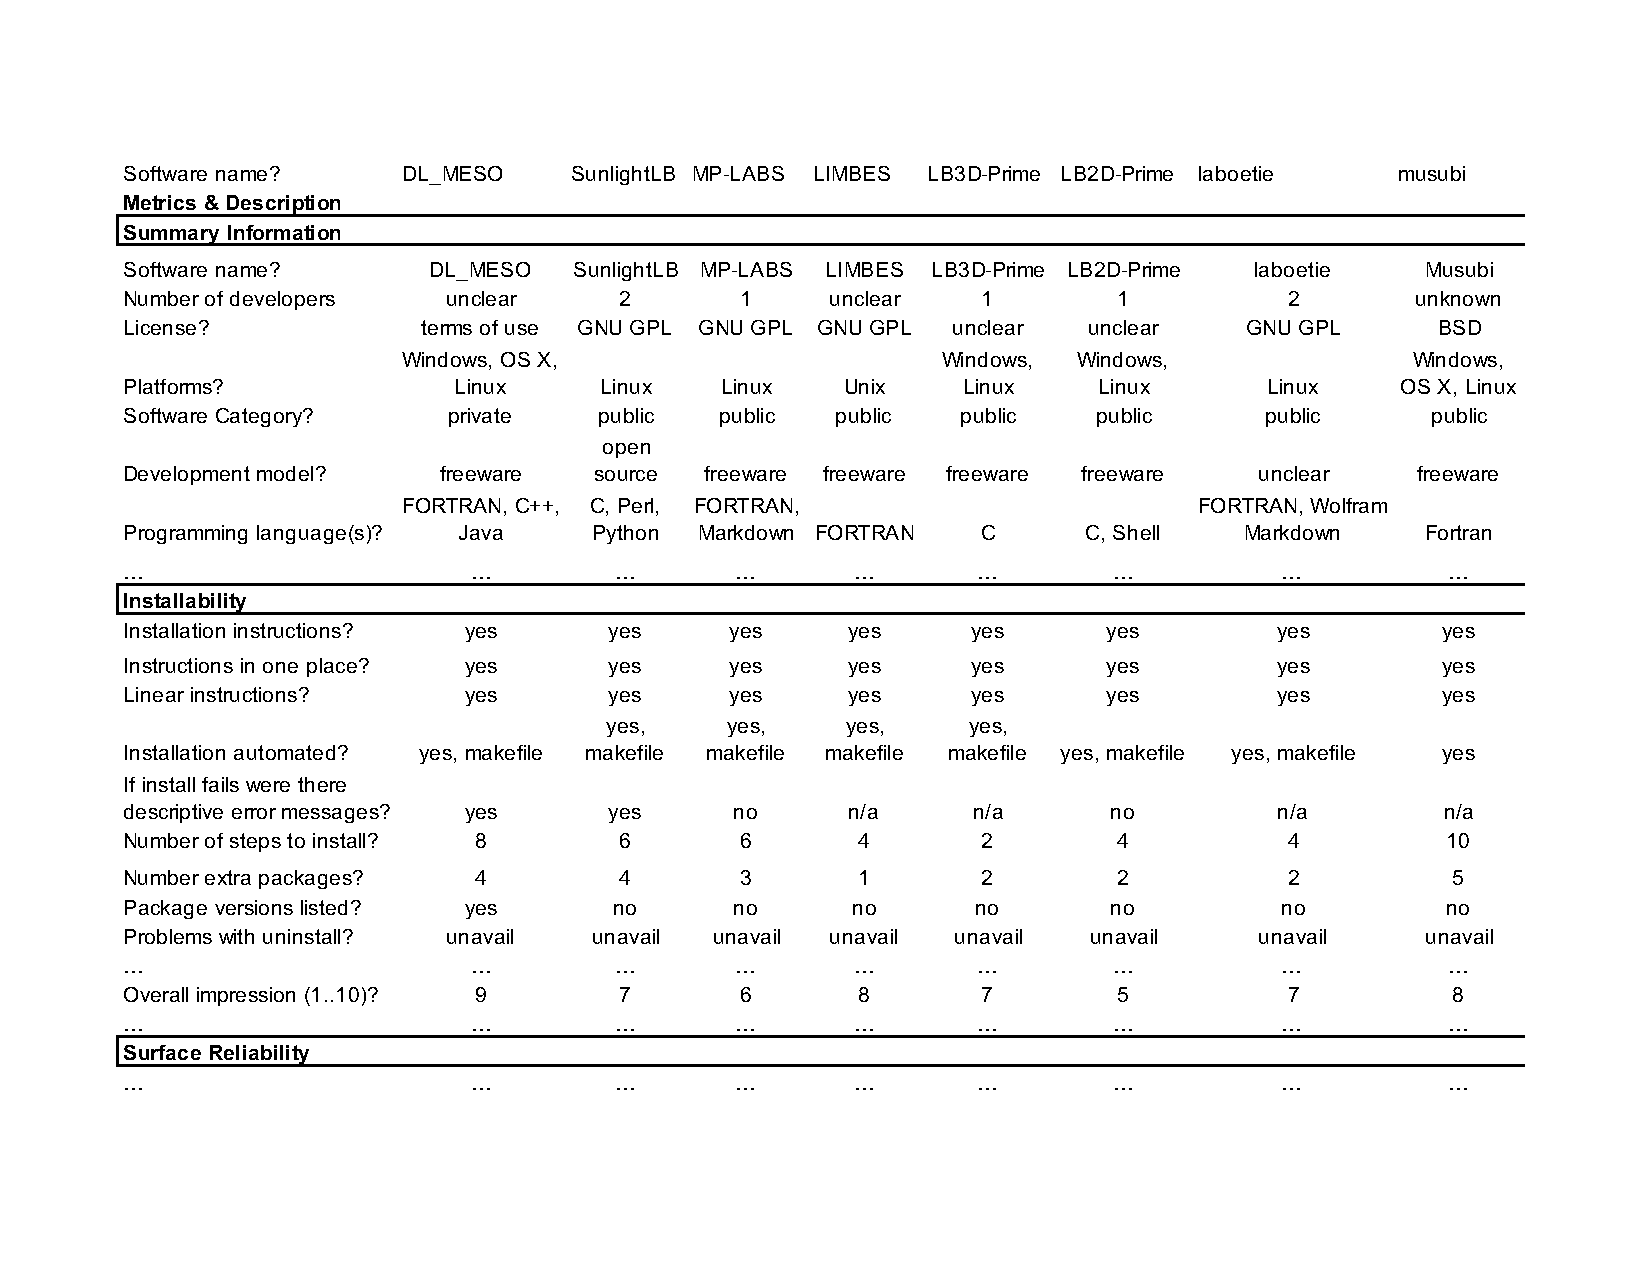
\includegraphics[width=1.0\textwidth]{./figures/measurement_template.pdf}
	  \caption{Excerpt of the Top Sections of the Measurement Template}
	  \label{measurement_template_image}
	\end{center}
\end{figure}

The full template consists of 108 questions categorized under nine qualities
(Section~\ref{softwarequalities}):
\begin{inparaenum}[(i)]
	\item installability;
	\item correctness and verifiability;
	\item surface reliability;
	\item surface robustness;
	\item surface usability;
	\item maintainability;
	\item reusability;
	\item surface understandability; and,
	\item visibility/transparency. 
\end{inparaenum} 

We designed the questions to be unambiguous, quantifiable, and measurable with
limited time and domain knowledge. We categorize them by quality, with an extra
category for summary information (Figure~\ref{measurement_template_image}). The
summary section provides general data, such as the software name, number of
developers, etc. \citet{gewaltig2012quality} provide us with our software
categories. Public means software available to all, while private means software
available only to a specific group.  The concept category defines software
written to demonstrate algorithms or concepts. The three categories of
development models are open source, where source code is freely available under
an open-source license; free-ware, which freely provides a binary or executable,
but not source code; and commercial, where the user must pay. 

Several of the qualities use the word ``surface'' to highlight that, for these
qualities, the best that we can do is a shallow measure. For instance, we do not
conduct experiments to measure usability directly. Instead, we look for
usability considerations by searching for cues in the documentation, such as the
presence of getting started instructions, a user manual, or documentation of
expected user characteristics. 

We used tools to automatically measure the number of files, number of lines of
code (LOC), percentage of closed issues, etc.
\href{https://github.com/tomgi/git_stats}{GitStats} \citep{Gieniusz2019}
measures each package's GitHub repository for the number of binary files, the
number of added and deleted lines, and the number of commits over varying time
intervals. \href{https://github.com/boyter/scc}{Sloc Cloc and Code (scc)}
\citep{Boyter2021} measures the number of text files and the number of total,
code, comment, and blank lines in each GitHub repository. 

As in \citet{SmithEtAl2016}, %DOUBLE BLIND
we used Virtual Machines (VMs) to provide an
optimal testing environment for each package. We used VMs to create fresh
environments, eliminating any worries about existing libraries and conflicts.
Moreover, when the tests are complete, the VM can be deleted, without impacting
the host operating system. The most significant advantage of using VMs is that
they level the playing field. Every software install starts from a clean slate,
which removes ``works-on-my-computer'' errors.

\subsection{Analytic Hierarchy Process} \label{AHP}

Once we measure each package, we still need to rank them to answer
\rqref{RQ_HighestQuality}. We do this via the Analytic Hierarchy Process (AHP)
\citep{Saaty1980}, a decision-making technique that compares multiple options by
multiple criteria. Our AHP algorithm uses the overall impression score, gathered
via the measurement template, \DIFdelbegin \DIFdel{to compare and }\DIFdelend \DIFaddbegin \DIFadd{along with pairwise comparisons between packages
to }\DIFaddend rank the LBM software. \DIFdelbegin \DIFdel{AHP performs a pairwise analysis using a matrix and generates an individual quality }\DIFdelend \DIFaddbegin \DIFadd{We have previously used this technique to rank
scientific software} 
\citep{SmithEtAl2016}.

\DIFadd{AHP focuses on relative comparisons, rather than requiring an unattainable
unified scale for measuring quality.  AHP starts with sets of $n$
}\textit{\DIFadd{options}} \DIFadd{and $m$ }\textit{\DIFadd{criteria}}.  In our project there are 24
software products ($n=24$) and 9 qualities ($m = 9$).  To get a ranking for each
criterion, we perform a pairwise analysis between each of the options, in the
form of an $n \times n$ matrix $A$.  The value of $A_{jk}$ ranges from 1 to 9,
using the following definitions 
\citep{Saaty1980}:

\begin{itemize}
\item \DIFadd{1 means equal importance. Two activities contribute equally to the
  objective.
}\item \DIFadd{3 means weak importance of one over another. Experience and judgment
  slightly favor one activity over another.
}\item \DIFadd{5 means essential or strong importance. Experience and judgment strongly
  favor one activity over another.
}\item \DIFadd{7 means demonstrated importance. An activity is strongly favored and its
  dominance demonstrated in practice.
}\item \DIFadd{9 means absolute importance. The evidence favoring one activity over
  another is of the highest possible order of affirmation.
}\item \DIFadd{2, 4, 6, 8 are defined as intermediate values between the two adjacent
  judgments.
}\end{itemize}

\DIFadd{During our grading process we capture a subjective score, from one to ten, for
each package for each criterion.  To turn these into Saaty's pair-wise scores
for option $x$ versus option $y$, we use the following calculation from the
respective subjective scores $x_{\text{sub}}$ and $y_{\text{sub}}$:
}\[
\DIFadd{\begin{cases}
\min\{9, x_{\text{sub}} - y_{\text{sub}} + 1\} & x_{\text{sub}} \geq y_{\text{sub}} \\
1 / \min\{9, y_{\text{sub}} - x_{\text{sub}} + 1\} & x_{\text{sub}} < y_{\text{sub}}
\end{cases}
}\]

\noindent \DIFadd{For example, we measured the installability for DL\_MESO and waLBerla 
as $9$ and $4$, respectively; therefore, on the 9-point scale, DL\_MESO compared to
waLBerla is 6 and waLBerla compared to DL\_MESO is 1/6, as shown in the sample
AHP calculations (Table~\ref{Tbl_SampleAHP}).
}

\DIFadd{In our work, we make the common assumption of a reciprocal relationship
between options $k$ and $j$; that is, $A_{kj}=1/A_{jk}$.  A partial view of $A$
for the quality of installability is found in Table~\ref{Tbl_SampleAHP}.  To
obtain the overall }\DIFaddend score for each \DIFaddbegin \DIFadd{option for a
given criterion we use matrix $B$, where $B_{jk} = A_{jk}/\sum_{i=1}^{i=n}(A_{i
k})$.  That is, to get $B$ we normalize the columns of $A$ by dividing by the
sum of the entries in the column, as shown in Table~\ref{Tbl_SampleAHP}.  For a
given quality, the score ($s_j$) for software package $j$ is found by averaging
the entries in row $j$ of $B$.  That is, $s_j = \frac{1}{n}
\sum_{i=1}^{i=n}(B_{j i})$, as shown in the final column of
Table~\ref{Tbl_SampleAHP}.  For the AHP method, the sum of the final $s_j$ values
for a given quality is 1.0.  Sorting the $s_j$ values provides a ranking for the
software packages for the quality under investigation.  The $s_j$ values can be
combined for all qualities for an overall ranking, as discussed in
Section~\ref{Sec_OverallQuality}. }\DIFaddend 

\DIFaddbegin \begin{table}[h!]
\begin{center}
\begin{tabular}{ l c c c c c | c c c c c | c }
 %DIF > \toprule
 \DIFaddFL{~ }& \multicolumn{5}{l}{A Matrix} & \multicolumn{5}{l}{BMatrix} & \DIFaddFL{~}\\
 \midrule
 \DIFaddFL{~ }& \rotatebox{90}{DL\_MESO} & \rotatebox{90}{waLBerla} & \rotatebox{90}{SunlightLB} & \DIFaddFL{$\cdots$ }& \rotatebox{90}{Musubi} & \rotatebox{90}{DL\_MESO} & \rotatebox{90}{waLBerla} & \rotatebox{90}{SunlightLB} & \DIFaddFL{$\cdots$ }& \rotatebox{90}{Musubi} & \DIFaddFL{AVG }\\
 \midrule
 \DIFaddFL{DL\_MESO (LBE) }& \DIFaddFL{1 }& \DIFaddFL{6 }& \DIFaddFL{3 }& \DIFaddFL{$\cdots$ }& \DIFaddFL{2 }& \DIFaddFL{0.0691 }& \DIFaddFL{0.0622 }& \DIFaddFL{0.0808 }& \DIFaddFL{$\cdots$ }& \DIFaddFL{0.0808 }& \DIFaddFL{0.072}\\
 \DIFaddFL{waLBerla }& \DIFaddFL{1/6 }& \DIFaddFL{1 }& \DIFaddFL{1/4 }& \DIFaddFL{$\cdots$ }& \DIFaddFL{1/5 }& \DIFaddFL{0.0115 }& \DIFaddFL{0.0104 }& \DIFaddFL{0.0067 }& \DIFaddFL{$\cdots$ }& \DIFaddFL{0.0067 }& \DIFaddFL{0.009}\\
 \DIFaddFL{SunlightLB }& \DIFaddFL{1/3 }& \DIFaddFL{4 }& \DIFaddFL{1 }& \DIFaddFL{$\cdots$ }& \DIFaddFL{1/2 }& \DIFaddFL{0.0230 }& \DIFaddFL{0.0415 }& \DIFaddFL{0.0269 }& \DIFaddFL{$\cdots$ }& \DIFaddFL{0.0269 }& \DIFaddFL{0.031}\\
 \DIFaddFL{$\vdots$ }& \DIFaddFL{$\vdots$ }& \DIFaddFL{$\vdots$ }& \DIFaddFL{$\vdots$ }& \DIFaddFL{$\ddots$ }& \DIFaddFL{$\vdots$ }& \DIFaddFL{$\vdots$ }& \DIFaddFL{$\vdots$ }& \DIFaddFL{$\vdots$ }& \DIFaddFL{$\ddots$ }& \DIFaddFL{$\vdots$ }& \DIFaddFL{$\vdots$}\\
 \DIFaddFL{Musubi }& \DIFaddFL{1/2 }& \DIFaddFL{5 }& \DIFaddFL{2 }& \DIFaddFL{$\cdots$ }& \DIFaddFL{1 }& \DIFaddFL{0.0345 }& \DIFaddFL{0.0518 }& \DIFaddFL{0.0539 }& \DIFaddFL{$\cdots$ }& \DIFaddFL{0.0539 }& \DIFaddFL{0.048}\\  
 \midrule
 \DIFaddFL{SUM = }& \DIFaddFL{14.48 }& \DIFaddFL{96.50 }& \DIFaddFL{37.12 }& \DIFaddFL{$\cdots$ }& \DIFaddFL{23.78 }& \DIFaddFL{1.000 }& \DIFaddFL{1.000 }& \DIFaddFL{1.000 }& \DIFaddFL{$\cdots$ }& \DIFaddFL{1.000 }& \DIFaddFL{1.000}\\
 \bottomrule
\end{tabular}
\end{center}
\caption{\DIFaddFL{Sample AHP Calculations for the Quality of Installability}} \label{Tbl_SampleAHP}
\end{table}

\DIFaddend We use our own simple tool for conducting the AHP analysis. The tool includes a
sensitivity analysis to ensure that the software package rankings are
appropriate with respect to the uncertainty of the quality scores. For the
sensitivity analysis, we modified the score by 10\% for each package and
verified that the overall ranking was stable.  
The
\href{https://github.com/smiths/AIMSS/blob/master/StateOfPractice/AHP2020/LBM/README.txt}{README}
file for the tool includes requirements and usage information. %DOUBLE BLIND

\subsection{Interview Developers} \label{SecSurvey}

Two of the research question (\rqref{RQ_PainPoints} and \rqref{RQ_Concerns})
require going beyond the quantitative data from the measurement template. To
gain insight, we interview developers using a list of 20 questions from 
\citet{SmithEtAl2021}. %DOUBLE BLIND
The questions cover the background of the development
teams, the interviewees, and the software itself. We ask the developers how they
organize their projects and about their understanding of the users. Some
questions focus on the current and past difficulties, and the solutions the team
has found or will try. We also discuss the importance of, and the current
situation for, documentation. A few questions focus on specific software
qualities, such as maintainability, understandability, usability, and
reproducibility. The interviews are semi-structured based on the question list;
we ask follow-up questions when necessary. Based on our experience, the
interviewees often raise exciting and unexpected ideas.

We requested interviews with developers for all 24 packages, except Musubi,
since we added Musubi after our ethics approval expired. We found the developers
from project websites, code repositories, publications, and biographic
information on institution webpages. Four developers agreed to participate in
our study. We met with them online, using either Zoom or Teams to facilitate
recording and automatic transcription. Each meeting lasted about an hour. 
The
McMaster University Research Ethics Board approved the interview process under
application number
\href{https://github.com/smiths/AIMSS/blob/master/StateOfPractice/MACREM/Application.pdf}
{MREB\#: 5219}. %DOUBLE BLIND

\subsection{Domain Analysis} \label{SecDomainAnalysis}

Since the LBM domain has a reasonably small scope, we can view the software as
constituting a program family.  \citet{parnas1976design} defines a program
family as ``a set of programs whose common properties are so extensive that it
is advantageous to study the common properties of the programs before analyzing
individual members.'' Domain analysis is the term for studying the common
properties within a family of related programs.

The domain analysis (also called a commonality analysis) consists of
understanding the commonalities, variabilities, and common terminology for a
program family \citep{weiss1997defining}. Commonalities are goals, theories,
models, definitions, and assumptions that are common between family members.
Variabilities are goals, theories, models, definitions, and assumptions that
differ between family members. Associated with each variability are parameters
of variation, which summarize the possible values for that variability, along
with their potential binding time. The binding time is when a variability is
assigned a value. Binding time options include specification time, build time
(when the program compiles) and run time (when the code executes). For the
current assessment, the packages all have the commonality of using LBM
techniques to simulate the motion of fluids. Variabilities for LBM packages
include the following: the dimension of problems they simulate, whether (and
how) they support parallel computation, whether compressibility can be
considered, whether reflexive boundaries can be employed, whether the simulation
handles multi-fluids, whether the simulation handles turbulence, and whether
complex geometries can be simulated. 

To focus the current presentation, we only present the results of our shallow
domain analysis. We distinguish programs by their variabilities, which for
research software are often assumptions. Table~\ref{tbl_features}, which is
sorted alphabetically, lists the variabilities as columns. \citet{Michalski2021}
provides a more detailed analysis of the commonalities and variabilities between
LBM packages.

\begin{table}[ht!]
	\begin{center}
		\begin{tabular}{ p{3cm}llllllll}
			\toprule
			Name & Dim & Pll & Com & Rflx & MFl & Turb & CGE & OS\\
			\midrule
			DL\_MESO (LBE) & 2, 3 & MPI/OMP & Y & Y & Y & Y & Y & W, M, L\\
			ESPResSo & 1, 2, 3 & CUDA/MPI & Y & Y & Y & Y & Y & M, L\\
			\esp{} & 1, 2, 3 & MPI & Y & Y & Y & Y & Y & L\\
			HemeLB & 3 & MPI & Y & Y & Y & Y & Y & L\\
			laboetie & 2, 3 & MPI & Y & Y & Y & Y & Y & L\\
			LatBo.jl & 2, 3 & — & Y & Y & Y & N & Y & L\\
			LB2D-Prime & 2 & MPI & Y & Y & Y & Y & Y & W, L\\
			LB3D & 3 & MPI & N & Y & Y & Y & Y & L\\
			LB3D-Prime & 3 & MPI & Y & Y & Y & Y & Y & W, L\\
			lbmpy & 2, 3 & CUDA & Y & Y & Y & Y & Y & L\\
			lettuce & 2, 3 & CUDA & Y & Y & Y & Y & Y & W, M, L\\
			LIMBES & 2 & OMP & Y & Y & N & N & Y & L\\
			Ludwig & 2, 3 & MPI & Y & Y & Y & Y & Y & L\\
			LUMA & 2, 3 & MPI & Y & Y & Y & Y & Y & W, M, L\\
			MechSys & 2, 3 & — & Y & Y & Y & Y & Y & L\\
			MP-LABS & 2, 3 & MPI/OMP & N & Y & Y & N & N & L\\
			Musubi & 2, 3 & MPI & Y & Y & Y & Y & Y & W, L\\
			OpenLB & 1, 2, 3 & MPI & Y & Y & Y & Y & Y & W, M, L\\
			Palabos & 2, 3 & MPI & Y & Y & Y & Y & Y & W, L\\
			pyLBM & 1, 2, 3 & MPI & Y & Y & N & Y & Y & W, M, L\\
			Sailfish & 2, 3 & CUDA & Y & Y & Y & Y & Y & M, L\\
			SunlightLB & 3 & — & Y & Y & N & N & Y & L\\
			TCLB & 2, 3 & CUDA/MPI & Y & Y & Y & Y & Y & L\\
			waLBerla & 2, 3 & MPI & Y & Y & Y & Y & Y & L\\
			\bottomrule
		\end{tabular}
		\caption{Features of Software Packages (Dim for Dimension (1, 2, 3), Pll
			for Parallel (CUDA, MPI, OpenMP (OMP)), Com for Compressible (Yes or
			No), Rflx for Reflexive Boundary Condition (Yes or No), MFl for
			Multi-fluid (Yes or No), Turb for Turbulent (Yes or No), CGE for
			Complex Geometries (Yes or No), OS for Operating System (Windows
			(W), macOS (M), Linux (L))) (Sorted Alphabetically)} \label{tbl_features}
	\end{center}
\end{table}

\subsection{Interaction With Domain Expert} \label{sec_vet_software_list}

We partnered with a Domain Expert to vet our list of projects
(\rqref{RQ_WhatProjects}) and our ranking (\rqref{RQ_HighestQuality}). The
Domain Expert is a crucial member of the state of the practice assessment team.
Pitfalls exist if non-experts attempt to acquire an authoritative list of
software or try to rank the software. Non-experts rely on online information,
which has the following drawbacks:
\begin{inparaenum}[i)]
  \item the online resources could have false or inaccurate information, and 
  \item the online resources could leave out relevant information that is too
  ingrained with experts for them to explicitly record it.
\end{inparaenum}
For the current assessment, our Domain Expert (and paper co-author) is Dr.\
 Zahra Keshavarz-Motamed, Assistant Professor of Mechanical Engineering at
McMaster University, Hamilton, Ontario, Canada.  

The Domain Expert has a central role in verifying the list of packages. In
advance of the first meeting with the Domain Expert, we ask them to create a
list of top software packages in the domain.  We do this to help the expert get
in the right mindset for our meeting.  Moreover, by doing the exercise in
advance, we avoid the potential pitfall of the expert approving the discovered
list of software without giving it adequate thought. We ask the Domain Expert to
vet the collected data and analysis. In particular, we ask them to vet the
proposed list of software packages and the AHP ranking.

\section{Ranking Projects Based on Quality Measures} \label{AHPresults}

We answer \rqref{RQ_HighestQuality} by using AHP to rank the identified LBM
software against best practices.  The sections below summarize how the software
packages compare based on the qualities discussed in
Section~\ref{softwarequalities}, as measured via the measurement template
(Section~\ref{empiricalmeasures}).  The last subsection combines all the
qualities into one ``global'' ranking.  The full LBM data is available publicly
on Mendeley Data \citep{Smith2022}. %DOUBLE BLIND

\subsection{Installability}

All 24 software packages have installation instructions. Most have their
installation instructions located in one place, often in an instruction manual
or a webpage. Sometimes, like with Ludwig, we found incomplete installation
instructions in one place, but complete instructions elsewhere. Installability
of the software, and maintainability and correctness of the instructions
themselves, are improved if all the instructions are in one location.

All 24 packages are installable on a Unix-like system. Eight packages are also
installable on Windows, and five on macOS. Twenty packages list their operating
system requirements, but only four (ESPResSo, LUMA, Mechsys, Sailfish) list
compatible operating system versions. Ubuntu provided the testing platform for
all packages, except for TCLB, which we tested on CentOS, as suggested by its
installation instructions. 

All but one of the software packages (LatBo.jl) have automated at least part of
the installation process. Most packages, such as waLBerla and SunlightLB, use
Make to automate the installation, and a few of them, like lbmpy, use custom
scripts.

In most of the cases with installation errors, descriptive error messages
allowed us to proceed. Systems that provided vague error messages, such as
messages that did not specify which action or file was at fault, were harder to
troubleshoot. Only three software packages (HemeLB, LB3D, lbmpy) that displayed
a descriptive error message were not recoverable, and most of these instances
were due to hardware and operating system incompatibility, such as the
requirement of CUDA. Fourteen software packages broke during installation. Some
packages, such as LB2D-Prime and LB3D-Prime did not provide a definitive message
of the success or failure of the installation. In these instances, validating
the installation required performing a tutorial or running a script, if these
were available. 

About half of the installation instructions assume the user is already aware of,
and has already installed, dependent packages. Many packages, like \esp, Ludwig
and LUMA, do not list all their dependencies. Sometimes only an error message
during the installation process informs the user of a required dependency. In
cases like this, we suggest a detailed rewrite of the installation instructions
to accommodate a clean operating system. A virtual machine can provide an
environment for installability testing.

Seventeen software packages require installation of less than 10 dependencies.
All software package (except for LatBo.jl) require less than 20 dependencies.
Some packages may automatically install additional dependencies in the
background. Twenty of the software packages do not explicitly indicate the
versions of software dependencies. Some software package installation issues
could have been avoided by providing a list of dependencies. Sixteen software
packages do not have detailed instructions for installing dependencies. Sixteen
software packages have less than 10 manual installation steps. If one command
installs dependencies, then none of the software packages take more than 20
steps to install. The average number of steps is eight, and the fewest is two
(LB3D-Prime).

All but six (ESPResSo, HemeLB, laboetie, LB3D-Prime, lbmpy, waLBerla) of the
software packages have a way to verify the installation. Most have tutorial
examples for the user to run. Some other approaches to installation validation
include validation scripts (LB2D-Prime, lettuce, Ludwig, LUMA), automatic
validation after the installation (LatBo.jl), and instructions to manually
review the file system (LIMBES). Only one software package (pyLBM) has
uninstallation instructions.

\begin{figure}[h!]
	\begin{center}
		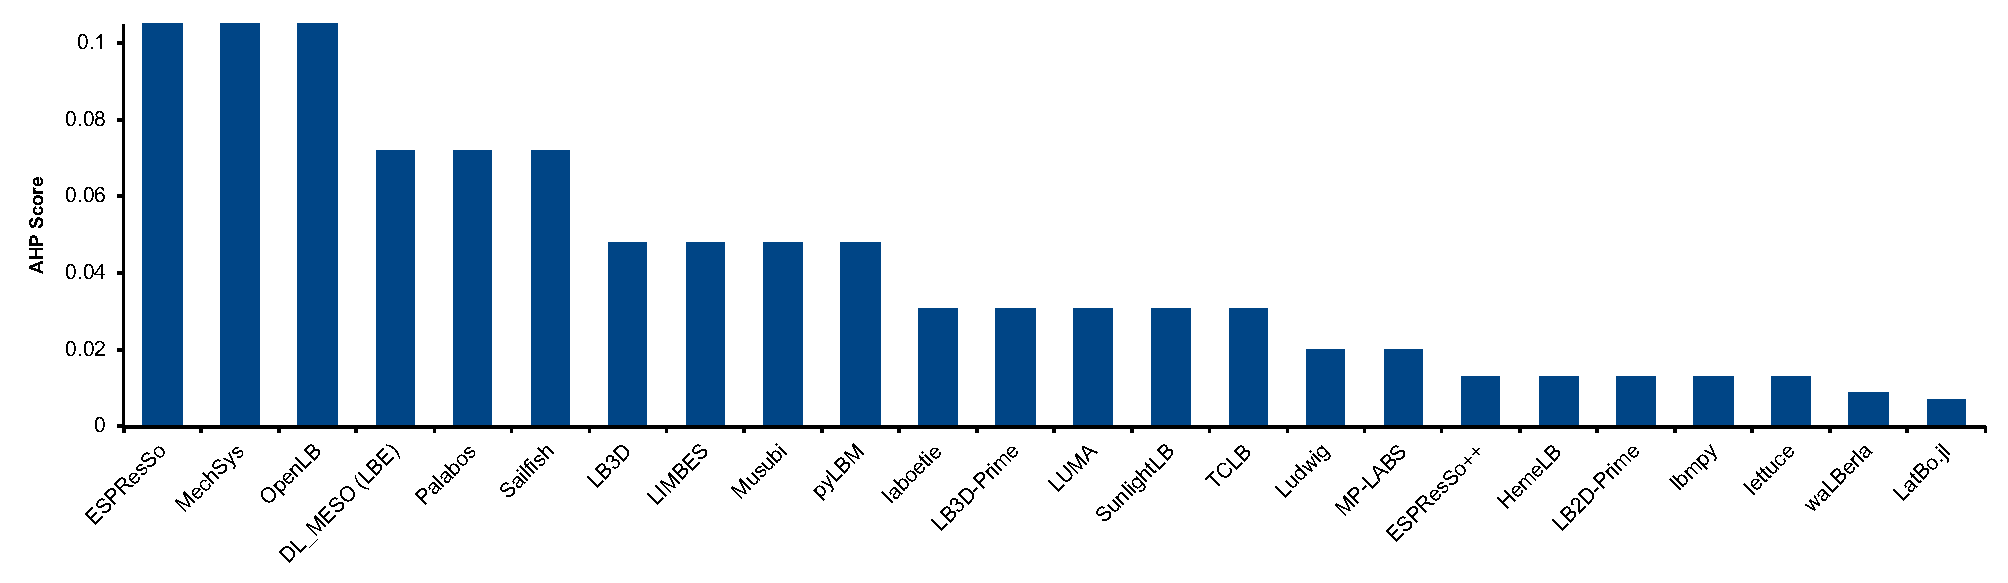
\includegraphics[width=1.0\textwidth]{./figures/installability_chart.pdf}
		\caption{AHP Installability Score}
		\label{Fig_Installability}
	\end{center}
\end{figure}

Figure~\ref{Fig_Installability} shows the installability ranking of the software
packages. Software packages with a higher score (ESPResSo, MechSys, OpenLB,
DL\_MESO, Palabos\DIFaddbegin \DIFadd{, Sailfish}\DIFaddend ) tend to have one set of linear installation
instructions, written as if the person doing the installation has none of the
dependencies installed. The instructions often list compatible operating system
versions and include instructions for installing dependencies. The top-ranked
packages often incorporate some automation of the installation process. The
number of dependencies a package has does not correlate with a higher score. The
ability to validate the installation process, say through tutorials or test
cases, leads to a higher score. Apparently active work on a project improves
installability since the top \DIFdelbegin \DIFdel{seven }\DIFdelend \DIFaddbegin \DIFadd{six }\DIFaddend ranked packages are all classified as alive. 

\subsection{Surface Correctness and Verifiability} \label{SecSurfCorrectAndVerifiab}

Seventeen software packages explicitly reference domain theory, but a complete
and rigorous requirements specification, in the software engineering sense
\citep{IEEE1998, RobertsonAndRobertson1999Vol, ESA1991}, is absent from all
projects. Software packages that include a subset of a requirements
specification, such as DL\_MESO (LBE), keep the information brief and include it
within other documents, such as a user manual, webpage, or a publication. In the
latter case tracking down the knowledge may take significant time. 

Thirteen software packages explicitly use document generation tools. Eight of
them use Sphinx and the same number use Doxygen. Several packages use both.

Tutorials are available for 19 of the packages. Generally they are linearly
written and easy to follow. However, only eight tutorials provide expected
outputs, making it difficult to verify the correctness of their output. In these
cases the user may need to assume correctness if there are no visible errors.
\href{https://www.walberla.net/doxygen/index.html} {waLBerla} provides a
particularly detailed tutorial, including expected output.

Unit tests are only explicitly available for two of the software packages,
Ludwig and Musubi. Code modularization of most packages allows for users to
create tests with varying degrees of effort. These tests allow developers and
users to verify the correctness of fragments of the source code, and in doing so
better assess the correctness of the entire package.

The use of Continuous Integration (CI) tools and techniques alludes to a refined
development process that quickly isolates and fixes faults. Only three of the
packages (ESPResSo, Ludwig, Musubi) mentioned applying the practice of CI in
their development process.

\begin{figure}[h!]
	\begin{center}
		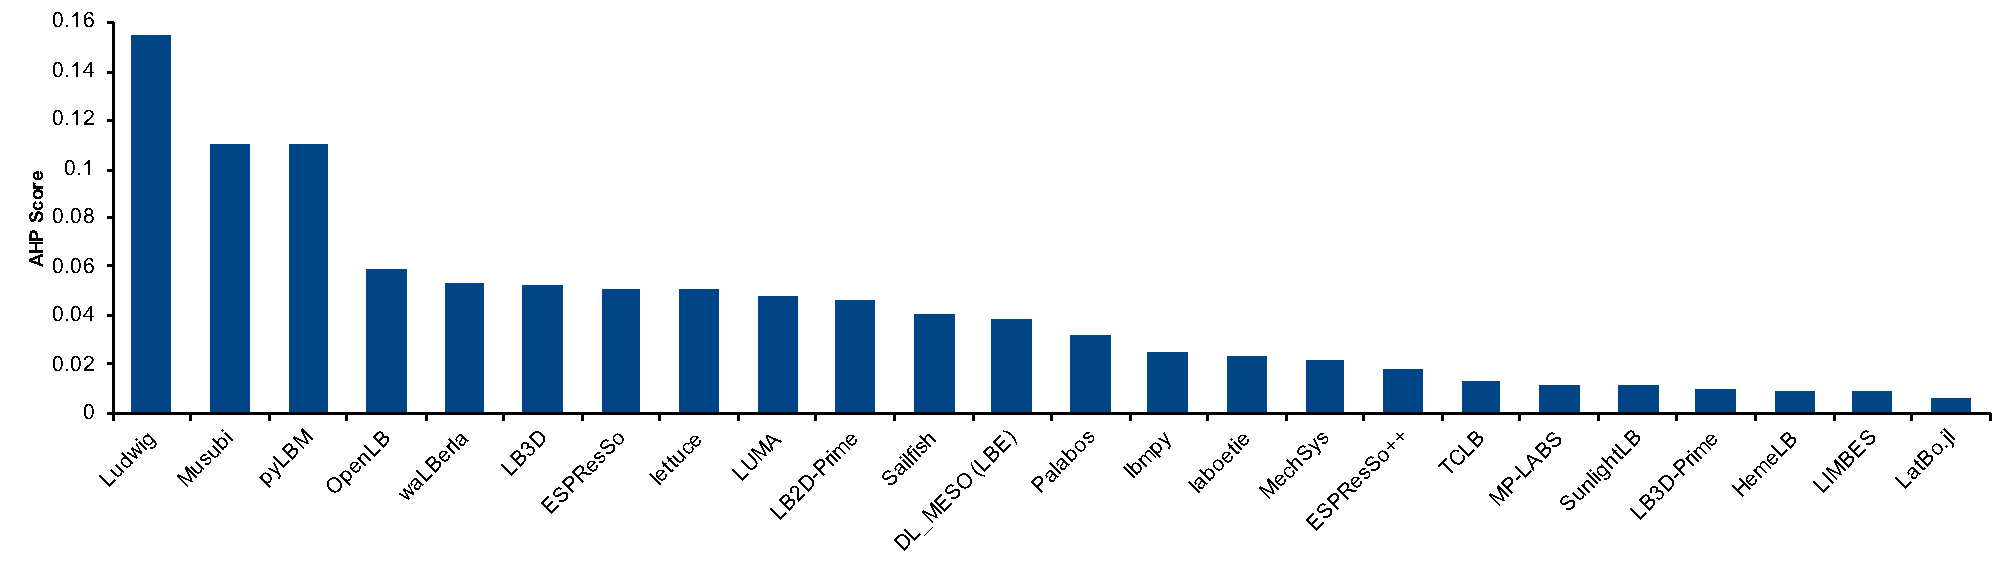
\includegraphics[width=1.0\textwidth]{./figures/correctnessverifiability.pdf}
		\caption{AHP Surface Correctness and Verifiability Score}
		\label{Fig_CorrectnessVerifiability}
	\end{center}
\end{figure}

Figure~\ref{Fig_CorrectnessVerifiability} shows the ranking for surface
correctness and verifiability. Software packages with a higher score tend to
have theory documentation. They also explicitly use at least one document
generation tool that helps with verification, thus building confidence in
correctness. The top ranked software packages all include getting started
tutorials, and most of these include expected output. \DIFdelbegin \DIFdel{The two }\DIFdelend \DIFaddbegin \DIFadd{Two of the }\DIFaddend top ranked
packages, Ludwig and Musubi, indicate the use of unit testing in their
documentation. They also incorporated CI in the development process.
Furthermore, \DIFdelbegin \DIFdel{eight of the top 10 }\DIFdelend \DIFaddbegin \DIFadd{all the top 5 }\DIFaddend ranked packages are alive.

\subsection{Surface Reliability}

The analysis of surface reliability focuses on package installation and
tutorials. Errors occurred when installing 16 of the software packages. Every
instance prompted an error message. These messages indicated unrecognized
commands (even when following the installation guide), missing links, missing
dependencies, and syntax errors in code files. In some instances the error
messages were vague. Several automatic installation processes could not find or
load dependencies. In these instances the installation tried to access outdated
external repositories. We recovered and verified seven of the installations, and
we assumed that one of the installations (LB3D-Prime) was recovered, since there
was no way to test the installation. The installation of eight of the software
packages could not be recovered. Most of these broken installations could not
find external dependencies, encountered system incompatibilities, or displayed
vague error messages.

Of the 14 software packages that installed correctly and also have tutorials,
four (pyLBM, \esp, LIMBES, Ludwig) broke during tutorial testing. All of these
instances resulted in the display of an error message. One error (pyLBM) was due
to a missing tutorial dependency, another (Ludwig) was due to an invalid command
despite following the tutorial, and the final two errors were vague execution
errors. Of the four broken tutorial instances, only the one due to a missing
dependency was recoverable. 

\begin{figure}[h!]
	\begin{center}
		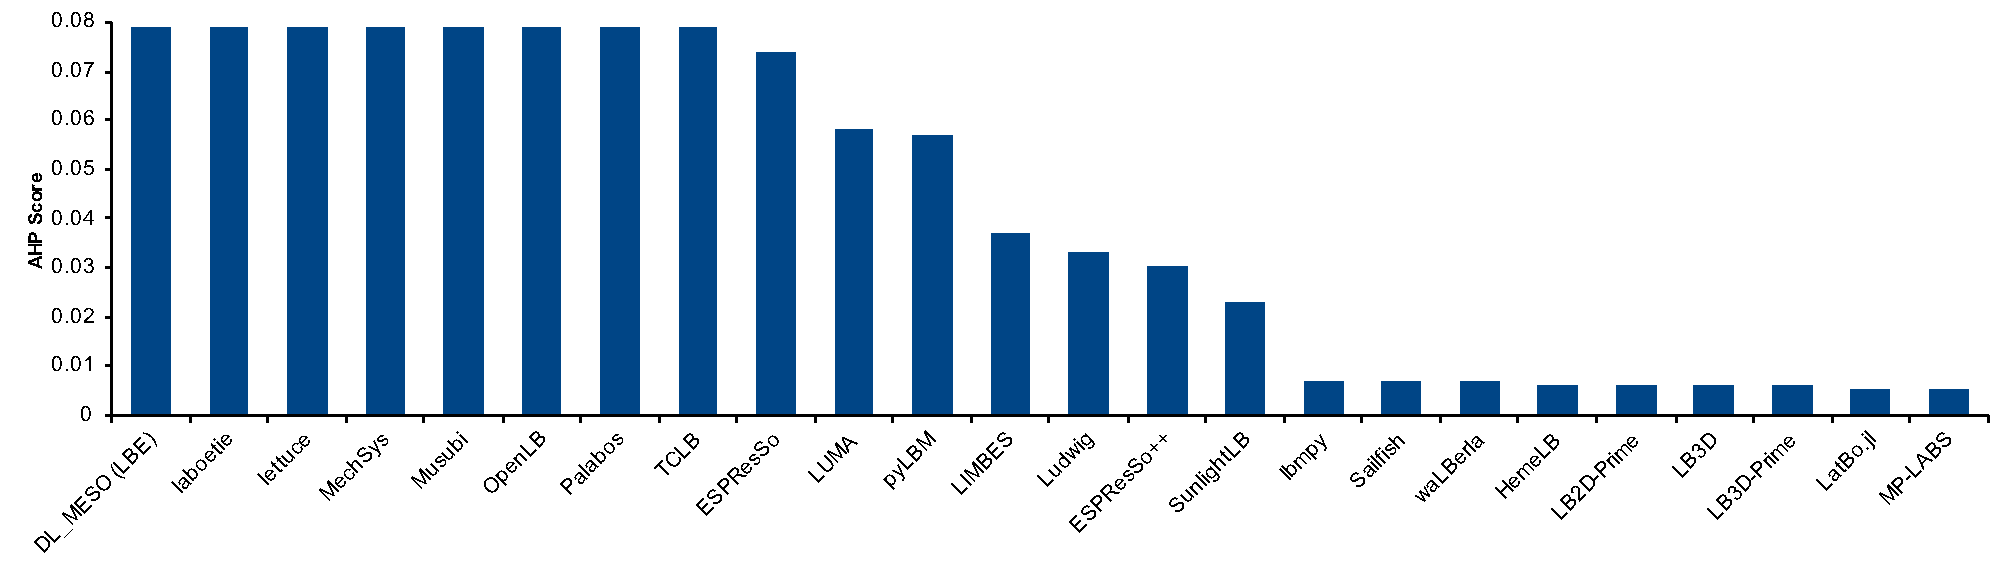
\includegraphics[width=1.0\textwidth]{./figures/reliability_chart.pdf}
		\caption{AHP Surface Reliability Score}
		\label{Fig_Reliability}
	\end{center}
\end{figure}

Figure~\ref{Fig_Reliability} shows the surface reliability ranking of the
software packages. Software packages with a high score either did not break
during installation, or the broken installation was recoverable. \DIFdelbegin \DIFdel{All the top
five ranked packages have tutorials. }\DIFdelend The package
pyLBM broke during tutorial testing, but a descriptive error message helped in
recovery. \DIFdelbegin \DIFdel{Nine }\DIFdelend \DIFaddbegin \DIFadd{Ten }\DIFaddend of the top \DIFdelbegin \DIFdel{10
}\DIFdelend \DIFaddbegin \DIFadd{11 }\DIFaddend packages are alive. 

\subsection{Surface Robustness} \label{Sec_Robustness}

Robustness testing includes handling unexpected input, such as incorrect data
types, empty input, and missing files or links. A reasonable response, including
appropriate error messages and an absence of unrecoverable system failures,
means success. 

\begin{figure}[h!]
	\begin{center}
		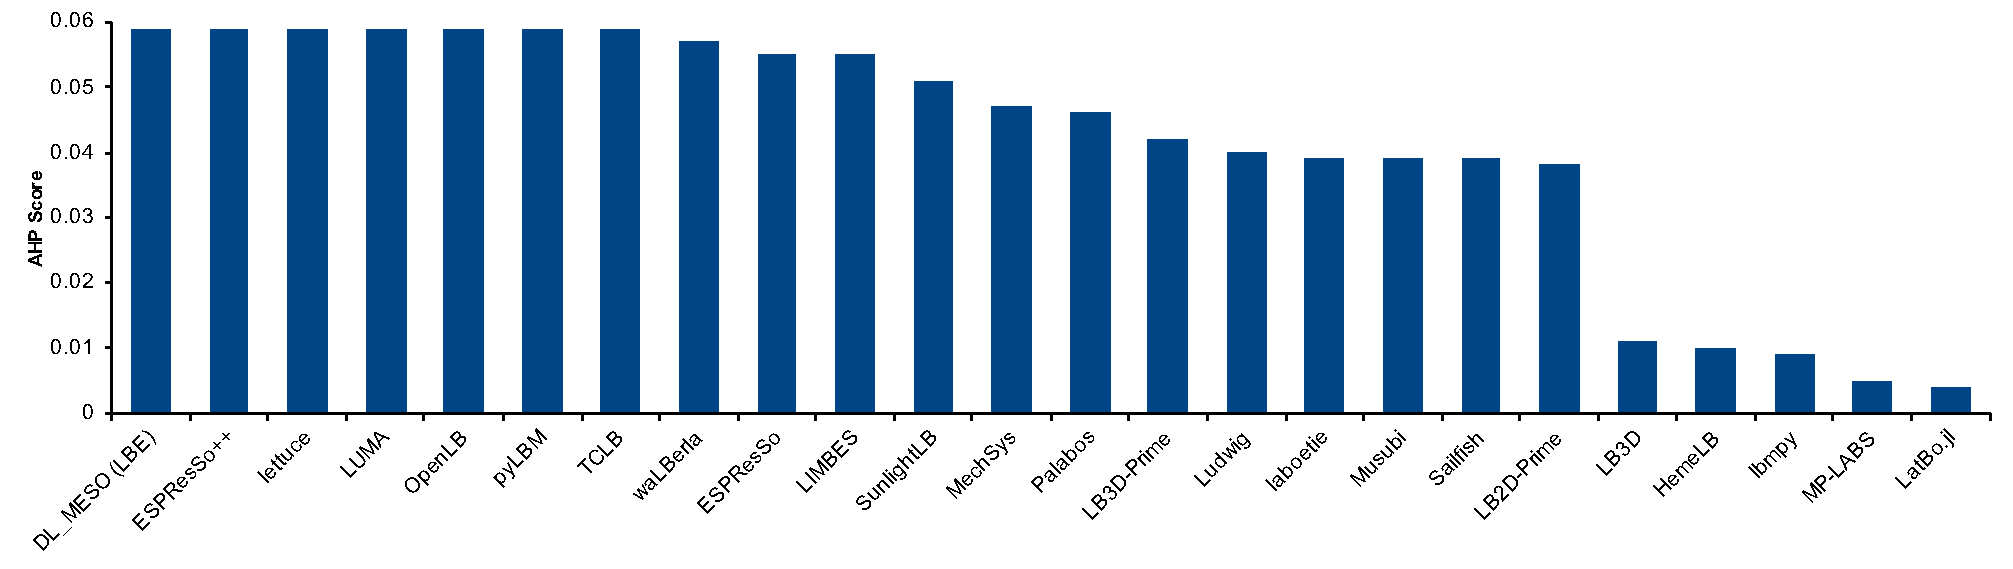
\includegraphics[width=1.0\textwidth]{./figures/robustness_chart.pdf}
		\caption{AHP Surface Robustness Score}
		\label{Fig_Robustness}
	\end{center}
\end{figure}

Figure~\ref{Fig_Robustness} shows the surface robustness ranking of the software
packages. Software packages with a high score behaved reasonably in response to
unexpected input as described above. All the software packages that installed
correctly passed this test. They did not crash and usually output descriptive
error messages. Software packages with a lower surface robustness score did not
install correctly, so their robustness score may not be a true reflection of
their runtime robustness. All successfully installed software packages that
require a plain text input file correctly handled an unexpected change to these
input files, including a replacement of new lines with carriage returns.
\DIFdelbegin \DIFdel{Following the trend of the other qualities, nine of the top 10 ranked packages
are alive.
}\DIFdelend 

\subsection{Surface Performance}

Although the software packages all apply LBM to solve scientific computing
problems, they differ in scope and capabilities, as shown in
Table~\ref{tbl_features}. Therefore, tests to compare run-time performance are
not appropriate. Instead, we look through each software package's artifacts
for evidence of considering performance. The artifacts of 18 software packages
mentioned parallelization. This included GPU processing and the CUDA parallel
computing platform, which were mentioned in the artifacts of six packages
(ESPResSo, lbmpy, lettuce, pyLBM, Sailfish, TCLB). When a high degree of
parallelization is possible, GPUs provide superior speed compared to CPUs. The
software package TCLB is implemented in a highly efficient multi-GPU code to
achieve performance suitable for model optimization \citep{rutkowski2020open}.
The Ludwig package uses a so-called mixed mode approach implementing
fine-grained parallelism on the GPU.  MPI is used for even larger scale
parallelism \citep{gray2013ludwig}. While one software package (Sailfish)
required CUDA and GPU processing, some (ESPResSo, lbmpy, lettuce, pyLBM, TCLB)
have the option of using either the GPU or the CPU. In general, the packages
that require GPU and CUDA have better performance at the expense of
installability and surface reliability.

\subsection{Surface Usability}

We review software repositories for the presence of a tutorial, a user manual,
documented user characteristics, and a user support model. In total 19 software
packages have a tutorial, 13 have a user manual, and 11 have both. The tutorials
vary in scope and substance, and eight include expected output. Most user
manuals are in the form of a file that can be downloaded, while some are
rendered on a webpage. Some packages (waLBerla) do not have a user manual, but
do have useful documentation distributed throughout their webpages. Five
software packages (laboetie, LIMBES, Ludwig, Musubi, Palabos) document expected
user characteristics. Users are typically scientists or engineers. Their
background is often physics, chemistry, biophysics, or mathematics. All projects
(except LIMBES) have a user support model, and many of them have multiple
avenues of user support. The most popular avenue of support is Git, followed by
email and forums. One software package (OpenLB) has an FAQ (Frequently Asked
Questions) page.    

\begin{figure}[h!]
	\begin{center}
		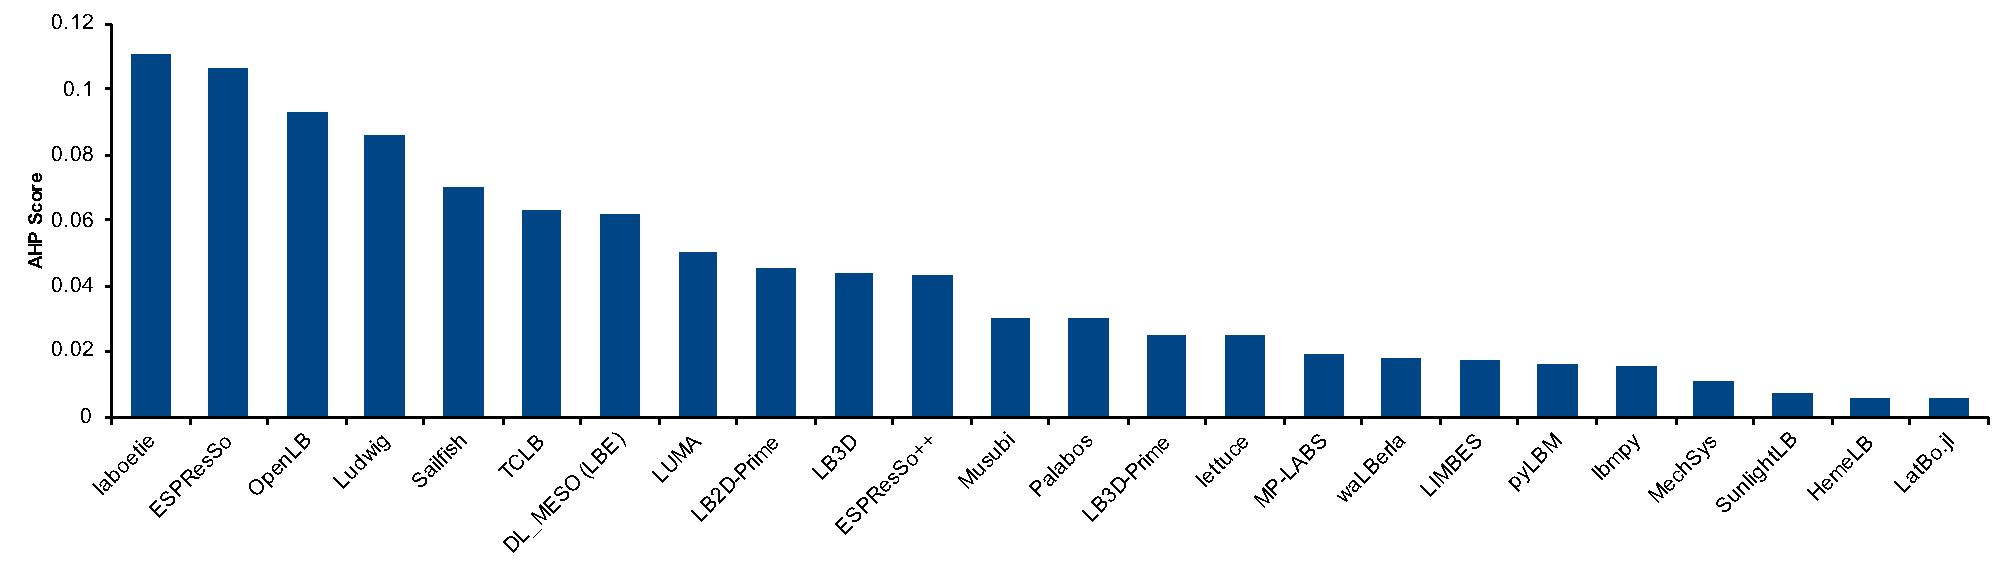
\includegraphics[width=1.0\textwidth]{./figures/usability_chart.pdf}
		\caption{AHP Surface Usability Score}
		\label{Fig_Usability}
	\end{center}
\end{figure}

Figure~\ref{Fig_Usability} shows the surface usability ranking of the software
packages. Software packages with a high score have a tutorial and user manual,
sometimes have documented user characteristics, and have at least one user
support model. Many packages have several user support models. Furthermore, four
of the top five packages are alive. 

\subsection{Maintainability} \label{Sec_Maintainability}

We review software packages for the presence of artifacts and recorded every
type of artifact that is not a code file. (The artifacts will be discussed
further in Section~\ref{Sec_CompareArtifacts}.)  We also reviewed the software
packages for software release and documentation version numbers. This
information can be used to troubleshoot issues and organize documentation. All
but three software packages (LatBo.jl, LB3D-Prime, MechSys) have source code
release and documentation version numbers.

We look for evidence that teams review code and have information on how users
can contribute. In total, 11 software packages have this information, found in
various artifacts, including in developer guides, contributor guides, user
guides, developer webpages, and README files. 

Twenty-three packages use issue tracking, 15 of which use GitHub or GitLab to
host their git repository, seven use email, and one (SunlightLB) uses
SourceForge. Most software packages that use GitHub or GitLab have the majority
of their issues closed, and only three (laboetie, lettuce, Sailfish) have less
than 50\% of their issues closed. All the top \DIFdelbegin \DIFdel{five }\DIFdelend \DIFaddbegin \DIFadd{four }\DIFaddend ranked packages have most of
their issues closed. Alive packages (11 use issue tracking) have 64\% of their
issues closed, while dead packages (3 use issue tracking) have 71\% of their
issues closed. Table~\ref{gitrepodata} presents this information. With respect
to the host for the git repository, 13 packages use GitHub and two (Palabos,
waLBerla) use GitLab. Of the other packages, one package (SunlightLB) uses CVS
for issue tracking and version control, and seven do not appear to use any issue
tracking system.  Assuming the use of GitHub, GitLab or CVS implies the use of
version control, 16 of 24 (67\%) of projects use version control.

\begin{table}[ht!]
	\begin{center}
		\begin{tabular}{ p{3.5cm}p{3.5cm}p{3.5cm}p{2.5cm} }
			\toprule
			Name & $\%$ Code Comments & $\%$ Issues Closed & Status\\
			\midrule
			MP-LABS & 26.67 & 100.00 & Dead\\
			Musubi & 24.19 & Not Git & Alive\\
			waLBerla & 22.62 & 72.90 & Alive\\
			OpenLB & 22.43 & Not Git & Alive\\
			ESPResSo & 21.78 & 89.26 & Alive\\
			Ludwig& 20.70 & 60.00 & Alive\\
			Palabos & 17.76 & 89.47 & Alive\\
			SunlightLB & 17.67 & Not Git & Dead\\
			LIMBES & 17.39 & Not Git & Dead\\
			\esp & 17.10 & 66.28 & Alive\\
			HemeLB & 16.68 & No Issues & Dead\\
			pyLBM & 16.12 & 66.67 & Alive\\
			MechSys & 15.11 & Not Git & Alive\\
			LB3D-Prime & 14.34 & Not Git & Dead\\
			LB3D & 13.76 & Not Git & Dead\\
			LB2D-Prime & 13.61 & Not Git & Dead\\
			Sailfish & 9.26 & 22.22 & Alive\\
			lettuce & 8.19 & 33.33 & Alive\\
			DL\_MESO (LBE) & 8.06 & Not Git & Alive\\
			TCLB & 6.02 & 60.32 & Alive\\
			laboetie & 2.47 & 18.75 & Dead\\	
			lbmpy& 2.03 & 58.33 & Alive\\	
			LatBo.jl & 0.40 & 93.33 & Dead\\
			LUMA& 0.20 & 85.71 & Alive\\
			\bottomrule
		\end{tabular}
		\caption{Git Repository Data, Sorted by Percentage of Code that is
			Comments (Sorted by $\%$ Code Comments)} \label{gitrepodata}
	\end{center}
\end{table}

Table~\ref{gitrepodata} shows the percentage of code that is comments, in
decreasing order. We assume maintainability improves for packages with a higher
percentage of comments. Comments represent more than 10\% of code files in 16
packages, and the average percentage of code comments is about 14\%. All the top
\DIFdelbegin \DIFdel{five }\DIFdelend \DIFaddbegin \DIFadd{four }\DIFaddend overall ranked packages have more than the average. LUMA has only 0.2\%
comments, the fewest of any package. However, this package also has the most
lines of source code, with over four million. The next largest package is \esp{}
with one million.

\begin{figure}[h!]
	\begin{center}
		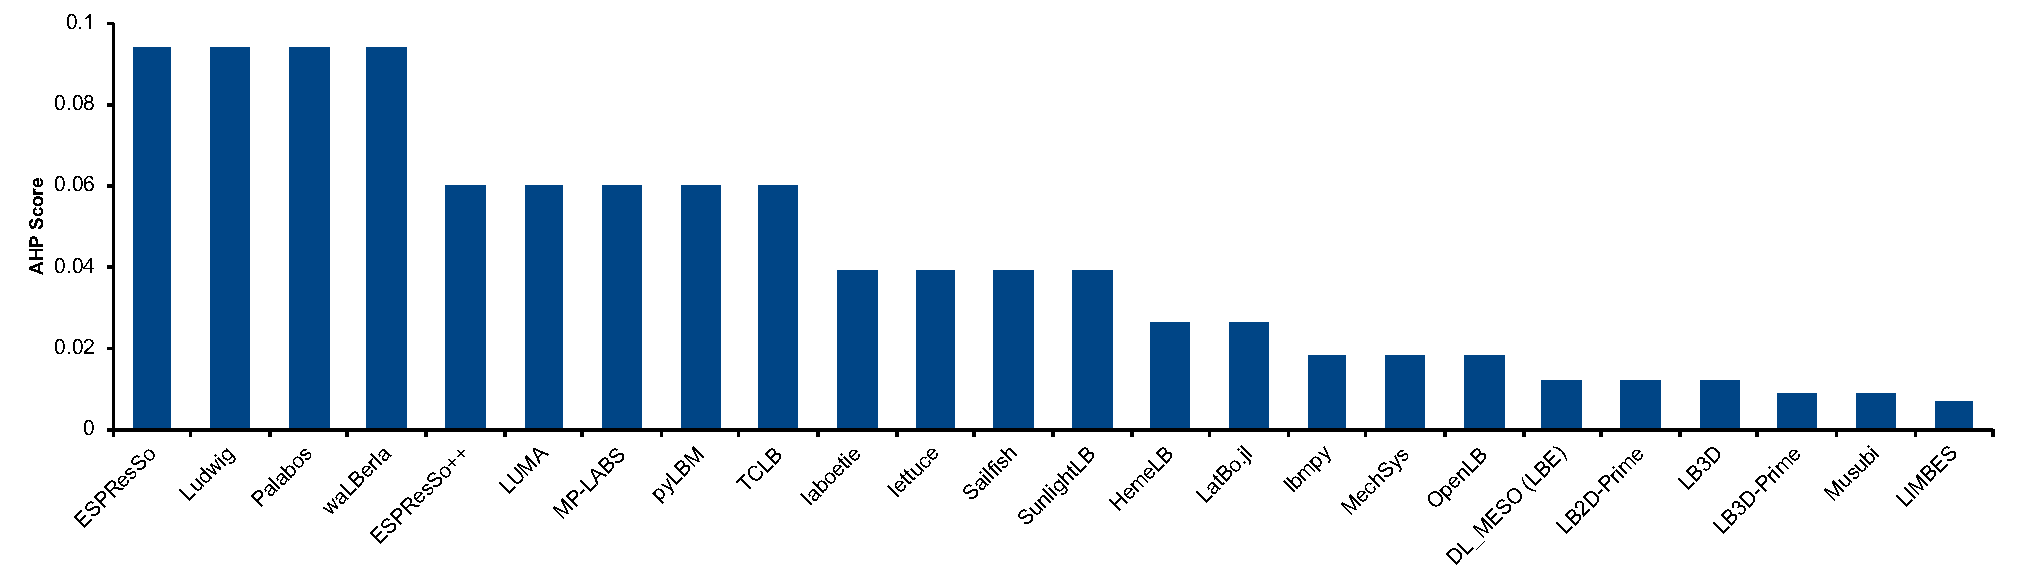
\includegraphics[width=1.0\textwidth]{./figures/maintainability_chart.pdf}
		\caption{AHP Maintainability Score}
		\label{Fig_Maintainability}
	\end{center}
\end{figure}

Figure~\ref{Fig_Maintainability} shows the maintainability ranking of the
software packages. Software packages with a high score provide version numbers
on documents and source code releases, have an abundance of high quality
artifacts, and use an issue tracking tool and version control system. These
packages also appear to manage their issue tracking, having most of their issues
closed. Maintainable packages by our ranking have more than 10\% of the code as
comments. \DIFdelbegin \DIFdel{Four }\DIFdelend \DIFaddbegin \DIFadd{All }\DIFaddend of the top \DIFdelbegin \DIFdel{five }\DIFdelend \DIFaddbegin \DIFadd{four }\DIFaddend ranked packages are alive.

\subsection{Reusability} \label{reusabilityresults}

We measure the total number of source code files for each project. We assume
that numerous source files increases reusability, since more files implies
increased modularization. Some packages have more features than others.  We
assume this contributes to reusability, since they have more source code for
potential reuse. We reviewed the software packages for the presence of API
documentation, which suggests that the developers considered potential future
reuse. 

\begin{figure}[h!]
	\begin{center}
		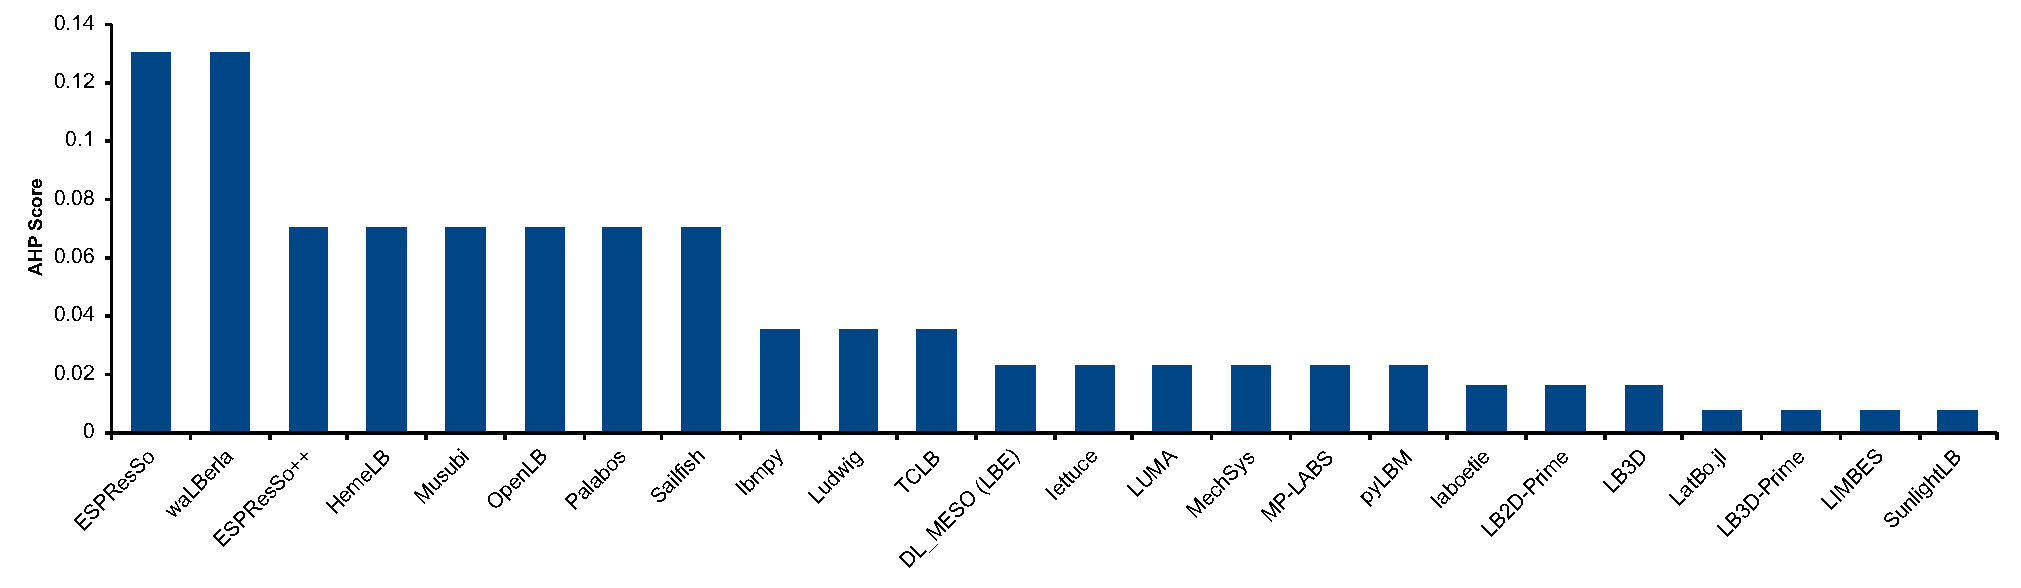
\includegraphics[width=1.0\textwidth]{./figures/reusability_chart.pdf}
		\caption{AHP Reusability Score}
		\label{Fig_Reusabilty}
	\end{center}
\end{figure}

Figure~\ref{Fig_Reusabilty} shows the reusability ranking of the software
packages. Software packages with a high score have thousands of source code
files and API documentation. The highest scoring packages, ESPResSo and
waLBerla, have extensive functionality, including graphical visualizations and
non-LBM modelling. For this reason, a comparison with other software packages is
not on a level field. \DIFdelbegin \DIFdel{Nine }\DIFdelend \DIFaddbegin \DIFadd{Seven }\DIFaddend of the top \DIFdelbegin \DIFdel{10 }\DIFdelend \DIFaddbegin \DIFadd{8 }\DIFaddend ranked packages are alive.

\begin{table}[ht!]
	\begin{center}
		\begin{tabular}{ p{3cm}p{2cm}p{2cm}p{2cm}p{3cm} }
			\toprule
			Name & Binary Files & LOC & Text Files & Avg.\ LOC / Text File \\
			\midrule
			LUMA & 19 & 4399723 & 314 & 14011 \\
			LatBo.jl & 0 & 42172 & 41& 1029 \\
			LB2D-Prime & 19 & 54755 & 82& 668 \\
			LB3D-Prime & 6 & 12944 & 23& 563 \\
			DL\_MESO (LBE) & 51 & 170223 & 310 & 549 \\
			LB3D & 76 & 39766 & 99 & 402 \\
			laboetie & 1 & 48403 & 133& 364 \\
			waLBerla & 69 & 873988 & 2643 & 331 \\
			MechSys & 3 & 95707 & 333 & 287 \\
			Palabos & 71 & 563841 & 1974 & 286 \\
			lbmpy & 29 & 61632 & 250 & 247 \\
			SunlightLB & 1 & 7646 & 36 & 212 \\
			Musubi & 1839 & 281879 & 1347 & 209 \\
			LIMBES & 1 & 4872 & 26 & 187 \\
			Ludwig & 32 & 162518 & 954 & 170 \\
			OpenLB & 7 & 218406 & 1438 & 152 \\
			ESPResSo & 83 & 195083 & 1390& 140 \\
			MP-LABS & 3 & 43124 & 307 & 140 \\
			pyLBM & 108 & 37234 & 272 & 137 \\
			\esp & 30 & 165194 & 1406& 118 \\
			HemeLB & 44 & 123806 & 1102& 112 \\
			Sailfish & 11 & 69398 & 632 & 110 \\
			lettuce & 1 & 7660 & 73 & 105 \\
			TCLB & 7 & 49156 & 594 & 83 \\
			\bottomrule
		\end{tabular}
		\caption{Module Data (Sorted by Avg.\ LOC / Text File)} \label{moduledata}
	\end{center}
\end{table}

Table~\ref{moduledata} shows file and Lines Of Code (LOC) data for the software
packages. Packages with a high reusability score do not have as many LOC per
text file, generally having a few hundred lines or fewer. We assume that
relatively small files implies modularization.

The package waLBerla scored high on reusability because of its focus on
modularity.  The modularity in the waLBerla framework enhances productivity,
reusability, and maintainability \citep{bauer2021walberla}. The design of
waLBerla has enabled it to be successfully applied as a basis for extension in
several projects \citep{bauer2021walberla}.

\subsection{Surface Understandability} \label{Sec_SurfUnderstandability}

To measure understandability, we review 10 random source code files per package.
Using only 10 files may incorrectly estimate understandability, but for
practical considerations we have to limit our time measuring each package.

All the packages appear to have consistent indentation and formatting. Only
HemeLB, LUMA, and Musubi explicitly identify coding standards that are used
during development. Generally, the software packages use consistent,
distinctive, and meaningful code identifiers. Only four packages (LB2D-Prime,
LB3D-Prime, LIMBES, MP-LABS) appear to use vague identifiers, such as single
letters for variables. Thirteen source code files use symbolic constants for
various parameters, mathematical constants, and matrix definitions. The code
includes appropriate comments for all packages, with the comments clearly
indicating what is being done (as opposed to how it is being done). The source
code of 11 packages include notes on domain algorithms. Table~\ref{moduledata}
suggests that the software packages are modular to various degrees. When
observing the source code files, 14 of the packages have a consistent style and
order of function parameters.

\begin{figure}[h!]
	\begin{center}
		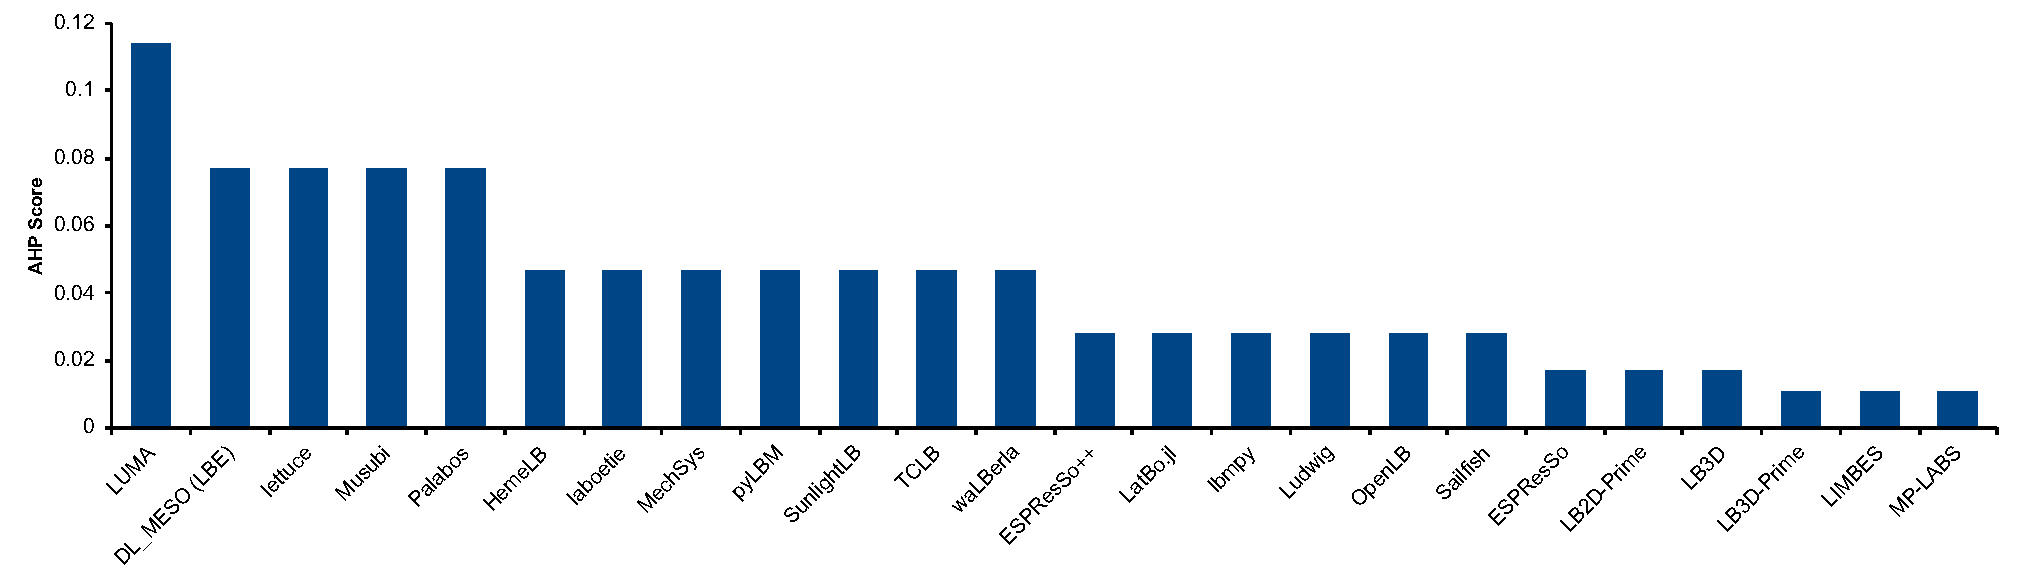
\includegraphics[width=1.0\textwidth]{./figures/understandability_chart.pdf}
		\caption{AHP Understandability Score}
		\label{Fig_Understandability}
	\end{center}
\end{figure}

Figure~\ref{Fig_Understandability} shows the surface understandability ranking.
Software packages with a high score have a consistent indentation and formatting
style, and consistent, distinctive, and meaningful code identifiers. They also
have symbolic constants, and explicitly identify mathematical and LBM
algorithms. Their comments are clear and indicate what is being done in the
source code. The source code is well modularized and structured. All the top
five ranked packages are alive.

\subsection{Visibility and Transparency}

We review the software artifacts for process documentation, a development
environment description, and release notes.  The packages tend to not explicitly
use well-known development models (see also
Section~\ref{Sec_CompareMethodologies}). The development teams of these packages
are fairly small and easily organized without the need for such processes. Seven
of the software packages did have some artifacts outlining the general
development process, how to contribute, and the status of the package or its
components. Eight of the packages have artifacts that note the development
environment. While this information could help developers, and would improve
transparency, the small close-knit nature of the development teams make
explicitly specifying this information practically unnecessary. Nine of the
software packages included version release notes.

\begin{figure}[h!]
	\begin{center}
		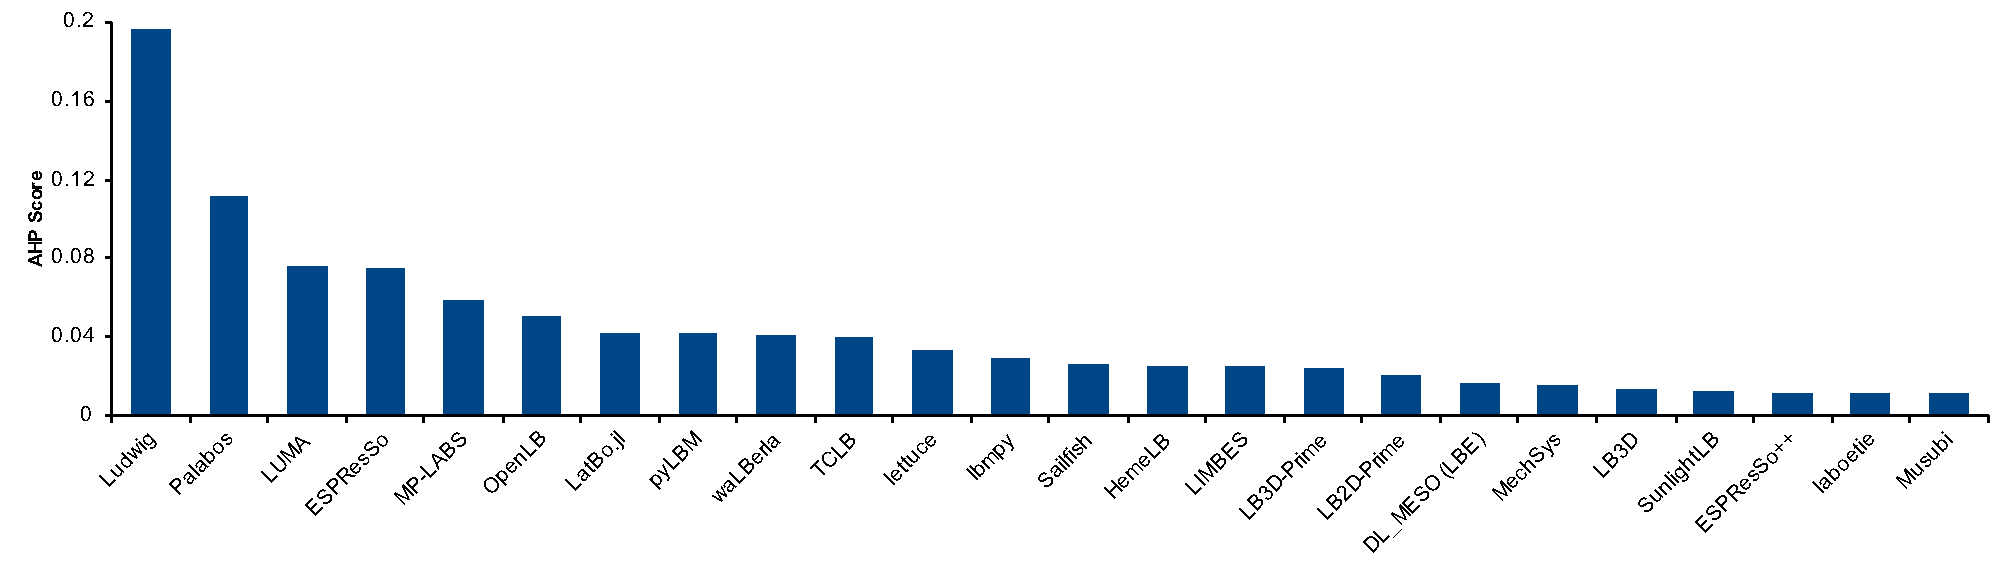
\includegraphics[width=1.0\textwidth]{./figures/visibilitytransparency_chart.pdf}
		\caption{AHP Visibility and Transparency Score}
		\label{Fig_VisibilityTransparency}
	\end{center}
\end{figure}

Figure~\ref{Fig_VisibilityTransparency} shows the visibility and transparency
ranking of the software packages. Software packages with a high score have an
explicit development model and defined development process. They also have
detailed and easy to access software release notes. \DIFdelbegin \DIFdel{Four of }\DIFdelend \DIFaddbegin \DIFadd{All }\DIFaddend the top five ranked
packages are alive.

\subsection{Overall Quality} \label{Sec_OverallQuality}

\begin{figure}[h!]
	\centering
		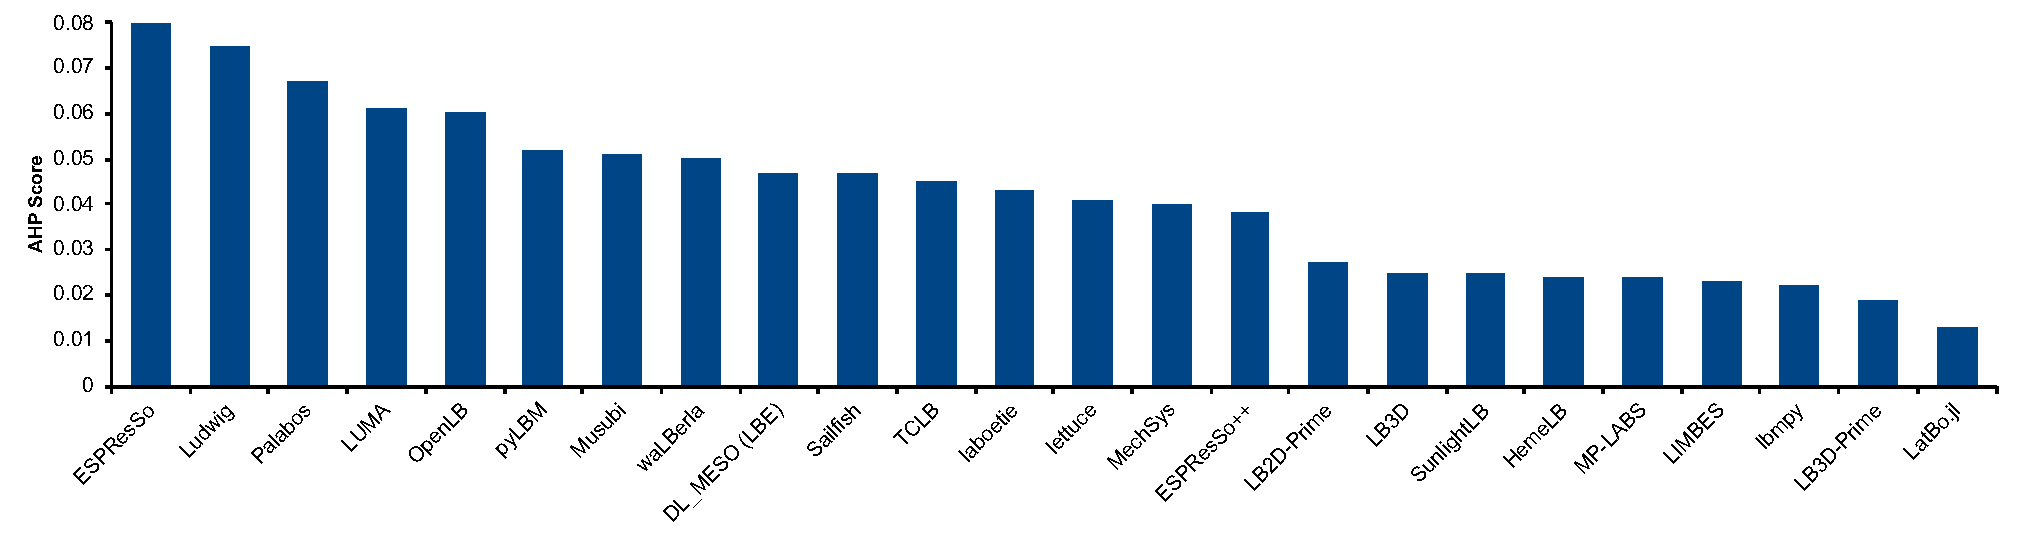
\includegraphics[width=1.0\textwidth]{./figures/finalscore_chart.pdf}
		\caption{AHP Overall Score}
		\label{Fig_OverallScore}
\end{figure}

Figure~\ref{Fig_OverallScore} shows the overall ranking. \DIFaddbegin \DIFadd{The AHP method finds
the weighting of quality $i$ ($w_i$) in the same way that the score ($s_j$) was
found for software package $j$ evaluated for a given quality
(Section~\ref{AHP}).  That is, we conduct a pairwise comparison between the
priority of different qualities to construct the $m \times m$ matrices $A$ and
$B$, and then we average row $i$ of matrix $B$ to find the priority value $w_i$
for quality $i$.  If we introduce the notation that $s^i_j$ is the score for
quality $i$ for package $j$, then the overall score $S_j$ for package $j$ is
found via:
}

$$\DIFadd{S_j = \sum_{i=1}^m s^i_j w_i}$$

\DIFaddend In the absence of other information on priorities, we calculated the ranking by
assuming an equal weighting between all qualities. Software packages with an
overall high score ranked high in at least several of the individual qualities.

Looking at the top three ranked packages: ESPResSo achieved a relatively high
score in installability, surface usability, maintainability, reusability, and
visibility and transparency. Ludwig scored high in surface correctness and
verifiability, surface robustness, surface usability, maintainability, and
visibility and transparency. Palabos scored high in installability, surface
reliability, surface robustness, maintainability, understandability, and
visibility and transparency.

\section{Comparison to Community Ranking} \label{repmetrics}

To address \rqref{RQ_CompareHQ2Popular}, Table~\ref{repometrics} compares our
LBM software rankings against their popularity in the research community, as
estimated by repository stars and watches. Nine packages do not use GitHub, so
they do not have a measure of repository stars. Looking at the repository stars
of the other 15 packages, we observe a pattern where packages that have been
highly ranked by our assessment tend to have more stars than lower ranked
packages. Our best ranked package (ESPResSo) has the second most stars, while
our ninth ranked package (Sailfish) has the highest number of stars. The
repository watch column shows the same correlation, although this column
contains less data, since two of the packages (Palabos, waLBerla) use GitLab,
which does not track watches. Consistent with the star measure, our ninth ranked
package (Sailfish) has the highest number of watches and our best ranked package
(ESPResSo) has the second most watches. Packages designated as lower quality
often do not use GitHub or GitLab, or have only a few stars and watches.
Although the details of the rankings differ, our measures show that following
best practices tends to correlate with increased popularity in the scientific
community.

Notable exceptions to this trend occur for three projects that rank high by star
count, but relatively low in the ``follow best practices'' ranking: TCLB (star
rank 3, our rank \DIFdelbegin \DIFdel{12}\DIFdelend \DIFaddbegin \DIFadd{10}\DIFaddend ), lettuce (star rank 4, our rank \DIFdelbegin \DIFdel{14}\DIFdelend \DIFaddbegin \DIFadd{12}\DIFaddend ) and \esp{} (star rank
5, our rank \DIFdelbegin \DIFdel{15}\DIFdelend \DIFaddbegin \DIFadd{14}\DIFaddend ).  Part of the discrepancy is because our process ranks all
projects, but the star measure does not apply to all projects.  Also, our
process equally weights all qualities (Section~\ref{Sec_OverallQuality}), but
for real users some qualities will be more important than others. Discrepancies
between our measures and the star measures may also be due to inaccuracy with
using stars to approximate popularity, because of how people use stars, because
young projects have less time to accumulate stars, and because stars represent
the community's feeling in the past more than current preferences
\citep{Szulik2017}. Older packages (like \esp{} and TCLB) have had more time to
accumulate stars and watches. Young projects have less time to accumulate stars,
like HemeLB, which only has 12 stars (at the time of measurement) having
recently moved from a different GitHub repository.  Lettuce is a young project
(released in 2019) with a relatively high number of stars. The discrepancy in
rankings may be due to a mismatch between the time we manually measured lettuce
and when we counted the stars. The late addition of Musubi means a gap between
when we measured projects and the time when our automated data (like stars) was
collected. A final reason for inconsistencies between our ranking and the
community's ranking is that, as for consumer products, more factors influence
popularity than just quality.

\begin{table}[ht!]
	\begin{center}
		\begin{tabular}{ p{3cm}p{1.25cm}p{1.75cm}p{1.75cm}p{1.75cm}p{1.75cm} }
			\toprule
			Name & Our Ranking & Repository Stars & Repository Star Rank &
			Repository Watches & Repository Watch Rank\\
			\midrule
			ESPResSo & 1 & 145 & 2 & 19& 2\\
			Ludwig & 2 & 27 & 8 & 6 & 7\\
			Palabos & 3 & 34 & 6 & GitLab & GitLab\\
			\DIFdelbeginFL \DIFdelFL{OpenLB }\DIFdelendFL \DIFaddbeginFL \DIFaddFL{LUMA }\DIFaddendFL & 4 & \DIFaddbeginFL \DIFaddFL{33 }& \DIFaddFL{7 }& \DIFaddFL{12 }& \DIFaddFL{4}\\
			\DIFaddFL{OpenLB }& \DIFaddFL{5 }& \DIFaddendFL N/A & N/A & N/A& N/A\\
			\DIFdelbeginFL \DIFdelFL{LUMA }%DIFDELCMD < & %%%
\DIFdelFL{5 }%DIFDELCMD < & %%%
\DIFdelFL{33 }%DIFDELCMD < & %%%
\DIFdelFL{7 }%DIFDELCMD < & %%%
\DIFdelFL{12 }%DIFDELCMD < & %%%
\DIFdelFL{4}%DIFDELCMD < \\
%DIFDELCMD < 			%%%
\DIFdelendFL pyLBM & 6 & 95 & 3 & 10 & 5\\
			\DIFdelbeginFL \DIFdelFL{DL\_MESO (LBE) }\DIFdelendFL \DIFaddbeginFL \DIFaddFL{Musubi }\DIFaddendFL & 7 & N/A & N/A & N/A & N/A\\
			\DIFdelbeginFL \DIFdelFL{Musubi }\DIFdelendFL \DIFaddbeginFL \DIFaddFL{waLBerla }\DIFaddendFL & 8 & \DIFaddbeginFL \DIFaddFL{20 }& \DIFaddFL{9 }& \DIFaddFL{GitLab }& \DIFaddFL{GitLab}\\
			\DIFaddFL{DL\_MESO (LBE) }& \DIFaddFL{9 }& \DIFaddendFL N/A & N/A & N/A & N/A\\
			Sailfish & 9 & 186 & 1 & 41& 1\\
			\DIFdelbeginFL \DIFdelFL{waLBerla }\DIFdelendFL \DIFaddbeginFL \DIFaddFL{TCLB }\DIFaddendFL & 10 & \DIFdelbeginFL \DIFdelFL{20 }\DIFdelendFL \DIFaddbeginFL \DIFaddFL{95 }\DIFaddendFL & \DIFdelbeginFL \DIFdelFL{9 }\DIFdelendFL \DIFaddbeginFL \DIFaddFL{3 }\DIFaddendFL & \DIFdelbeginFL \DIFdelFL{GitLab }\DIFdelendFL \DIFaddbeginFL \DIFaddFL{16 }\DIFaddendFL & \DIFdelbeginFL \DIFdelFL{GitLab}\DIFdelendFL \DIFaddbeginFL \DIFaddFL{3}\DIFaddendFL \\
			laboetie & 11 & 4 & 13 & 5 & 8\\
			\DIFdelbeginFL \DIFdelFL{TCLB }\DIFdelendFL \DIFaddbeginFL \DIFaddFL{lettuce }\DIFaddendFL & 12 & \DIFdelbeginFL \DIFdelFL{95 }\DIFdelendFL \DIFaddbeginFL \DIFaddFL{48 }\DIFaddendFL & \DIFdelbeginFL \DIFdelFL{3 }\DIFdelendFL \DIFaddbeginFL \DIFaddFL{4 }\DIFaddendFL & \DIFdelbeginFL \DIFdelFL{16 }\DIFdelendFL \DIFaddbeginFL \DIFaddFL{5 }\DIFaddendFL & \DIFdelbeginFL \DIFdelFL{3}\DIFdelendFL \DIFaddbeginFL \DIFaddFL{8}\DIFaddendFL \\
			MechSys & 13 & N/A & N/A & N/A & N/A\\
			\DIFdelbeginFL \DIFdelFL{lettuce }\DIFdelendFL \DIFaddbeginFL \esp \DIFaddendFL & 14 & \DIFdelbeginFL \DIFdelFL{48 }%DIFDELCMD < & %%%
\DIFdelFL{4 }%DIFDELCMD < & %%%
\DIFdelFL{5 }%DIFDELCMD < & %%%
\DIFdelFL{8}%DIFDELCMD < \\
%DIFDELCMD < 			\esp & %%%
\DIFdelFL{15 }%DIFDELCMD < & %%%
\DIFdelendFL 35 & 5 & 12 & 4\\
			\DIFdelbeginFL \DIFdelFL{MP-LABS }\DIFdelendFL \DIFaddbeginFL \DIFaddFL{LB2D-Prime }\DIFaddendFL & \DIFdelbeginFL \DIFdelFL{16 }\DIFdelendFL \DIFaddbeginFL \DIFaddFL{15 }\DIFaddendFL & \DIFdelbeginFL \DIFdelFL{12 }%DIFDELCMD < & %%%
\DIFdelFL{11 }%DIFDELCMD < & %%%
\DIFdelFL{2 }%DIFDELCMD < & %%%
\DIFdelFL{9}%DIFDELCMD < \\			
%DIFDELCMD < 			%%%
\DIFdelFL{SunlightLB }%DIFDELCMD < & %%%
\DIFdelFL{17 }%DIFDELCMD < & %%%
\DIFdelendFL N/A & N/A & N/A & N/A\\
			LB3D & \DIFdelbeginFL \DIFdelFL{18 }\DIFdelendFL \DIFaddbeginFL \DIFaddFL{16 }\DIFaddendFL & N/A & N/A & N/A & N/A\\
			\DIFdelbeginFL \DIFdelFL{LIMBES }\DIFdelendFL \DIFaddbeginFL \DIFaddFL{SunlightLB }\DIFaddendFL & \DIFdelbeginFL \DIFdelFL{19 }\DIFdelendFL \DIFaddbeginFL \DIFaddFL{16 }\DIFaddendFL & N/A & N/A & N/A & N/A\\
			\DIFdelbeginFL \DIFdelFL{LB2D-Prime }\DIFdelendFL \DIFaddbeginFL \DIFaddFL{HemeLB }\DIFaddendFL & \DIFdelbeginFL \DIFdelFL{20 }\DIFdelendFL \DIFaddbeginFL \DIFaddFL{17 }\DIFaddendFL & \DIFaddbeginFL \DIFaddFL{12 }& \DIFaddFL{11 }& \DIFaddFL{12 }& \DIFaddFL{4}\\
			\DIFaddFL{MP-LABS }& \DIFaddFL{17 }& \DIFaddFL{12 }& \DIFaddFL{11 }& \DIFaddFL{2 }& \DIFaddFL{9}\\
			\DIFaddFL{LIMBES }& \DIFaddFL{18 }& \DIFaddendFL N/A & N/A & N/A & N/A\\
			\DIFdelbeginFL \DIFdelFL{HemeLB }%DIFDELCMD < & %%%
\DIFdelFL{21 }%DIFDELCMD < & %%%
\DIFdelFL{12 }%DIFDELCMD < & %%%
\DIFdelFL{11 }%DIFDELCMD < & %%%
\DIFdelFL{12 }%DIFDELCMD < & %%%
\DIFdelFL{4}%DIFDELCMD < \\
%DIFDELCMD < 			%%%
\DIFdelendFL lbmpy & \DIFdelbeginFL \DIFdelFL{22 }\DIFdelendFL \DIFaddbeginFL \DIFaddFL{19 }\DIFaddendFL &  11 & 12 & 2 & 9\\
			LB3D-Prime & \DIFdelbeginFL \DIFdelFL{23 }\DIFdelendFL \DIFaddbeginFL \DIFaddFL{20 }\DIFaddendFL & N/A & N/A & N/A & N/A\\
			LatBo.jl & \DIFdelbeginFL \DIFdelFL{24 }\DIFdelendFL \DIFaddbeginFL \DIFaddFL{21 }\DIFaddendFL & 17 & 10 & 8 & 6\\
			\bottomrule
		\end{tabular}
		\caption{Repository Ranking Metrics (Sorted by Our Ranking)} \label{repometrics}
	\end{center}
\end{table}

Although our ranking and the estimate of the community's ranking are not perfect
measures, they do suggest a correlation between best practices and popularity.
We do not know which comes first, the use of best practices or popularity, but
we do know that the top ranked packages tend to incorporate best practices.  The
next sections will explore how the practices of the LBM community compare to the
broader research software community.  We will also investigate the practices
from the top projects that others within the LBM community and beyond can
potentially adopt.

\section{Comparison Between LBM and Other Research Software for Artifacts}
\label{Sec_CompareArtifacts}

As part of filling in the measurement template, we listed the artifacts for each
package, and then categorized them by frequency. We group the artifacts into
common, uncommon, and rare categories in Table~\ref{artifactspresent}. Common
artifacts are in 16 to 24 ($>$63\%) of the software packages. Uncommon artifacts
are in 8 to 15 (30-63\%) and rare artifacts are in 1 to 7 ($<$30\%) of the
packages.  We answer \rqref{RQ_CompareArtifacts} by comparing the artifacts that
we observed in LBM repositories to those observed and recommended for research
software in general.

\begin{table}[ht!]
\begin{center}
\begin{tabular}{ p{5.3 cm} p{4.9 cm} p{5 cm}}
\toprule
\textbf{Common} & \textbf{Uncommon} & \textbf{Rare} \\
\midrule
Authors / Developers List & Change Log / Release Notes & Acknowledgements\\
Getting Started & Citation & API Documentation\\
Installation Guide / Instructions & Contributing & Code Style Guide\\
Issue Tracker & Design Documentation & Developer / Contributor Manual\\
Library Dependency List & Functional Spec. / Notes & FAQ / Forum\\
License & Performance Information & Requirements Spec.\\
List of Related Publications & Test Plan / Script / Cases & Product Roadmap\\
Makefile / Build File & User Manual / Guide & Uninstall\\
README File & & Verification and Validation Plan\\
Theory Notes & & Video Guide (including YouTube)\\
Tutorial & & \\
Version Control & & \\
\bottomrule
\end{tabular}
\caption{Artifacts Present in LBM Packages, Classified by Frequency (Sorted Alphabetically)}
\label{artifactspresent}
\end{center}
\end{table}

Table~\ref{Tbl_Guidelines} (based on data from \citep{SmithAndMichalski2022}) %DOUBLE BLIND
shows that LBM artifacts generally match the recommendations found in nine
current research software development guidelines:
\begin{itemize}
\item United States Geological Survey Software Planning Checklist
\citep{USGS2019},
\item DLR (German Aerospace Centre) Software Engineering Guidelines
\citep{TobiasEtAl2018}, 
\item Scottish Covid-19 Response Consortium Software Checklist
\citep{BrettEtAl2021},
\item Good Enough Practices in Scientific Computing \citep{WilsonEtAl2016},
\item xSDK (Extreme-scale Scientific Software Development Kit) Community Package
Policies \citep{SmithAndRoscoe2018},
\item Trilinos Developers Guide \citep{HerouxEtAl2008},
\item EURISE (European Research Infrastructure Software Engineers') Network
Technical Reference \citep{ThielEtAl2020},
\item CLARIAH (Common Lab Research Infrastructure for the Arts and Humanities)
Guidelines for Software Quality \citep{vanGompelEtAl2016}, and
\item A Set of Common Software Quality Assurance Baseline Criteria for Research
Projects \citep{OrvizEtAl2017}.
\end{itemize}

In Table~\ref{Tbl_Guidelines}, each row corresponds to an artifact.  For a given
row, a checkmark in one of the columns means that the corresponding guideline
recommends this artifact.  The last column shows whether the artifact appears in
the measured set of LBM software, either not at all (blank), commonly (C),
uncommonly (U) or rarely (R).  We did our best to interpret the meaning of each
artifact consistently between guidelines and specific MI software, but the
terminology and the contents of artifacts are not standardized.  This challenge
even exists for the ubiquitous README file.  As illustrated by
\citet{PranaEtAl2018}, the content of README files shows significant variation
between projects.  Although some content is reasonably consistent, with 97\% of
README files containing at least one section describing the `What` of the
repository and 88.5 \% offering some `How` content, other categories are more
variable.  For instance, information on `Contribution`, `Why`, and `Who`,
appear in 27.8\%, 25.7\% and 52.9\% of the analyzed files, respectively
\citep{PranaEtAl2018}.  

The frequency of checkmarks in Table~\ref{Tbl_Guidelines} indicates the
popularity of recommending a given artifact, but it does not imply that the most
commonly recommended artifacts are the most important artifacts. Moreover, just
because a guideline does not explicitly recommend an artifact does not mean that
the artifact has no value.  The guideline authors may have excluded it because
it is out of the scope of their recommendations or outside their experience. For
instance, an artifact related to uninstall is only explicitly mentioned by
\citet{vanGompelEtAl2016}, but other guideline authors would likely see its
value.  They may simply feel that uninstall is implied by install, or they may
have never asked themselves about the need for separate uninstall instructions.

\begin{table}[!ht]
\begin{center}
\begin{tabular}{ p{2.5cm}p{1cm}p{1cm}p{1cm}p{1cm}p{1cm}p{1cm}p{1cm}p{1.2cm}p{1cm}p{0.8cm} }
\toprule
~ \ & \citet{USGS2019} & \citet{TobiasEtAl2018} & \citet{BrettEtAl2021} &
\citet{WilsonEtAl2016} & \citet{SmithAndRoscoe2018} & \citet{HerouxEtAl2008} &
\citet{ThielEtAl2020} & \citet{vanGompelEtAl2016} & \citet{OrvizEtAl2017} &
LBM\\
\midrule
LICENSE & \checkmark & \checkmark & \checkmark & \checkmark & \checkmark & & \checkmark & \checkmark & \checkmark & C\\
README &  & \checkmark & \checkmark & \checkmark & \checkmark & & \checkmark & \checkmark & \checkmark & C\\
CONTRIBUTING &  & \checkmark & \checkmark & \checkmark & \checkmark & & \checkmark & \checkmark & \checkmark & U\\
CITATION &  &  &  & \checkmark & & & & \checkmark & \checkmark & U\\
CHANGELOG &  & \checkmark &  & \checkmark & \checkmark & & \checkmark &  &  & U\\
INSTALL &  &  &  &  & \checkmark & & \checkmark & \checkmark & \checkmark & C\\
\midrule
Uninstall &  &  &  &  & & & & \checkmark & & R\\
Dependency List &  &  & \checkmark & & \checkmark & & & \checkmark &  & C\\
Authors &  &  &  &  &  &  & \checkmark & \checkmark & \checkmark & C\\
Code of Conduct &  &  &  &  & & & \checkmark & & & \\
Acknowledgements &  &  &  &  &  &  & \checkmark & \checkmark & \checkmark & R\\
Code Style Guide &  & \checkmark &  &  & & & \checkmark & \checkmark & \checkmark & R\\
Release Info. &  & \checkmark &  &  & & \checkmark & \checkmark & & & U\\
Prod.\ Roadmap &  &  &  &  & & \checkmark & \checkmark & \checkmark & & R\\
\midrule
Getting started &  &  &  &  & \checkmark & & \checkmark & \checkmark & \checkmark & C\\
User manual &  &  & \checkmark &  & & & \checkmark & & & U\\
Tutorials &  &  &  &  & & & \checkmark & & & C\\
FAQ &  &  &  &  & & & \checkmark & \checkmark & \checkmark & R\\
\midrule
Issue Track &  & \checkmark & \checkmark & & \checkmark & \checkmark & \checkmark & & \checkmark & C\\
Version Control &  & \checkmark & \checkmark & \checkmark & \checkmark & \checkmark & \checkmark & \checkmark & \checkmark & C\\ 
Build Scripts &  & \checkmark &  & \checkmark & \checkmark & \checkmark &
\checkmark & & \checkmark & C\\
\midrule
Requirements &  & \checkmark &  &  & & \checkmark &  &  & \checkmark &  \\
Design Doc.\ &  & \checkmark  & \checkmark &  & \checkmark & & \checkmark &
\checkmark& \checkmark & U\\
API Doc. &  &  &  &  & \checkmark & & \checkmark & \checkmark & \checkmark & R\\
Test Plan &  & \checkmark &  &  & & \checkmark & & & &  U\\
Test Cases & \checkmark & \checkmark & \checkmark &  & \checkmark & \checkmark &
\checkmark & \checkmark & \checkmark & U\\
\bottomrule
\end{tabular}
\caption{Comparison of Recommended Artifacts in Software Development Guidelines
to Artifacts in LBM Projects (C for Common, U for Uncommon and R for Rare)}
\label{Tbl_Guidelines}
\end{center}
\end{table}

The top \DIFdelbegin \DIFdel{four }\DIFdelend \DIFaddbegin \DIFadd{three }\DIFaddend packages (ESPREsSo, Ludwig, Palabos\DIFdelbegin \DIFdel{, and OpenLB}\DIFdelend ) include most of
the common and uncommon artifacts, but not many of the rare artifacts.  They
collectively have all the common artifacts, except Palabos does not have theory
notes\DIFdelbegin \DIFdel{, and OpenLB does not appear to use version control}\DIFdelend .  The top \DIFdelbegin \DIFdel{four }\DIFdelend \DIFaddbegin \DIFadd{three }\DIFaddend packages
have most of the uncommon artifacts. Only one them (Ludwig) is missing design
information, and only one (Palabos) does not have a user manual.  However, for
Palabos there was a broken link on the package website indicating that such an
artifact might exist. The developers later fixed this broken link, but this is
not reflected in our data because it was not present at the time of data
collection (mid-2020). Despite the broken link, Palabos does have a detailed and informative website. The top \DIFdelbegin \DIFdel{four }\DIFdelend \DIFaddbegin \DIFadd{three }\DIFaddend ranked packages do not have many of the rare artifacts. None of them have any explicit API documentation. \DIFdelbegin \DIFdel{Three of them (ESPREsSo, Ludwig, Palabos) }\DIFdelend \DIFaddbegin \DIFadd{All of them }\DIFaddend have information on contributing to the project and
\DIFdelbegin \DIFdel{two (OpenLB, Palabos) have }\DIFdelend \DIFaddbegin \DIFadd{one (Palabos) has }\DIFaddend an FAQ section or forum. 
\DIFdelbegin \DIFdel{One (OpenLB) has
verification and validation notes, and a video guide for the software. 
}\DIFdelend 

Three of the items that appear in Table~\ref{artifactspresent} do not explicitly
appear in the software development guidelines: i) list of related publications,
ii) performance information and iii) video guides.  The occurrence of the first
two items in this list are likely more a consequence of how we collected our
list of LBM artifacts, rather than being a unique practice of LBM developers. We
highlighted publications and performance information because we were explicitly
looking for both as part of our measurement template. Related
publications and performance information certainly appear in other research
software projects; the practices just are not highlighted in guidelines because
they are implicit in other documentation recommendations, such as theory
documentation and user guides. The observation of a video guide artifact is more
novel.  \citet{Fogel2005} recommends videos for open source projects, and other
projects likely use them, but the practice has apparently not yet made it into
research software community's guidelines.  Putting aside the debate of the
effectiveness of learning from print versus video, video documentation is
growing in popularity, with a majority of Generation Z learners preferring video
to print \citep{Genota2018}.

As Table~\ref{Tbl_Guidelines} shows, the LBM community participates in most
practices we found listed in the general research software guidelines; however,
we did not observe, or rarely observed, some recommended practices. For
instance, we rarely saw API documentation for LBM software, but it is a
frequently recommended artifact \citep{SmithAndRoscoe2018, ThielEtAl2020,
vanGompelEtAl2016, OrvizEtAl2017, SSI2022, Zadka2018}.  In addition to the items
in the last column of Table~\ref{artifactspresent}, we can add the following
community recommended items that we rarely, if ever, observed:

\begin{itemize}

\item \textbf{A roadmap} is considered by some to be a critical document for an
organization to map out the vision and direction for a product offering
\citep{MunchEtAl2019}.  Roadmaps take different forms, but they all aim to
address the following: \begin{inparaenum}[i)]
	\item Where are we now?,
	\item Where are we going?, and
	\item How can we get there? \end{inparaenum} \citep{PhaalEtAl2005}.
Developers can create a roadmap by the following steps:
\begin{inparaenum}[i)]
	\item define and outline a strategic mission and product vision, 
	\item scan the environment, 
	\item revise and distill the product vision to write the product roadmap, and 
	\item estimate the product life cycle and evaluate the mix of planned
development efforts \end{inparaenum} \citep{VahaniittyEtAl2002}.  A product
roadmap has the benefits of providing continuity of purpose, facilitating
stakeholder collaboration and assisting with prioritization \citep{Pichler2012}.
Although we saw some elements of a roadmap in the LBM projects, we did not
observe a specific artifact devoted to this purpose.

\item \textbf{A code of conduct} documents expectations and standards of ethical
behaviour and explicitly states how developers should treat one another
\citep{TouraniEtAl2017}. A code of conduct outlines rules for communication,
establishes enforcement mechanisms for violations and codifies the spirit of a
community, such that anyone can contribute comfortably regardless of, for
example, ethnicity, gender, or sexual orientation \citep{TouraniEtAl2017}. The
top three most popular code's of conduct from \citet{TouraniEtAl2017} are:
\href{https://ubuntu.com/community/code-of-conduct} {Ubuntu Code of Conduct},
\href{https://www.contributor-covenant.org/version/2/1/code_of_conduct/}
{Contributor Covenant}, and \href{https://www.djangoproject.com/conduct/}
{Django Code of Conduct}. \citet{SinghEtAl2021} shows the value of adopting a
code of conduct on the participation of women. Improved inclusivity means a
wider pool of potential contributors. Moreover, a code of conduct facilitates
meeting ethical obligations for developers that abide by a code of ethics, such
as the IEEE Code of Ethics \citep{IEEE1999}, or the Professional Engineers of
Ontario code of ethics \citep[p.\ 23--24]{PEO2021}. For the LBM software, we did
not observe any codes of conduct, possibly because the number of developers for
each project is small and because the idea has not yet occurred to them.

\item \textbf{Code style guides} provide rules and guidance on writing code.
Style guides standardize such elements as naming identifiers, formatting, code
comments, best practices and dangers to avoid \citep{Carty2020}. An example of a
ubiquitous coding standard is to use ALLCAPS for symbolic constants.
Standardization improves understandability (Section~\ref{softwarequalities}),
since developers spend more time on the content of the code, and less time
distracted by its style.  Three example style guides include:
\href{http://cnl.sogang.ac.kr/cnlab/lectures/programming/python/PEP8_Style_Guide.pdf}
{PEP8 Style Guide for Python},
\href{https://google.github.io/styleguide/javaguide.html} {Google Java Style
Guide} and \href{https://google.github.io/styleguide/cppguide.html} {Google \CC
Style Guide}.  Tools like \href{https://pypi.org/project/flake8/}{flake8} can be
used to automatically check that coding styles, in this case PEP8, are enforced.
For LBM software we saw code style advice as part of some developer guides, but
only rarely.

\item \textbf{Checklists} can be used to ensure that developers follow best
practices.  Some examples include checklists merging branches into master
\citep{Brown2015}, checklists for saving and sharing changes to the project
\citep{WilsonEtAl2016}, checklists for new and departing team members
\citep{HerouxAndBernholdt2018}, checklists for processes related to commits and
releases \citep{HerouxEtAl2008} and checklists for overall software quality
\citep{ThielEtAl2020, SSI2022}.  For LBM software, ESPResSo has a checklist for
managing releases, but we did not see any other examples.

\item \textbf{Uninstall instructions} tell a user how to remove the software and
associated libraries from their system.  Uninstall removes files that consume
space and potentially pollute the user's build system with potential future
compilation and linking conflicts.  Only one software package (pyLBM) has
uninstallation instructions.

\item \textbf{API documentation} shows programmers the services or data provided
by the software application (or library) through such resources as its methods
or objects \citep{MengEtAl2018}.  API documentation is a critical factor for API
understandability \citep{MengEtAl2018} (Section~\ref{softwarequalities}). Some
API documentation can be generated using tools like Doxygen, but when learning a
new API developers mostly use code examples and tutorials \citep{MengEtAl2018}.
API documentation is rare within our sample of LBM packages.

\end{itemize}

Where data is available, LBM software artifacts can be compared to other
research software domains.  Compared to ocean modelling software
\citep{JungEtAl2022}, LBM software seems to pay more attention to artifacts
related to testing.  Compared to Medical Imaging Software \citep{Dong2021}, the
artifact frequency is similar, except LBM software is more likely to have
developer related artifacts, like Contributing, Dependency list, and Design
documentation.

Table~\ref{Tbl_Guidelines} shows that many LBM projects fall short of
recommended best practices for research software.  However, LBM software is not
alone in this.  Many, if not most, research projects fall short of best
practices.  A gap exists in research software development practices and software
engineering recommendations \citep{Storer2017, Kelly2007, OwojaiyeEtAl2021_CSE}.
\citet{JohansonAndHasselbring2018} observe that the state-of-the-practice for
research software in industry and academia does not incorporate state-of-the-art
SE tools and methods.  This causes sustainability and reliability problems
\citep{FaulkEtAl2009}. Rather than benefit from capturing and reusing previous
knowledge, projects waste time and energy ``reinventing the wheel''
\citep{deSouzaEtAl2019}. 

Software requirements documentation provides a good example of the common
deviation between recommendations and practice.  Although some guidelines
recommend requirements documentation \citep{TobiasEtAl2018, HerouxEtAl2008,
SmithAndKoothoor2016}, in practice research software developers often do not
produce a proper requirements specification \citep{HeatonAndCarver2015}.
\citet{SandersAndKelly2008} interviewed 16 scientists from 10 disciplines and
found that none of the scientists created requirements specifications, unless
regulations in their field mandated such a document. \citet{Nguyen-HoanEtAl2010}
shows requirements are the least commonly produced type of documentation for
research software in general. When looking at the pain points for research
software developers, \citet{WieseEtAl2019} state that software requirements and
management is the software engineering discipline that most hurts scientific
developers, accounting for 23\% of the technical problems reported by study
participants.  The lack of support for requirements is likely due to the
perception that up-front requirements are impossible for research software
\citep{CarverEtAl2007, SegalAndMorris2008}, but when we drop the insistence on
``up-front'' requirements, allowing the requirements to be written
iteratively and incrementally, requirements are feasible \citep{Smith2016}.

\section{Comparison of Tool Usage Between LBM and Other Research Software}
\label{Sec_CompareTools}

Developers use software tools to support the development, verification,
maintenance, and evolution of software, software processes, and artifacts
\citep[p.\ 501]{GhezziEtAl2003}. Table~\ref{tbl_tools} summarizes the observed
tools, subdivided into development tools, dependencies, and project management
tools. In this section we answer \rqref{RQ_CompareToolsProjMngmnt} by comparing
aspects of tool usage in LBM software packages to their use in the research
software community in general.

\begin{table}[ht!]
	\begin{center}
	\begin{tabular}{ p{5.3 cm} p{4.9 cm} p{5 cm}}
	\toprule
	\textbf{Development Tools} & \textbf{Dependencies} & \textbf{Project
	Management Tools} \\
	\midrule
	Code Editors & Build Automation Tools & Change Tracking Tools\\
	Compilers & Domain Specific Libraries & Collaboration Tools\\
	Continuous Integration & Technical Libraries & Document Generation Tools\\
	Correctness Verification Tools &  & Email\\
	Development Environments &  & Version Control Tools\\
	Runtime Environments &  & \\
	Unit Testing Tools &  & \\
	\bottomrule
	\end{tabular}
	\caption{Observed development tools, dependencies and project management
	tools (Sorted Alphabetically)} \label{tbl_tools}
	\end{center}
\end{table}

Development tools support the development of end products, but do not become
part of them, unlike dependencies that remain in the application once it is
released \citep[p.\ 506]{GhezziEtAl2003}. Although not shown in
Table~\ref{tbl_tools}, developers also likely use debuggers.  Only three
(ESPResSo, Ludwig and Musubi) packages mention CI tools, like Travis CI. Several
packages explicitly note code editors and compilers, but likely all packages use
them. One of the packages (Ludwig) explicitly notes the use of proprietary unit
testing code written in C. Likewise, one of the developers of pyLBM mentions the
use of proprietary code for verifying the correctness of output. Developers of
other packages likely use similar tools.

For the dependency tools (Table~\ref{tbl_tools}), we observe that most of the
software packages use some sort of build automation tools, most commonly Make.
They all use various technical and domain specific libraries. Technical
libraries include visualization (e.g.,\ Matplotlib, ParaView, Pygame, VTK), data
analysis (e.g.,\ Anaconda, Torch), and message passing libraries (e.g.,\ MPICH,
Open MPI, PyZMQ). Domain specific libraries include research software libraries
(e.g.,\ SciPy).

Many of the software packages have teams of two or more. Their work needs to be
coordinated and managed. Table~\ref{tbl_tools} shows the types of project
management tools that were explicitly noted in the artifacts, webpages, or
interviews with the developers. As with development tools and dependencies,
developers may use other types of project management tools, but they were not
visible in the artifacts to which we had access.  For collaboration tools the
most often observed are email and video. Our interviewees did not mention
project management software, but our sample is not large enough to rule out
other projects using such software. GitHub is the home for many of the projects.
Developers use the platform to help manage their projects, especially bug
related issues. Most of the projects appear to use change tracking and version
control tools. Half of the packages mention document generation tools, like
Sphinx and Doxygen.

Based on information provided by \citet{JungEtAl2022}, tool usage for LBM
software has much in common with tool usage for ocean modelling software.  Both
use tools for editing, compiling, code management, testing, building, and
project management.  From the data available, ocean modelling differs from LBM
in its use of Kanban boards for project management. LBM software differs from
the ocean modelling through the use of continuous integration, and document
generation.

\subsection{Version Control Usage Compared to Research Software in General}

The poor adoption of version control tools that Wilson lamented in 2006
\citep{Wilson2006} has greatly improved in the intervening years.  From
Section~\ref{Sec_Maintainability}, 67\% of LBM packages use version control
(GitHub, GitLab, or CVS). If we restrict our attention to alive packages,
Table~\ref{gitrepodata}, shows 11/15 or 73\% of alive packages use version
control. The proliferation of version control tools for LBM matches the increase
in the broader research software community. \citet{Nguyen-HoanEtAl2010}
estimated a little over 10 years ago that only 50\% of research software
projects use version control, but even at that time they noted an increase from
previous usage levels. A survey in 2018 shows 81\% of developers use a version
control system \citep{AlNoamanyAndBorghi2018}. \citet{Smith2018} has similar
results, showing version control usage for alive projects in mesh generation,
geographic information systems and statistical software for psychiatry
increasing from 75\%, 89\% and 17\% (respectively) to 100\%, 95\% and 100\%
(respectively) over a 4-year period ending in 2018.  (For completeness the same
study showed a decrease in version control usage for seismology software over
the same time period, from 41\% down to 36\%).  Almost every software guide
cited in Section~\ref{Sec_CompareArtifacts} includes the advice to use version
control. The high usage of version control tools in LBM software matches the
trend in research software in general.

\subsection{CI Usage Compared to Research Software in General} \label{Sec_CI}

As mentioned in Section~\ref{SecSurfCorrectAndVerifiab}, LBM developers rarely
uses CI (3 of 24 packages or 12.5\%), although interviews with developers
suggest that the actual rate might be higher. Low use of CI for LBM contrasts
with how frequently it is recommended in research software development
guidelines
\citep{BrettEtAl2021, Brown2015, ThielEtAl2020, Zadka2018, vanGompelEtAl2016}
and its popularity with non-research software. \citet{HiltonEtAl2016} show CI
usage across a large sample of GitHub projects (34,544 projects) is at least
40\%, with more popular projects (as measured by stars), having rates up to
70\%. Moreover, \citet{HiltonEtAl2016} predict that CI adoption rates for
open-source projects will increase even further in the future.  We could not
find published data on the CI usage rates for research software in general.
However, we saw 17\% utilization in the specific domain of imaging software
\citep{Dong2021}, which is comparable to the LBM usage rate. Our impression is
that medical imaging software and LBM software are not unique --- most research
software domains likely lag behind the best practice recommendations, and
non-research software usage rates, for CI.

Continuous integration is the process of building and testing software on every
push to the code repository, with pushes done very frequently \citep[p.\ 13]
{HumbleAndFarley2010}, \citep{ShahinEtAl2017, Fowler2006}.  CI consists of the
following elements:
\begin{itemize}
	\item A version control system \citep{Fowler2006}. To be effective, all
	files should be under version control, not just code files.  Anything that
	is needed to build, install and run the software should be under version
	control, including configuration files, build scripts, test harnesses, and
	operating system configurations \citep[p. 19]{HumbleAndFarley2010}.
	Fortunately for the LBM domain, as discussed above, most alive projects
	(73\% of those assessed) use version control.
	\item A fully automated build system \citep{Fowler2006}.  As \citet[p.\
	5]{HumbleAndFarley2010} point out, deploying software manually is an
	anti-pattern.  Fortunately, as discussed above, most LBM projects use build
	automation.
	\item An automated test system \citep{Fowler2006}. Building quality software
	involves creating automated tests at the unit, component, and acceptance
	test level, and executing these tests whenever someone makes a change to the
	code, its configuration, the environment, or the software stack that it runs
	on \citep[p.\ 83]{HumbleAndFarley2010}. As Table~\ref{artifactspresent}
	shows, test cases are in the uncommon category for LBM software artifacts,
	which means that some LBM projects will need to increase their testing
	automation if they wish to pursue CI.  The usual advice for CI is to keep
	the build and test process short \citep[p.\ 60]{HumbleAndFarley2010}. Given
	that LBM can be computationally expensive, the tests run with every check-in
	may need to focus on simple code interface tests, saving large tests for
	less frequent runs.  A more sophisticated option to address the bottleneck
	for merges is CIVET (Continuous Integration, Verification, Enhancement, and
	Testing), which solves this problem by intelligently pinning, cancelling,
	and if necessary, restarting jobs as merges occur \citep{SlaughterEtAl2021}.
	\item An automated system for other tasks, such as code checking,
	documentation building and web-site updating.  These other tasks are not
	essential to CI, but they can be incorporated to improve the quality
	of the code and the communication between developers and users. For
	instance, a static analysis (possibly via linters) of the code may find poor
	programming practice or lack of adherence to adopted coding standards.
	\citet{SlaughterEtAl2021} provides another example of an automated task ---
	checking that a test specification includes the test's motivation, a test
	description, and a design description for all changes. 
	\item An integration build system to pull everything together.  Every time
	there is a check-in (for instance a pull request), the integration server
	automatically checks out the sources onto the integration machine, starts a
	build, runs tests, and informs the committer of the results. 
\end{itemize}

Although CI can take some time and effort to set up and integrate into a team's
workflow, the benefits can be significant, as follows:

\begin{itemize}
	\item Elimination of headaches associated with a separate integration phase
	\citep{Fowler2006}, \citep[p.\ 20]{HumbleAndFarley2010}. If integration of
	the work of different developers, or even separate chunks of work by the
	same developer, is postponed, integration problems are inevitable.  By
	continuously integrating, problems are immediately obvious and the source of
	the problem can be isolated to the small increment that was just committed.
	\item Bugs can be quickly detected and removed \citep{Fowler2006} via
	automated testing.  To improve productivity, defects are best discovered and
	fixed at the point where they are introduced \citep[p.\
	23]{HumbleAndFarley2010}.  Code is not the only source of errors; they are
	also found in the files and scripts related to configuration management
	\citep[p.\ 18]{HumbleAndFarley2010}.
	\item Developers are always working on a stable base, since the master
	branch will always be working.  A stable base passes all tests and, if the
	CI system uses generators and linters, it will also have current
	documentation and coding standard compliant code.  A stable base improves
	developer productivity, allowing them to focus on coding, testing, and
	documentation.
\end{itemize}

Although there are still challenges, setting up a CI system has never been
easier than it is today.  The option of installing a dedicated CI server (either
physically or virtually) exists with tools such as
\href{https://www.jenkins.io/} {Jenkins}, \href{http://buildbot.net/}
{Buildbot}, \href{https://www.gocd.org/} {Go}, and
\href{http://integrity.github.io/} {Integrity}. However, installation on your
own server is unnecessary since there are many hosted CI tool solutions
available, such as: \href{https://travis-ci.org/} {Travis CI},
\href{https://github.com/features/actions} {GitHub Actions} and
\href{https://circleci.com/} {CircleCI}.  Getting started with a hosted CI is
straightforward.  All that is required to begin is editing a few lines of a YAML
configuration file in the project's root directory.

Challenges that exist for adopting CI include lack of awareness and
transparency, coordination and collaboration challenges, lack of expertise and
skills, more pressure and workload for team members, general resistance to
change, scepticism and distrust on continuous practices \citep{ShahinEtAl2017}.
The most common reason given for not adopting CI is that developers on my
project are not familiar enough with CI \citep{HiltonEtAl2016}.  These problems
can be mitigated via planning and documentation, promoting a team mindset,
adopting new rules and policies, improving testing activities, and decomposing
development into smaller units \citep{ShahinEtAl2017}.

\section{Comparison of Principles, Process, and Methodologies to Research Software in General} \label{Sec_CompareMethodologies}

We answer research question \rqref{RQ_CompareMethodologies} by comparing the
principles, processes, and methodologies used for developing LBM software to
those used for research software in general. Our measured data on LBM software
artifacts does not explicitly indicate the development process. However, during
our interviews one developer (ESPResSo) told us their non-rigorous development
model is like a combination of agile and waterfall. Employing a loosely defined
process makes sense for LBM software, given that the teams are generally small
and self-contained.  Although eleven of the packages explicitly convey that they
would accept outside contributors, teams are generally centralized, often
working at the same institution. Working at the same institution means that an
informal process can show success, since informal conversations are relatively
easy to have.

Our interviews with LBM developers confirmed a similar project management
process. In teams of only a couple of developers, the entire team discusses
additions of new features or major changes. Projects with more than a couple
developers have lead developer roles. These lead developers review potential
additions to the software. One of the developers (ESPResSo) noted that they use
an ad hoc peer review process to assess major changes and additions. Using peer
review (also called technical review) matches with recommended practice for
research software \citep{HerouxEtAl2008, Givler2020, OrvizEtAl2017, USGS2019}.

During our interviews, we discussed two types of software changes. One is
feature additions, which arise from a scientific or functional need. These
changes involve formal discussions within the development team, and lead
developer participation is mandatory. The other change type is code refactoring,
which only sometimes involves formal discussions with the development team. We
learned that new developers play a larger role with these changes compared to
the former changes. Developers address software bugs similarly to code
refactoring, and they manage change via issue tracking.

Our observations of an informally defined process, with elements of agile
methods, matches what has been observed for research software in general.
Scientific developers naturally use an agile philosophy \citep{AckroydEtAl2008,
CarverEtAl2007, EasterbrookAndJohns2009, Segal2005, HeatonAndCarver2015}, an
amethododical process \citep{Kelly2013}, or a knowledge acquisition driven
process \citep{Kelly2015}.

\subsection{Design Principles and Priorities} \label{Sec_DesPrincipAndPriorities}

Most of the software packages do not explicitly state the motivations or design
principles that were considered when developing the software. One package,
Sailfish, indicates in its artifacts the explicit goal of shortening development
time, with the developers using Python and CUDA/OpenCL to achieve this without
sacrificing performance. The Sailfish documentation explicitly lists the goals
of performance, scalability, agility and extendability, maintenance, and ease of
use. The project scored well in these categories during our assessment.  The
quality priorities for Sailfish roughly match the priorities observed for
research software in general. \citet{Nguyen-HoanEtAl2010} surveys developers to
find the following list of qualities, in decreasing order of importance:
reliability, functionality, maintainability, availability, performance,
flexibility, testability, usability, reusability, traceability, and portability.
The Sailfish list does not list reliability or functionality, but we can safely
assume those are implicitly high priorities for any scientific project.  In
earlier studies \citet{KellyAndSanders2008} and \citet{CarverEtAl2007} highlight
how important correctness is for research software.

\subsection{Documentation as Part of the Development Process} \label{Sec_DocInDevProc}

During our interviews, developers noted that documentation plays a significant
role in the development process, specifically with on-boarding new developers. A
goal of documentation is to lower the entry barrier for these new contributors.
The documentation provides information on how to get started, orients the user
to artifacts and the source code, and explains how the system works, including
the so-called simulation engine and interface.  This emphasis on documentation,
especially for new developers, is echoed in research software guidelines
summarized in Table~\ref{Tbl_Guidelines}. For open source software in general
(not just research software), \citet{Fogel2005} recommends providing tutorial
style examples, developer guidelines, demos, and screenshots.

Although Table~\ref{Tbl_Guidelines} shows that design documentation is
frequently suggested, the recommendations are often short on details. For
instance, the guidelines usually encourage modular design, but are generally
silent on what criteria to use for the modularization.  The guidelines give
little information on how to document the design itself. Some non-mutually
exclusive ideas for documenting the design, roughly in order of increasing
effort, are as follows:

\begin{itemize}
	\item Explicitly state the design goals and priorities, so that those using
	and developing your software know part of the rationale for the design
	decisions. Sailfish is an example where this has been done, as discussed in
	Section~\ref{Sec_DesPrincipAndPriorities}.
	\item Write down the likely changes that the design is intended to support.
	Since most designs are implicitly (or explicitly) motivated to facilitate
	future change, recording the likely changes can help readers understand the
	design.
	\item Explicitly record the philosophy or principle behind the
	decomposition. One potential principle, related to the previously mentioned
	list of likely changes, is the principle of information hiding
	\citep{Parnas1972a}.  This principle supports design for change through the
	``secrets'' of each module. A text blurb can be given for each module or
	class to describe its secrets and the services it provides.
	\item Rigorously document the design following the template for a Module
	Guide (MG) \citep{ParnasEtAl1984}.  An MG organizes the modules in a
	hierarchy by their secrets. The application of the Parnas approach to
	research software has been illustrated by applying it to the example of a
	mesh generator \citep{SmithAndYu2009}.
	\item Graphically represent the design using Unified Modelling Language
	class diagrams.  This approach is suited to object-oriented design and
	designs that use patterns \citep{Gamma1995}.
	\item Explain the design using data flow diagrams to show typical use cases
	for input transformation.
	\item Using a textual description, list for each module (or class), the
	state variables (if any), exported constants and all exported access
	programs.  This shows the interface that can used to access each module's
	services.
	\item Document the Module Interface Specification (MIS)
	\citep{HoffmanAndStrooper1995}. An MIS is an abstract model that formally
	shows each module's access programs and the associated transitions and
	outputs based on their state, environment, and input variables
	\citep{ElSheikhEtAl2004, SmithAndYu2009}.
\end{itemize}

\section{Developer Pain Points} \label{painpoints}

Based on interviews with four developers, this section aims to answer the
research questions: i) What are the pain points for developers working on
research software projects (\rqref{RQ_PainPoints})?; and, ii) How do the pain
points of developers from LBM compare to the pain points for research software
in general (\rqref{RQ_ComparePainPoints})?  Below we go through each of the
identified pain points and include citations that contrast the LBM experience
with observations from researchers in other domains.
Section~\ref{Sec_AddressConcerns} covers potential ways to address the pain
points and \DIFdelbegin \DIFdel{Anonymous (xxxx)}
\citet{SmithEtAl2021} provides the full interview questions.

\citet{PintoEtAl2018} lists some pain points that did not come up in our
conversations with LBM developers: Cross-platform compatibility, interruptions
while coding, scope bloat, lack of user feedback, hard to collaborate on
software projects, and aloneness. \citet{WieseEtAl2019} repeat some previous
pain points and add the following: dependency management, data handling concerns
(like data quality, data management and data privacy), reproducibility, and
software scope determination. Although LBM developers did not mention these pain
points, we cannot conclude that they are not relevant for LBM software
development, since we only interviewed four LBM developers for about an hour
each.

\begin{enumerate}

	\item[P\refstepcounter{pnum}\thepnum \label{P_LackDevTime}:] \textbf{Lack of
	Development Time:} A developer of pyLBM noted that their small development
	team has a lack of time to implement new features. Small development teams
	are common for LBM software packages (as shown in the measurement table
	excerpt in Figure~\ref{measurement_template_image}). Other domains of
	research software also experience the lack of time pain point
	\citep{PintoEtAl2018, PintoEtAl2016, WieseEtAl2019}.

	\item[P\refstepcounter{pnum}\thepnum \label{P_LackSoftDevExp}:] \textbf{Lack
	of Software Development Experience:} The developer of TCLB noted a lack of
	software development experience, and others noted a need for improving
	software engineering education. Many of the team members are domain experts,
	not computer scientists or software engineers. \citet{Nguyen-HoanEtAl2010}
	noted this same trend with research software developers, with only 23\% of
	survey respondents having a computing-related background. Similarly,
	\citet{UditAndKatz2017} show that the majority (54\%) of postdocs have not
	received training in software development.  The LBM developer suggesting an
	increasing role for formal software education matches the trend observed by
	\citet{PintoEtAl2018}, where their replication of a previous study
	\citep{HannayEtAl2009}, shows a growing interest in formal training (from
	13\% of respondents in 2009 to 22\% in 2018). \citet{PintoEtAl2018} found
	that some developers feel there is a mismatch between coding skills and
	subject-matter skills. 

	\item[P\refstepcounter{pnum}\thepnum \label{P_LackFunding}:] \textbf{Lack of
	Incentive and Funding:} The TCLB developer noted a lack of incentives and
	funding in academia for developing widely used research software. This
	problem has also been noted by others \citep{gewaltig2012quality, Goble2014,
	KaterbowAndFeulner2018}.  \citet{WieseEtAl2019} reported developer pains
	related to publicity, since publishing norms have historically made it
	difficult to get credit for creating software.  As studied by
	\citet{HowisonAndBullard2016}, research software (specifically biology
	software, but the trend likely applies to other research software domains)
	is infrequently cited.  \citet{PintoEtAl2018} also mentions the lack of
	formal reward system for research software.

	\item[P\refstepcounter{pnum}\thepnum \label{P_LackExtSupport}:] \textbf{Lack
	of External Support:} Interviewees raised a concern that there are no
	organizations helping with the development of good quality software.  The
	literature on research software does not echo this concern because
	there are such organizations, including \href{https://bssw.io/} {Better
	Scientific Software (BSSw)},
	\href{https://www.software.ac.uk/} {Software Sustainability Institute}
	\citep{CrouchEtAl2013}, and \href{https://software-carpentry.org/}{Software
	Carpentry} \citep{WilsonAndLumsdaine2006, Wilson2016}. Over time awareness
	of these groups will grow, so this pain point is likely to disappear in the
	future for LBM and other research software developers.

	\item[P\refstepcounter{pnum}\thepnum \label{P_TechnologyHurdles}:]
	\textbf{Technology Hurdles:} Technology pain points for LBM developers
	include setting up parallelization and CI. The pain
	point survey of \citet{WieseEtAl2019} also highlighted technical-related
	problems like dependency management, cross-platform compatibility,
	CI, hardware issues and operating system issues.

	\item[P\refstepcounter{pnum}\thepnum \label{P_Correctness}:]
	\textbf{Ensuring Correctness:} Several developers noted difficulties with
	ensuring correctness. They alluded to difficulty with testing the
	correctness of large numbers of features, and challenges with automated
	testing. The TCLB developer commented that the amount of testing data needed
	was sometimes problematic, since free testing services do not offer adequate
	facilities for large amounts of data, requiring in-house testing solutions.
	Other research software domains point to the following problems with
	testing: i) \citet{PintoEtAl2018} mention the problem of insufficient
	testing; ii) \citet{HannayEtAl2009} show that more developers
	think testing is important than the number that believe they have a
	sufficient understanding of testing concepts; and, iii) 
	\citet{HannayEtAl2009, KanewalaAndBieman2013, KellyEtAl2011, WieseEtAl2019}
	point to the oracle problem, which occurs in research software when we do
	not have a means to judge the correctness of the calculated solutions. Based
	on the interviews, the LBM experience seems to overlap with i and ii; the
	developers did not allude to problem iii (the oracle problem).  As discussed
	in Section~\ref{SecReproducibility}, the oracle problem likely did not come
	up because the LBM developers have strategies for verifying their work.

	\item[P\refstepcounter{pnum}\thepnum \label{P_Usability}:]
	\textbf{Usability:} Several developers noted that users sometimes try to use
	incorrect LBM method combinations to solve their problems. Furthermore, some
	users think that the packages will work out of the box to solve their cases,
	while in reality CFD knowledge needs to be applied to correctly modify the
	packages for the new endeavour.  Some respondents in the survey of
	\citet{WieseEtAl2019} also mentioned that users do not always have the
	expertise required to install or use the software.

	\item[P\refstepcounter{pnum}\thepnum \label{P_TechDebt}:] \textbf{Technical
	Debt:} The developer of ESPResSo said that they originally wrote their source
	code with a specific application in mind, which later caused too much
	coupling between components in the source code. This resulted in technical
	debt \citep{KruchtenEtAl2012}, which has an impact on future maintainability
	and reusability. Concern with technical debt is likely why researchers in
	the survey of \citet{Nguyen-HoanEtAl2010} rate maintainability as the third
	most important software quality. More recently the push for sustainable
	software \citep{deSouzaEtAl2019} is motivated by the pain that past
	developers have had with accumulating too much technical debt.

	\item[P\refstepcounter{pnum}\thepnum \label{P_Documentation}:]
	\textbf{Quality of Documentation:}  Interviewees stressed the importance of
	documentation for both users and developers throughout the interviews. They
	emphasize that a lack of time and funding (\ppref{P_LackDevTime}) has a
	negative effect on the documentation. Most of the developers are scientific
	researchers evaluated on the scientific papers that they produce. Writing
	and updating documentation is something that is done in their free time, if
	that time arises. Others also mention inadequate research software
	documentation \citep{PintoEtAl2018, WieseEtAl2019}.  The problem also arises
	with non-research software \citep{LethbridgeEtAl2003}. Recommendations on
	the development of research software state that developers should critically
	evaluate their own development processes in terms of quality assurance and
	comply with international standards for software documentation
	\citep{KaterbowAndFeulner2018}.

\end{enumerate}

\section{Lessons from LBM Developers} \label{Sec_AddressConcerns}

This section answers \rqref{RQ_Concerns} by summarizing the best practices LBM
developers take to address the pain points mentioned in
Section~\ref{painpoints}.  The main source of information is the qualitative
data from developer interviews (Section~\ref{SecSurvey}).  The practices
summarized in this section can potentially be emulated by the LBM software
packages that do not currently follow them.  Moreover, these practices may also
provide examples that can be followed by other research software domains.

\subsection{Design For Change} \label{Sec_DesForChange}

To address technical debt (\ppref{P_TechDebt}), the top LBM developers show how
modularization can be used to design research software for future change.
Although the advice to modularize research software to handle complexity is
common \citep{WilsonEtAl2014, StewartEtAl2017, Storer2017}, specific guidelines
on how to divide the software into modules is less prevalent.  Not every
decomposition is a good design for supporting change, as shown by
\citet{Parnas1972a}.  A design with low cohesion and high coupling \citep[p.\
48]{GhezziEtAl2003} will make change difficult. Especially in research software,
where change is inevitable, designers need to produce a modularization that
supports change. Ocean modelling software is currently feeling the pain of
not emphasizing modularization in legacy code \citep{JungEtAl2022}.

Interviewed LBM developers highlighted cases where their modularizations
anticipated future changes.  The developer of pyLBM mentioned that the
geometries and models of their system had been ``decoupled'', using abstraction
and modularization of the source code, to make it ``very easy to add [new]
features''.  The pyLBM design allows for independent changes to the geometry and
the model.  We also learned that the package pyLBM redeveloped data structures
to ease future changes. The developer of TCLB noted that their design allows for
the addition of some LBM features, but changes to major aspects of the system
would be difficult. For example, ``implementing a new model will be an easy
contribution'', but changes to the ``Cartesian mesh … will be a nightmare''. The
design of TCLB highlights that not every conceivable change needs to be
supported, only the likely changes.  

As the LBM developers illustrate, they accomplish design for change by first
identifying likely changes, either implicitly or explicitly, and second by
hiding each likely change behind a well-defined module interface.  Although it
is unclear whether the developers are aware of Parnas's work, the approach
mirrors his recommendations \citep{Parnas1972a}. Section~\ref{Sec_DocInDevProc}
lists ideas for how to document the design, including the likely changes, so
that they are more visible to others.

\subsection{Circumventing the Oracle Problem and Addressing Reproducibility}
\label{SecReproducibility}

The top LBM projects have adopted techniques for software verification that get
around the oracle problem (mentioned earlier in \ppref{P_Correctness}). In the
absence of a general test oracle, the following techniques have been adopted by
LBM developers:

\begin{itemize}
	\item Compare the calculated results against manually calculated results in
	the cases where manual solutions can be determined.  Although it is not
	always feasible to calculate results a priori, developers can find sub-sets
	of the general problem where answers can be determined.  In special cases
	that allow this, the results can be compared against exact analytical
	solutions, as done by OpenLB.
	\item Related to peer review, verify the mathematical foundations of the
	models to build confidence in the software's theoretical underpinnings.
	\item Compare the calculated results against pseudo-oracle solutions for
	verification benchmarks. The developer of ESPResSo mentioned the value of
	``tests which compare implementations against each other'' where the tests
	``rely on different principles, and they've been written by different
	people''. \citet{latt2021palabos} shows several benchmark tests comparing
	Palabos solutions to other software solutions, such as solutions calculated
	using AnSys.
	\item Use peer review of the code for major changes and additions, as
	mentioned in Section~\ref{Sec_CompareMethodologies} for ESPResSo. 
\end{itemize}

\noindent Section~\ref{Sec_Recommendations} provides additional strategies for
getting around the oracle problem.

Some LBM developers improve reproducibility via automating the verification
tests and making them part of a CI process (mentioned in
Section~\ref{Sec_CompareTools}).  Providing unit tests improves reproducibility
because future developers will require a means to verify that they can obtain
the same computational results as today.  Unit tests are a good way to embed
self-diagnostics of reproducibility in the code \citep{BenureauAndRougier2017}.

\subsection{Prioritize Documentation and Usability} \label{Sec_RecommendDoc}

Although documentation is difficult (as mentioned under pain point
\ppref{P_Documentation}), some LBM developers have realized that prioritizing
time on documentation provides a justifiable return on investment. For instance,
the interviewed developer of ESPResSo said that all major additions to their
package had accompanying changes to artifacts and documentation. They put
considerable time into their documentation. They further commented that their
goal was to lower the entry barrier for new developers, which meant providing
considerable developer documentation. This documentation informs developers on
how to get started; orients them to the artifacts, source code, system
architecture, and build system; and, explains the coupling between the
simulation engine and the interface. In addition, ESPResSo developers included
API documentation, although they are the only one of the top five packages to do
so.

Furthermore, LBM developers use documentation to address usability challenges
(\ppref{P_Usability}), as follows:

\begin{itemize}
	\item Explicitly state appropriate fluid dynamics problems that the software
	uses in its models and explicitly state the software's limitations. This is
	done in the ESPResSo user guide.
	\item Provide documentation that details the background theory, or provide a
	reference to such information. This was done by several top ranked packages,
	including ESPResSo, Ludwig, LUMA, and OpenLB.
	\item Identify expected user characteristics. LIMBES, Ludwig, laboetie, and
	Palabos all did this. Explicit user characteristics are important so the
	application and documentation can be pitched toward the right user
	background \citep{SmithEtAl2007}.
	\item Keep all documentation in one location. This was done by all top
	ranked packages.
	\item Use documentation generators, like Doxygen, as done (for instance) by
	OpenLB.  Sections~\ref{SecSurfCorrectAndVerifiab} and~\ref{Sec_CompareTools}
	give more details on the packages that use generators.
	\item Provide an explanation of theoretical principles through the user
	interface.
	\item Add guards in the code to test user inputs for compatibility before
	proceeding with the calculations.
	\item Include an FAQ (Section~\ref{Sec_CompareArtifacts}).
\end{itemize}

\section{Recommendations for Future Practices} \label{Sec_Recommendations}

In this section we provide recommendations to address the pain points from
Section~\ref{painpoints} to answer~\rqref{RQ_Recommend}.  Our recommendations
are not lists of criticisms for what should have been done in the past, or what
should be done now; they are suggestions for consideration in the future. We
will not be repeating previously discussed ideas here, such as CI, documentation
of APIs, etc.  Our aim is to mention ideas that are at least somewhat beyond
conventional best practices. The ideas listed here have the potential to become
best practices in the medium to long-term. The ideas in the following
subsections are roughly in the order of increasing implementation effort.

\subsection{Employ Linters} \label{Sec_Linters}

Except for \citet{ThielEtAl2020}, the research software guidelines that we
consulted do not mention linters.  However, we believe that linters have the
potential to improve code quality at a relatively low cost.  A linter is a tool
that statically analyzes code to find programming errors, stylistic
inconsistencies and suspicious constructs \citep{Wikipedia2022_Lint}. Linters
can be used to spot check code files, or even better as part of a continuous
integration system, as discussed in Section~\ref{Sec_CI}.  

A sample of the potential benefits of linters include: finding memory leaks,
finding potential bugs, standardizing code with respect to formatting, improving
performance, removing silly errors before code reviews, and catching potential
security issues \citep{SourceLevel2022_Lint}.  Linters are available for most
popular programming languages.  For instance Python has the options of PyLint,
flake8 and Black \citep{Zadka2018}.

Linters can address the pain points for LBM developers.  For instance, a linter
can decrease the amount of development time (\ppref{P_LackDevTime}) by
decreasing the number of mundane mistakes programmers have to catch.  Since the
linter can include rules that capture the wisdom of senior programmers, it can
help newer developers avoid common mistakes (\ppref{P_LackSoftDevExp}). Although
there are not many linters for checking parallel programming mistakes
(\ppref{P_TechnologyHurdles}), Parallel Lint is an option for OpenMP.
Consistently using a linter can guard against some technical debt
(\ppref{P_TechDebt}). Although linters are tools for code analysis, similar
ideas can be applied to ``lint'' documentation to ensure adherence to basic
rules.  The use of tools to check documentation is a partial explanation for the
relatively higher quality of statistical tools that are part of the
Comprehensive R Archive Network (CRAN) \citep{SmithEtAl2018_StatSoft}.

\subsection{Conduct Rigorous Peer Reviews} \label{Sec_PeerReview}

Peer review is a strategy already adopted by some LBM developers to improve
confidence in their software (Section~\ref{SecReproducibility}), but the
benefits of peer review can be improved by making its application more rigorous.
\citet{Jones2008} shows that rigorous inspection finds 60-65\% of latent defects
on average, and often tops 85\% in defect removal efficiency.  By way of
comparison, most forms of testing average between 30 and 35\% for defect removal
efficiency \citep{EbertAndJones2009, Jones2008}.  A formal code inspection
involves asking the reviewer to either follow a review checklist (check
consistency of variable names, look for terminating loops, etc.), or perform
specific review tasks (like summarize the purpose of the code, create a data
dictionary for a given module, cross-reference the code to the technical
manual, etc.) The task based inspection approach has been effectively used for
research software, as described by \citet{KellyAndShepard2000}. Task based
inspection is an ideal fit with an issue tracking system, like GitHub.  The
review tasks can be issues, so that they can be easily assigned, monitored and
recorded.  Other potential issues for the tracker include assigning junior team
members to test installation instructions and getting-started tutorials.

Rigorous peer review addresses the same pain points as linters
(Section~\ref{Sec_Linters}): \ppref{P_LackDevTime}, \ppref{P_LackSoftDevExp},
\ppref{P_TechnologyHurdles}, and \ppref{P_TechDebt}. Peer review addresses these
points by efficiently searching for defects and problems.  Finding
misunderstandings in of how the code implements the required theory improves the
software's correctness (\ppref{P_Correctness}).

\subsection{Write and Submit More Papers on Software} \label{Sec_MorePapers}

To address the pain point of a lack of funding (\ppref{P_LackFunding}), LBM
developers should watch for new opportunities to publish their research software
source code. For instance, the Journal of Open Source Software (JOSS)
\citep{SmithEtAl2018-joss} reviews and publishes articles that credit the
scholarship contained in the software itself.  \citet{SmithEtAl2016-softcite}
presents a set of software citation principles that may encourage broad adoption
of a consistent policy for software citation across disciplines and venues.
\citet{ChueHongEtAl2019} provides a software citation checklist for developers
to make a release of their software citable.  \citet{KatzEtAl2021} provides
further guidance on software citation.  Another option is to use GitHub for
citation, since it is relatively easy to add metadata to repositories and to
generate citations for those repositories \citep{Smith2021-CitationsOnGitHub}.

\subsection{Follow Advice From the Open-Source Community to Grow the Number of Contributors} \label{Sec_GrowContributors}

In our interviews with developers we heard they would like to have additional
software contributors.  More developers would help with addressing the lack of
development time pain point (\ppref{P_LackDevTime}).  In investigating advice on
increasing the number of contributors, we found that the advice usually starts
with following best practices, including providing artifacts like those
discussed in Section~\ref{Sec_CompareArtifacts}, such as a contributor
guidelines, code style guidelines, a clear code of conduct and high quality code
and documentation. This advice is logical, but in our assessment of LBM software
we found examples of projects that already follow many best practices, but still
have small development teams. Attracting developers apparently requires more
than just building a good product.

Some potential additional ideas for growing the number of contributors are
as follows:

\begin{itemize}
	\item Clearly identify issues that are an appropriate starting points for
	new developers \citep{Garcia2016, Jalan2016, Proffitt2017}.
	\item Given that in most projects developers were once users
	\citep{McQuaid2018}, recruit future developers from the current set of
	users.
	\item Create templates for pull requests and issues \citep{Jalan2016}.
    \item Welcome all kinds of contributions, not just code.  Non-code
    contributions include documentation, fixing typos, issue reporting and test
    cases \citep{Jalan2016, Proffitt2017}.
    \item Reward and recognize new contributors, via small rewards like stickers
    or shirts, or even just a simple shoutout or mention in a blog post or on
    social media \citep{Jalan2016, Proffitt2017}.
    \item Recognize that open source is more about people than it will ever be
    about code \citep{Jalan2016}.
    \item Look beyond just recruiting online and seek new developers at
    conferences or other user meet ups \citep{Garcia2016}.
    \item Follow the advice of \citet{Kuchner2012} to adapt ideas from marketing
    to promote science.  Specific ideas that could be applied to open source
    projects include the following: 
    \begin{itemize}
		\item Storytelling to motivate interest in the project, where the story
		is a sequence of events and pauses for reflection \citep[p.\
		21--22]{Kuchner2012}.
		\item Invest effort in building relationships with users and with potential future developers.
		\item Brand your project with what makes it unique and special.
	\end{itemize}
	\item Consider combining existing projects to pool collective resources, and
	reduce competition between different open source projects.
\end{itemize}

\subsection{Further Address the Oracle Problem} \label{Sec_FurtherOracle}

To address the pain point of ensuring correctness (\ppref{P_Correctness}),
Section~\ref{SecReproducibility} outlined techniques that LBM developers use to
circumvent the oracle problem for testing.  Additional techniques to build
confidence in correctness are as follows \citep{Smith2016}: 

\begin{itemize}

\item Create test cases by assuming a solution and using this solution to
  calculate the necessary inputs.  For instance, for a linear solver, if $A$ and
  $x$ are assumed, $b$ can be calculated as $b = A x$.  Following this, $A x^* =
  b$ can be solved and then $x$ and $x^*$, which should theoretically be equal,
  can be compared.  In the case of solving Partial Differential Equations
  (PDEs), the name for this approach is the Method of Manufactured Solutions
  \citep{Roache1998}.
\item Use interval arithmetic to build test cases.  For testing purposes, the
  slow, but guaranteed correct, interval arithmetic \citep{Hickey2001} can be
  employed. Analysts can then verify the faster floating point algorithm by
  ensuring that the calculated answers lie within the guaranteed bounds.
\item Include convergence studies.  The discretization used in the numerical
  algorithm should be decreased (usually halved) and the change in the solution
  assessed.  This is very likely already done by LBM developers, but it did not
  come up during our interviews.
\item Use \emph{metamorphic} testing, which checks a program to see if it
  satisfies a set of metamorphic relations, where a metamorphic relation relates
  multiple inputs and output pairs \citep{KanewalaAndLundgren2016}.  An example
  could be the relationship that the output flow rate increases as the input
  flow rate increases.
\end{itemize}

\subsection{Augment Theory Manuals to Include Requirements Information} \label{Sec_AugTheoryMans}

As discussed in Section~\ref{Sec_CompareArtifacts}, developers rarely write
requirements specifications for research software. Although a full requirements
specification has advantages \citep{SmithEtAl2007, SmithAndLai2005}, given the
lack of development time (\ppref{P_LackDevTime}), we recommend the intermediate
step of augmenting the existing theory manuals with some requirements
information.  Table~\ref{artifactspresent} shows that theory documentation is
common.  We observed 17 of 24 packages had at least some theory documentation.
Templates for scientific requirements, like \citet{SmithEtAl2007,
SmithAndLai2005}, show theory is a significant part of the requirements
documentation. With the addition of some extra information, the theory documents
can be transformed into requirements specification.  The key extra information
includes explicitly stating user characteristics, explicitly stating how the
user interacts with the software in terms of input data requirements, and
listing likely and unlikely changes.  Explicit statements about likely changes
are invaluable in the design stage, since they provide developers guidance on
how general the software needs to be.  For those wishing to maximize the value
of a requirement specification, information could be added like prioritizing the
nonfunctional requirements (to show the relative importance between qualities
like portability, reliability, and performance) and traceability information (to
show the consequences of changes to the assumptions). Spending time to
incorporate additional information in the theory manuals should improve the
software's usability (\ppref{P_Usability}) and help address the quality of
existing documentation (\ppref{P_Documentation}).

\subsection{Improve Re-runnability, Repeatability, Reproducibility, and Replicability} 
\label{Sec_Reproducibility}

Developers identified ensuring correctness as a pain point
(\ppref{P_Correctness}).  Inspired by \citet{BenureauAndRougier2017}, we make
recommendations to ensure that correctness can be maintained into the future by
prioritizing four increasingly sophisticated levels of replication.

\begin{description}

	\item[Re-runnability] means that today's code can be run again in the future
	when needed.  Re-runnability becomes more difficult as code ages and the
	software and hardware infrastructure around it changes, like changes to
	compilers, GPUs, libraries etc.  To be re-runnable on other researchers'
	computers, a code should provide a detailed description of the execution
	environment in which it is executable.  Besides recording details, virtual
	machines, docker and environment managers, like Conda, can be used to
	improve re-runnability.

	\item[Repeatability] means producing the same output over successive runs of
	a program.  As pointed out during our developer interviews, this can be
	difficult for LBM software because of dependence on probability
	distributions.  However, deterministic output is important for testing
	purposes and for debugging problematic code.  For LBM software repeatability
	will likely require running a serial version of the code with full control
	of the initialization of the pseudo-random number generators.

	\item[Reproducibility] Once we achieve re-runnability and repeatability, the
	next step is reproducibility.  Section~\ref{SecReproducibility} discusses
	current work by LBM developers on reproducibility.  The proposed goal for
	the future is for all results to be reproducible, which means documenting
	dependencies, platforms, parameter values and input files. The data and
	scripts behind the graphs should be published
	\citep{BenureauAndRougier2017}.  \citet{PiccoloAndFrampton2016} summarizes
	some tools and techniques for computational reproducibility.

	\item[Replicability] means that the documentation provided for the software,
	not the software itself, is sufficient for an independent third party to
	reproduce the computational results.  Reproducibility does not help us if
	our trust in the original code is in doubt.  What if we need to reproduce
	the results not starting from the code, but starting from the original
	theory? Unfortunately, multiple examples exist \citep{CrickAndHall2014,
	IonescuAndJansson2013} where results from research software could not be
	independently reproduced, due to a need for local knowledge missing from
	published documents.  Examples of missing knowledge includes missing
	assumptions, derivations, and undocumented modifications to the code.  In
	the future, we wish for it to be easier to independently replicate the work
	of others, starting from their theory documentation, augmented with
	requirements information as discussed above, without needing to rely on
	their code.

\end{description}

\subsection{Generate All Things} \label{Sec_GenAllThings}

We propose automatically generating LBM code and its documentation, using a
Domain Specific Modelling (DSM) approach. DSM means creating a knowledge base of
models for physics, computing, mathematics, documentation, and certification and
then writing explicit ``recipes'' that weave together this knowledge to generate
the desired code, documentation, test cases, inspection reports and build
scripts. This definition of DSM is more general than usual; in this
recommendation DSM implies generation of all software artifacts, not just the
code. DSM moves development to a higher level of abstraction; domain experts can
work without concern for low-level implementation details. Using DSM, we
optimally generate code and documentation, eliminate redundancy, reduce the
likelihood of errors, and automate maintenance. Moreover, a generative approach
facilitates the inevitable exploration of LBM modelling assumptions.

DSM provides a transformative technology for documentation, design, and
verification \citep{JohansonAndHasselbring2018, Smith2018}. DSM allows
scientists to focus on their science, not software.  A generative approach
removes the maintenance nightmare of documentation duplicates and near
duplicates \citep{LucivEtAl2018}, since developers capture knowledge once and
transform it as needed.  Code generation has previously been applied to improve
research software.  For instance, ATLAS (Automatically Tuned Linear Algebra
Software) \citep{WhaleyEtAl2001} and Blitz++ \citep{Veldhuizen1998} produces
efficient and portable linear algebra software.  Spiral \citep{Pueschel2001}
uses software/hardware generation for digital signal processing.
\citet{Carette2008} shows how to generate a family of efficient, type-safe
Gaussian elimination algorithms.  FEniCS (Finite Element and Computational
Software) uses code generation when solving differential equations
\citep{LoggEtAl2012}. \citet{OberEtAl2018} and \citet{MatkerimEtAl2013} apply
DSM to High Performance Computing (HPC), using UML (Unified Modelling Language)
for their domain models. Unlike previous DSM work, the current recommendation
focuses on generating all software artifacts (requirements, design, etc.), not
just code.  \citet{SzymczakEtAl2016} presents initial work on this ``generate
all things'' approach, \citet{SmithAndCarette2021-BRIC} presents a motivating
example, and \citep{CaretteEtAl2021-Drasil} provides a prototype.

A DSM approach addresses multiple pain points.  For instance, once the
infrastructure is in place, a DSM can decrease the amount of development time
(\ppref{P_LackDevTime}) by automation.  Since a DSM approach allows scientists
to focus on their science, rather than software, the lack of software
development experience (\ppref{P_LackSoftDevExp}) will be less of an issue. The
DSM approach can capture computing knowledge to mitigate the technology related
pain points (\ppref{P_TechnologyHurdles}).  For ensuring correctness
(\ppref{P_Correctness}) a generative approach can aim to be correct by
construction.  If there are mistakes, DSM has the advantage that they are
propagated throughout the generated artifacts, which greatly increases the
chance that someone will notice the mistake.  Technical debt
(\ppref{P_TechDebt}) is not a concern with a DSM approach since developers write
the recipes used for generation at a high level making them relatively easy to
change.  With respect to pain points on usability (\ppref{P_Usability}) and
documentation (\ppref{P_Documentation}), the generative approach we are
proposing addresses these directly, since documentation is a primary concern,
rather than an afterthought.

\section{Threats To Validity} \label{threats}

Our categories for threats to validity come from an analysis of software
engineering secondary studies by \citet{AmpatzoglouEtAl2019}, where a secondary
study analyzes the data from a set of primary studies.  We use the
classification of \citet{AmpatzoglouEtAl2019} because a common example of a
secondary study is a systematic literature review. Our methodology is
essentially a systematic software review --- the primary studies are the
software packages, and our work collects and analyzes these primary studies.

\subsection{Reliability}

A study is reliable if its data and analysis are independent of the specific
researcher(s) doing the study.  That is, repetition of the study by a different
researcher should achieve the same results, as long as they use the same
methodology \citep{RunesonAndHost2009}.  For our study the identified
reliability related threats include the following:

\begin{itemize}
\item In our methodology, one individual does the manual measures for all
packages. The grader's abilities, experiences, and biases may influence the
results.  
\item Completing the manual measures of all packages took place over several
months. During this time the contents of the software repositories may change
and the reviewer's judgment may drift.
\end{itemize}

We investigated the risk of reviewer dependence in previous work \citep{SmithEtAl2016}, % DOUBLE BLIND
where we demonstrated that the measurement process is
reasonably reproducible by having five products graded by a second reviewer. The
ranking via this independent review was almost identical to the original
ranking. As long as each grader uses consistent definitions, the relative
comparisons in the AHP results will be consistent between graders.

\subsection{Construct Validity}

Construct validity means that adopted metrics represent what they are intended
to measure \citep{RunesonAndHost2009}. The construct validity related threats
for the LBM study include the following:

\begin{itemize}
\item We measure our software qualities indirectly, rather than directly.
Unfortunately meaningful direct measures for qualities like maintainability,
reusability and verifiability, are not available.  Therefore, we follow the
usual approach of assuming that following procedures and adhering to standards
yields a higher-quality product \citep[p.\ 112]{VanVliet2000}.
\item The measure of surface robustness (Section~\ref{Sec_Robustness}) is only
based on two pieces of data per project. The measurement of robustness could be
expanded, as it currently only measures the impact of unexpected input. Other
intentional faults could be introduced, but this would require a larger
investment of measurement time. 
\item We may have inaccurately estimated maintainability by assuming a higher
ratio of comments to source code improves maintainability
(Section~\ref{Sec_Maintainability}). 
\item Reusability (Section~\ref{reusabilityresults}) is assessed via the number
of code files and LOC per file. While this measure is indicative of modularity,
it is possible that some packages have many files, with few LOC, but the files
do not contain source code that is easily reusable. The formatting may be poor,
or the source code may be vague and have ambiguous identifiers. 
\item The measurement of understandability
(Section~\ref{Sec_SurfUnderstandability}) relies on 10 random source code files.
By random chance, the 10 files that were chosen may not be representative. 
\item Our overall AHP ranking makes the unrealistic assumption of equal
weighting between qualities (Section~\ref{Sec_OverallQuality}).
\item Our approximation of popularity by stars and watches
(Section~\ref{repmetrics}) may not be valid. 
\end{itemize}

\subsection{Internal Validity} \label{Sec_InternalValidity}

A study is internally valid if the discovered causal relations are trustworthy
and cannot be explained by other factors \citep{RunesonAndHost2009}. The
internal validity threats include the following:

\begin{itemize}
\item We may have missed a relevant software package in our search for LBM
software packages (Section~\ref{identifysoftware}).
\item A temporal gap exists between the manual measurement of Musubi and the
measurement of all other packages (Section~\ref{filtersoftware}). This gap
caused a mismatch between the time of manual and automated data collection,
since we updated the automated measures (like the number of files, LOC, etc.)
when Musubi was added.
\item Our methodology assumes that artifacts in the repositories will show us
the approach used for software development.  However, not all activities will
necessarily leave a trace in the repositories. For instance, only three packages
(ESPResSo, Ludwig, Musubi) show evidence in their artifacts of unit testing and
CI (Section~\ref{SecSurfCorrectAndVerifiab}), even though interviews suggest a
more frequent use of both unit testing and CI. For example, OpenLB, pyLBM, and
TCLB use such methods during development despite this not being obvious from an
analysis of the online material.
\item In our manual measures of the software repositories, we may have missed
some data due to technology issues like broken links. This issue arose with the
measurement of Palabos, which had a broken link to its user manual, as noted in
Section~\ref{Sec_CompareArtifacts}. 
\item Our interviews were with a relatively small sample of four LBM developers.
The pain points (Section~\ref{painpoints}) they expressed may not be
representative of the rest of their community.
\end{itemize}

Although we found that unit testing and CI usage is likely higher than the
repository artifacts suggest, we did not change the manual measurement results.
Given that we could not interview a representative for every project, we left
the data as collected to keep our measures consistent.  Moreover, CI and unit
testing done in private should not be counted as equivalent to the public
versions we detected.  When CI and unit testing are private, they are not as
effective since they are not available for others to inspect and reproduce.

\subsection{External Validity}

External validity concerns whether the results of the study can be generalized
(applied) to other situations/cases \citep{RunesonAndHost2009}.  The scope of
our work is LBM solvers.  We are confident that our search was exhaustive and
that we did not miss any highly popular examples.  Therefore, the bulk of our
validity concerns about LBM software observations are internal
(Section~\ref{Sec_InternalValidity}), not external.  However, our hope is that
the trends observed, and the lessons learned for LBM software can be applied to
other research software.  With that in mind we identified the following threat
to external validity:

\begin{itemize}
\item Generalization of our results will not be possible if the development of
LBM software is fundamentally different from other research software.
\end{itemize}

\section{Conclusion} \label{conclusion}

This paper will help scientists select a suitable LBM package for their needs.
However, its more fundamental purpose is to deepen our understanding of the
state of the practice for developing LBM software. Understanding what artifacts
developers produce, what tools they use, what processes they employ, and what
pain points they experience is the starting point for devising future methods
and tools for reducing development time and improving software quality. 

To assess the state of the practice, we follow five steps:
\begin{inparaenum}[i)]
	\item Identify a list of software packages;
	\item Measure the packages using a measurement template (the template
	consists of 108 questions to assess 9 qualities (including the qualities of
	installability, usability and visibility));
	\item Rank the software using the Analytic Hierarchy Process (AHP);
	\item Interview developers (each interview consists of 20 questions and takes
	about an hour); and, 
	\item Conduct a domain analysis. 
\end{inparaenum}
We analyze the collected data by: 
\begin{inparaenum}[i)]
	\item Comparing our ranking by best practices against the ranking by
	popularity;
	\item Comparing artifacts, tools, and processes to current research software
	development guidelines; and, 
	\item Exploring pain points.
\end{inparaenum}

Current LBM software mostly follows best practices, as illustrated by
Table~\ref{topperformerstable}, which summarizes \DIFdelbegin \DIFdel{the top five performers }\DIFdelend \DIFaddbegin \DIFadd{the packages ranked first and
second }\DIFaddend for each
quality and for the overall quality. Taking the union of all entries in the
table \DIFaddbegin \DIFadd{that appear under 2 or more qualities}\DIFaddend , we have 16 top performers:
ESPREsSo, MechSys, OpenLB, DL\_MESO \DIFaddbegin \DIFadd{(LBE)}\DIFaddend , Sailfish, Ludwig, Musubi, pyLBM,
waLBerla, laboetie, lettuce, \esp, LUMA, \DIFdelbegin \DIFdel{MP-LABS,
Palabos, and HemeLB}\DIFdelend \DIFaddbegin \DIFadd{Palabos, TCLB and LB2D-Prime}\DIFaddend .
Therefore, two thirds (67\%) of the 24 packages appear in the top \DIFdelbegin \DIFdel{five }\DIFdelend \DIFaddbegin \DIFadd{two }\DIFaddend for at
least \DIFdelbegin \DIFdel{one quality}\DIFdelend \DIFaddbegin \DIFadd{two qualities}\DIFaddend .  Almost all \DIFdelbegin \DIFdel{entries }\DIFdelend \DIFaddbegin \DIFadd{the top performers }\DIFaddend are alive, except for \DIFdelbegin \DIFdel{three }\DIFdelend \DIFaddbegin \DIFadd{two
}\DIFaddend packages: laboetie \DIFdelbegin \DIFdel{, MP-LABS, and HemeLB}\DIFdelend \DIFaddbegin \DIFadd{and LB2D-Prime}\DIFaddend .  Alive packages are in a healthy state with
respect to adopting best practices.

\begin{table}[ht!]
	\begin{center}
		\DIFdelbeginFL %DIFDELCMD < \begin{tabular}{ p{3cm}p{1.9cm}p{1.9cm}p{1.9cm}p{1.9cm}p{1.9cm} }
%DIFDELCMD < 			%%%
\DIFdelendFL \DIFaddbeginFL \begin{tabular}{ p{3cm}p{13cm} }
			\DIFaddendFL \toprule
			Quality & Ranked 1st \DIFdelbeginFL %DIFDELCMD < & %%%
\DIFdelFL{Ranked }\DIFdelendFL \DIFaddbeginFL \DIFaddFL{or }\DIFaddendFL 2nd\DIFdelbeginFL %DIFDELCMD < & %%%
\DIFdelFL{Ranked 3rd }%DIFDELCMD < & %%%
\DIFdelFL{Ranked 4th }%DIFDELCMD < & %%%
\DIFdelFL{Ranked
			5th}\DIFdelendFL \\
			\midrule
			Installability & ESPResSo\DIFdelbeginFL %DIFDELCMD < & %%%
\DIFdelFL{MechSys}%DIFDELCMD < & %%%
\DIFdelFL{OpenLB}%DIFDELCMD < & %%%
\DIFdelendFL \DIFaddbeginFL \DIFaddFL{, MechSys, OpenLB, }\DIFaddendFL DL\_MESO (LBE)\DIFdelbeginFL %DIFDELCMD < &
%DIFDELCMD < 			%%%
\DIFdelendFL \DIFaddbeginFL \DIFaddFL{,
			Palabos, }\DIFaddendFL Sailfish\\
			\addlinespace[0.4cm]
			\pbox{3.0cm}{Surface Correctness \\ and Verifiability} & Ludwig\DIFdelbeginFL %DIFDELCMD < &
%DIFDELCMD < 			%%%
\DIFdelFL{Musubi}%DIFDELCMD < & %%%
\DIFdelFL{pyLBM}%DIFDELCMD < & %%%
\DIFdelFL{OpenLB }%DIFDELCMD < & %%%
\DIFdelFL{waLBerla}\DIFdelendFL \DIFaddbeginFL \DIFaddFL{,
			Musubi, pyLBM}\DIFaddendFL \\
			\addlinespace[0.4cm]
			Surface Reliability & \DIFaddbeginFL \DIFaddFL{Musubi, }\DIFaddendFL DL\_MESO (LBE)\DIFdelbeginFL %DIFDELCMD < & %%%
\DIFdelendFL \DIFaddbeginFL \DIFaddFL{, ESPResSo, }\DIFaddendFL laboetie*\DIFdelbeginFL %DIFDELCMD < & %%%
\DIFdelFL{lettuce}%DIFDELCMD < & %%%
\DIFdelFL{MechSys}%DIFDELCMD < & %%%
\DIFdelFL{Musubi }\DIFdelendFL \DIFaddbeginFL \DIFaddFL{,
			lettuce, LUMA, MechSys, OpenLB, Palabos, pyLBM, TCLB}\DIFaddendFL \\
			\addlinespace[0.4cm]
			Surface Robustness & DL\_MESO (LBE)\DIFdelbeginFL %DIFDELCMD < & %%%
\DIFdelendFL \DIFaddbeginFL \DIFaddFL{, ESPResSo, }\DIFaddendFL \esp\DIFdelbeginFL %DIFDELCMD < & %%%
\DIFdelFL{lettuce}%DIFDELCMD < & %%%
\DIFdelFL{LUMA}%DIFDELCMD < &
%DIFDELCMD < 			%%%
\DIFdelFL{OpenLB}\DIFdelendFL \DIFaddbeginFL \DIFaddFL{, laboetie*,
			LB2D-Prime*, LB3D-Prime*, lettuce, LIMBES*, Ludwig, LUMA, MechSys,
			OpenLB, Palabos, pyLBM, Sailfish, SunlightLB*, TCLB, waLBerla,
			Musubi}\DIFaddendFL \\
			\addlinespace[0.4cm]
			Surface Usability & \DIFaddbeginFL \DIFaddFL{ESPResSo, }\DIFaddendFL laboetie*\DIFdelbeginFL %DIFDELCMD < & %%%
\DIFdelFL{ESPResSo}%DIFDELCMD < & %%%
\DIFdelFL{OpenLB }%DIFDELCMD < & %%%
\DIFdelFL{Ludwig}%DIFDELCMD < & %%%
\DIFdelFL{Sailfish}\DIFdelendFL \DIFaddbeginFL \DIFaddFL{, Ludwig, OpenLB, Sailfish,
			DL\_MESO (LBE), }\esp\DIFaddFL{, LB2D-Prime*, LB3D*, LUMA, TCLB}\DIFaddendFL \\
			\addlinespace[0.4cm]
			Maintainability & \DIFdelbeginFL \DIFdelFL{Ludwig }%DIFDELCMD < & %%%
\DIFdelFL{MP-LABS* }%DIFDELCMD < & %%%
\DIFdelendFL \DIFaddbeginFL \DIFaddFL{ESPResSo, Ludwig, Palabos, waLBerla, }\DIFaddendFL \esp\DIFdelbeginFL %DIFDELCMD < & %%%
\DIFdelFL{ESPResSo}%DIFDELCMD < & %%%
\DIFdelFL{Palabos}\DIFdelendFL \DIFaddbeginFL \DIFaddFL{, LUMA,
			MP-LABS*, pyLBM, TCLB}\DIFaddendFL \\
			\addlinespace[0.4cm]
			Reusability & ESPResSo\DIFdelbeginFL %DIFDELCMD < & %%%
\DIFdelFL{waLBerla}%DIFDELCMD < & %%%
\DIFdelendFL \DIFaddbeginFL \DIFaddFL{, waLBerla, }\DIFaddendFL \esp\DIFdelbeginFL %DIFDELCMD < & %%%
\DIFdelFL{Sailfish }%DIFDELCMD < & %%%
\DIFdelendFL \DIFaddbeginFL \DIFaddFL{, }\DIFaddendFL HemeLB*\DIFaddbeginFL \DIFaddFL{, Musubi, OpenLB,
			Palabos, Sailfish}\DIFaddendFL \\
			\addlinespace[0.4cm]
			\pbox{3.0cm}{Surface \\Understandability} & LUMA\DIFdelbeginFL %DIFDELCMD < & %%%
\DIFdelFL{Palabos }%DIFDELCMD < & %%%
\DIFdelFL{pyLBM }%DIFDELCMD < &
%DIFDELCMD < 			%%%
\DIFdelendFL \DIFaddbeginFL \DIFaddFL{, }\DIFaddendFL DL\_MESO (LBE)\DIFdelbeginFL %DIFDELCMD < & %%%
\DIFdelFL{MechSys}\DIFdelendFL \DIFaddbeginFL \DIFaddFL{,
			lettuce, Musubi, Palabos}\DIFaddendFL \\
			\addlinespace[0.4cm]
			\pbox{3.0cm}{Visibility and \\Transparency} & Ludwig\DIFdelbeginFL %DIFDELCMD < & %%%
\DIFdelFL{Palabos }%DIFDELCMD < &
%DIFDELCMD < 			%%%
\DIFdelFL{LUMA }%DIFDELCMD < & %%%
\DIFdelFL{ESPResSo}%DIFDELCMD < & %%%
\DIFdelFL{MP-LABS*}\DIFdelendFL \DIFaddbeginFL \DIFaddFL{, ESPResSo,
			LUMA, Palabos}\DIFaddendFL \\
			\addlinespace[0.4cm]
			Overall Quality & ESPResSo\DIFdelbeginFL %DIFDELCMD < & %%%
\DIFdelFL{Ludwig}%DIFDELCMD < & %%%
\DIFdelFL{Palabos }%DIFDELCMD < & %%%
\DIFdelFL{OpenLB }%DIFDELCMD < & %%%
\DIFdelFL{LUMA}\DIFdelendFL \DIFaddbeginFL \DIFaddFL{, Ludwig}\DIFaddendFL \\%DIF > , Palabos, LUMA, OpenLB\\
			\bottomrule
		\end{tabular}
		\caption{Top performers for each quality (all packages were alive at the
		time of measurement, except for those marked by an asterisk (*)) (Sorted
		by Order of Quality Measurement)} \label{topperformerstable}
	\end{center}
\end{table} 

LBM software is in a healthy state, as shown by comparing LBM artifacts, tools
and processes, to current software guidelines and to other research software.
The majority of LBM generated artifacts correspond to general recommendations
from research software developers (Section~\ref{Sec_CompareArtifacts}).  LBM
software even seems to be ahead of best practices with an example of a video
user guide for one of the packages. LBM is mostly keeping pace with other
research software with respect to tool usage (Section~\ref{Sec_CompareTools}),
with 67\% of the surveyed tools using version control.  The state of the
practice for the development of LBM software matches the quasi-agile process
generally adopted for research software
(Section~\ref{Sec_CompareMethodologies}).  Some LBM developers employ the best
practice process of peer review.

Although the state of the practice for LBM software is healthy, we note areas
where the state does not match existing research software development
guidelines, as follows:

\begin{itemize}
	\item Add a roadmap document showing what is planned for the project's future
	to provide continuity of purpose, facilitate stakeholder collaboration and
	assist with prioritization. (Section~\ref{Sec_CompareArtifacts})
	\item Add a code of conduct to improve inclusivity and attract a wider pool
	of collaborators. (Section~\ref{Sec_CompareArtifacts})
	\item Increase the use and enforcement of programming style guides to
	improve understandability and productivity.
	(Section~\ref{Sec_CompareArtifacts})
	\item Use checklists to ensure developers follow best practices.
	(Section~\ref{Sec_CompareArtifacts})
	\item Include uninstall instructions as a courtesy to users that wish to
	save space and avoid polluting their build system.
	(Section~\ref{Sec_CompareArtifacts})
	\item Increase the amount of API documentation to improve API
	understandability. (Section~\ref{Sec_CompareArtifacts})
	\item Increase the use of CI to remove headaches associated with a separate
	integration phase, quickly detect and remove bugs and improve productivity,
	since developers will always be working from a stable base.
	(Section~\ref{Sec_CompareTools})
	\item Explicitly document the software's motivation and design principles to
	assist with on-boarding new developers.
	(Section~\ref{Sec_CompareMethodologies})
\end{itemize}

For insight into devising future methods and tools, we interviewed four
developers to learn about their pain points (Section~\ref{painpoints}).  The
identified pain points include: 

\begin{description}
\item [\ppref{P_LackDevTime}] Lack of development time, %1
\item [\ppref{P_LackSoftDevExp}] Lack of software development experience, %2
\item [\ppref{P_LackFunding}] Lack of incentive and funding, %3
\item [\ppref{P_LackExtSupport}] Lack of external support, %4
\item [\ppref{P_TechnologyHurdles}] Technology hurdles, %5
\item [\ppref{P_Correctness}] Ensuring correctness, %6
\item [\ppref{P_Usability}] Usability, %7
\item [\ppref{P_TechDebt}] Technical debt, and %8
\item [\ppref{P_Documentation}] Documentation quality. %9
\end{description}  

We found that developers are currently creating practices that address these
pain points (Section~\ref{Sec_AddressConcerns}).  To address technical debt
(\ppref{P_TechDebt}) some developers have committed to designing for change
(Section~\ref{Sec_DesForChange}). To improve correctness (\ppref{P_Correctness})
developers are finding ways to circumvent the oracle testing problem, such as
using peer review and pseudo-oracles (Section~\ref{SecReproducibility}).
Developers have prioritized documentation and usability
(Section~\ref{Sec_RecommendDoc}) to address the pain points of documentation and
usability challenges (\ppref{P_Usability} and \ppref{P_Documentation}).  For the
pain point related to external support (\ppref{P_LackExtSupport}), we found that
this is currently addressed by groups like \href{https://bssw.io/} {Better
Scientific Software (BSSw)},
\href{https://www.software.ac.uk/} {Software Sustainability Institute}
\citep{CrouchEtAl2013}, and \href{https://software-carpentry.org/}{Software
Carpentry} \citep{WilsonAndLumsdaine2006, Wilson2016}. Other pain points do not
seem to be addressed by current practices.  This motivates our eight
recommendations for potential future directions
(Section~\ref{Sec_Recommendations}), in order of increasing development effort:

\begin{enumerate}
	\item Employ linters to address \ppref{P_LackDevTime}, \ppref{P_LackSoftDevExp}, \ppref{P_TechnologyHurdles} and \ppref{P_TechDebt}. (Section~\ref{Sec_Linters})
	\item Conduct rigorous peer reviews to address \ppref{P_LackDevTime},
	\ppref{P_LackSoftDevExp}, \ppref{P_TechnologyHurdles},
	\ppref{P_Correctness}, and \ppref{P_TechDebt}.
	(Section~\ref{Sec_PeerReview}) 
	\item Write and submit papers on software, to journals like JOSS, to address
	\ppref{P_LackFunding}. (Section~\ref{Sec_MorePapers})
	\item Apply advice from the open-source community on how to grow the number
	of contributors to address \ppref{P_LackDevTime}.
	(Section~\ref{Sec_GrowContributors})
	\item Further address the oracle problem for testing, with techniques such as the method of manufactured solutions and metamorphic testing, to address
	\ppref{P_Correctness}. (Section~\ref{Sec_FurtherOracle})
	\item Augment theory manuals to include requirements information to address
	\ppref{P_LackDevTime}, \ppref{P_Usability} and \ppref{P_Documentation}.
	(Section~\ref{Sec_AugTheoryMans})
	\item Improve re-runnability, repeatability, reproducibility, and
	replicability to improve \ppref{P_Correctness}.
	(Section~\ref{Sec_Reproducibility})
	\item Use Domain Specific Modelling to generate all LBM code, build scripts,
	documentation, test cases from a stable knowledge base to address
	\ppref{P_LackDevTime}, \ppref{P_LackSoftDevExp},
	\ppref{P_TechnologyHurdles}, \ppref{P_Correctness}, \ppref{P_Usability},
	\ppref{P_TechDebt} and \ppref{P_Documentation}.
	(Section~\ref{Sec_GenAllThings})
\end{enumerate}

Future work can be done to address the threats to validity
(Section~\ref{threats}).  For instance, our measures could be broadened to
better capture shallow qualities. For example, usability experiments and
performance benchmarks could be incorporated into the assessment. The accuracy
of our estimate of participation level for CI and unit testing, which is not
always visible in public artifacts, can be improved by adding interview
questions. This additional data could be incorporated into the AHP ranking,
ensuring quality designations that are more representative of the truth. In the
future we could also expand the interview questions to go beyond reproducibility
to also discuss replicability (Section~\ref{Sec_Reproducibility}). Furthermore,
future interview guidelines should clarify the differences between usability and
understandability (Section~\ref{softwarequalities}), since their answers suggest
that not all participants understood the distinction.  Analysis of future
interview data would likely benefit from a more rigorous process, like a
thematic domain analysis \citep{JungEtAl2022}.

Our domain analysis (Section~\ref{SecDomainAnalysis}) was relatively shallow.  In
the future we would like to dig more deeply.  We would like to produce tables of
commonalities, variabilities, and parameters of variation for the family of LBM
solvers. We could follow the template from \citet{smith2008commonality}, or
adopt the analysis techniques from \citet{weiss1998commonality}.
\citet{SmithAndChen2004} and \citet{SmithMcCutchanAndCarette2017} provide
examples that could be followed for a commonality analysis of a family of mesh
generating software and a family of material models, respectively.

\section*{Acknowledgements}

We would like to thank Ao Dong, Oluwaseun Owojaiye, Mohammad Ali Daeian, and Reza
Sadeghi for fruitful discussions on topics relevant to this paper.

\section*{Conflict of Interest}

On behalf of all authors, the corresponding author states that there is no
conflict of interest.

\bibliographystyle{ACM-Reference-Format}
\bibliography{LatticeBoltz_SOP}

\end{document}

TO do
— check references
— maybe add a continuous integration diagram?